\chapter{Developing the solution}

% Ada, Berners-Lee, Cerf, Dijkstra, Engelbart, Flowers, Gates, Hassabis, Ito, Jobs

\section{Sprint Ada}

This is Sprint Ada, the first iteration of my program. This iteration will be terminal-based, and mainly for creating the BFS implementation and adding in relevant functionality such as being able to enter multiple points, a basic visualisation etc.

\subsection{Tasks}

\begin{table}[htbp]
\centering
\begin{tabularx}{\textwidth}{|l|X|}
\hline
\textbf{Task ID} & \textbf{Task Description} \\
\hline
OCSP-001 & BFS Initialisation: Compare the representation methods available for BFS and then find a way to program that representation into the first version of the program. Main focus on a CLI and only 2 points \\
\hline
OCSP-002 & Terminal Visualisation: Create a basic visualisation of a path between 2 points in the terminal\\
\hline
OCSP-003 & Multi-point entry: Allow user to enter more than 2 points and find the shortest path between each, forming a large path from start to end. \\
\hline
\end{tabularx}
\end{table}

\subsection{Purpose}

This sprint entails me creating the first, basic algorithm for the SPA feature, and adding the multi-point entry so that it is useful in this scenario, as I intend for multiple items to be picked up at once.


\clearpage
\subsection{Sprint Planning Details}

\subsubsection{Technical Approach}

Breadth-First Search (BFS) was selected as the pathfinding algorithm for this stage. As the warehouse grid is currently unweighted (all moves have equal cost), BFS is guaranteed to find the shortest path in terms of the number of steps, directly meeting my stakeholders' core requirement for path optimisation. A* will be introduced at a later stage if time permits.

As this is still a very basic program focused solely on establishing the core BFS logic in the alpha stages of development, this prototype will start with procedural programming. This approach was chosen initially for speed of prototyping and simplicity, allowing focus entirely on the algorithm's correctness (addressing OCSP-001 core functionality) before introducing the structural overhead of OOP. Once the main BFS features have been confirmed to work and complexity increases with multi-point routing and visualisation, I will move to an object-oriented approach for better long-term structure, maintainability, and scalability.
\begin{enumerate}
    \item Create a 10 $\times$ 10 2D array to represent the graph.
    \item Define the start and end nodes.
    \item Initialize the queue with the start node.
    \item Create an empty set for visited nodes.
    \item Define possible movement directions (up, down, left, right).
    \item While the queue is not empty:
        \begin{enumerate}
            \item Pop the first path from the queue and \& get the last node in the current path.
            \item If the last node is the end node, return the current path.
            \item If the last node has not been visited, mark it as visited.
            \item For each possible direction:
                \begin{enumerate}
                    \item Calculate the new node.
                    \item If the new node is within bounds and not visited:
                        \begin{itemize}
                            \item Create a new path including the new node \& add the new path to the queue
                        \end{itemize}
                \end{enumerate}
        \end{enumerate}
    \item Create a function to repeat the pathfinding process for all points the user defines to find the shortest path between each pair of nodes. (OCSP-003)
    \item Display the path in a pretty format. (OCSP-002)
\end{enumerate}

\subsubsection{Architecture \& Structural Considerations}

Below are the data structures I plan to use.
\begin{itemize}
    \item " Array (List of Lists): Representing the graph as a 10x10 2D array provides an easy abstraction of the warehouse layout. This structure was chosen for its simplicity and direct mapping to grid coordinates, making visualisation and boundary checks straightforward at this stage.
    \item Queue (using Python List): A standard Python list is used to implement the queue for BFS. While I could use \verb|collections.deque| due to O(1) appends/pops from both ends, I deemed the standard list sufficient for the current grid size and complexity. This will most likely change in future iterations as I make the solution more robust.
    \item Set (for Visited Nodes): A set is used to keep track of visited nodes. This provides an average of O(1) lookup time to check if a node has already been visited, preventing redundant exploration and cycles.
    \item List (for Paths/Directions): Lists store paths and directions; a list is the most suitable for appending nodes to paths during exploration as they are easy to use and easy to track via indexes.

\end{itemize}

There are no dependencies as such currently, I have opted to use Python's built-in functions (namely the list) for the queue rather than the external library \verb|queue| as mentioned above. This may change in future iterations if the code becomes too complex.

\newpage

\subsection{Development Summary}

\subsubsection{Iteration 1}
\begin{itemize}
    \item \textbf{Progress made:}
    \begin{itemize}
        \item OCSP-001: Created a fully working implementation of BFS that outputs the path it took, tested on a simple 10x10 grid.
        \item OCSP-002: Came up with an approach on how to output the path in a more interactive format, similar to the interface I presented in the usability section (see section X.X.X). I plan to use placeholder characters in the array to interpret the terminal output, as colours are not supported in most terminal emulators. [*] represents a user input point, and [=] represents the path taken.
    \end{itemize}
    \item \textbf{Blockers identified:}
    \begin{itemize}
        \item I used my knowledge from the CS50AI course to create the basic BFS implementation between 2 points. However, I struggled to think about how I could implement multiple points.

    \end{itemize}
    \item \textbf{Plan for next iteration:}
    \begin{itemize}
        \item Find a way to calculate the shortest path between more than 2 points.
        \item Add the visualisations using placeholder characters.
    \end{itemize}
\end{itemize}

\subsubsection{Iteration 2}
\begin{itemize}
    \item \textbf{Progress made:}
    \begin{itemize}
        \item OCSP-002: I completed the visualisation using my placeholder characters, displaying a grid in the terminal.
        \item OCSP-003: I managed to come up with an approach where the BFS algorithm is run between each pair of points, and the path is then connected together.
    \end{itemize}
    \item \textbf{Blockers identified:}
    \begin{itemize}
        \item I found that the grid did not display correctly as the user could not differentiate between their chosen points and the path followed. This was a very quick fix as I forgot to pass the 'points' parameter to the visualisation function to allow it to mark the points correctly.

    \end{itemize}
\end{itemize}

% Repeat daily log format for each development day

\clearpage
\subsection{Sprint Ada Implementation}

\subsubsection{Iteration 1: The BFS algorithm}

\textbf{Code Changes:}
\begin{itemize}
    \item \textbf{GitHub Commits:} d2fe05e, ad6ff95, e2c67a46
    \item \textbf{Explanation:}
    \begin{itemize}
        \item I enclosed the BFS algorithm in a function called \verb|bfs| with the parameters \verb|graph_in|, \verb|start| and \verb|end|. I originally intended to use consistent names, however Qodana flagged that this is not conventional. The naming scheme would have been in violation of PEP 3104, which addressed this issue. As such, I changed variable names like \verb|graph| to \verb|graph_in|, which is still an appropriate name (as it refers to the parameter being passed INto the function) but does not violate Python conventions.
        \item I chose a basic function structure for now, as I have only made a small part and single feature of my solution. However, I did implement sub-programs to organise my code better and allow for better debugging.
		\item As this was the first iteration, I annotated most lines of the code so I could easily pick up and trace the code. I made the comments relevant, descriptive but concise.
		\item This is a mostly standard BFS algorithm, with the modification of the data structure: I used a 2D array as it is an abstraction of a normal warehouse, applying the concept as defined in the Thinking Abstractly section.
    \end{itemize}
\end{itemize}

\textbf{Code Quality:}
\begin{itemize}
    \item \textbf{Annotations added:} As I was planning to continue this at a later time, I annotated each step of the BFS algorithm so that I could easily backtrack and visualise what was happening. I annotated most lines to ensure I would understand exactly how the algorithm worked and I could dry-run the algorithm in my head.
    \item \textbf{Variable/Structure naming:} I followed the lower-case underscore convention as defined by PEP 8. I focused on using industry terminology as my variable names, for example \verb|path| and \verb|node| 
    \item \textbf{Modular approach:} I have encapsulated all BFS-related code in a single BFS function. I have opted for this approach as BFS is a relatively simple algorithm, meaning the code is quite short and is appropriate to group into a single function.
\end{itemize}

\newpage

\subsubsection{Code Implementation:}
\begin{verbatim}
rows, cols = 10, 10
graph = [[0 for _ in range(cols)] for _ in range(rows)]

def bfs(graph_in, start, end):
    queue = [[start]] # Start with the start node
    visited = set() # Keep track of visited nodes
    directions = [(-1, 0), (1, 0), (0, -1), (0, 1)]  # Up, Down, Left, Right

    while queue:
        path = queue.pop(0) # Get the first path in the queue
        x, y = path[-1] # Get the last node in the path

        if (x, y) == end:
            return path # Return the path if we reach the end

        if (x, y) not in visited: # If the node has not been visited
            visited.add((x, y))  # Mark the node as visited
            for dx, dy in directions:  # Check all possible directions
                nx, ny = x + dx, y + dy  # Calculate the new node
                if 0 <= nx < rows and 0 <= ny < cols:  
                # Check if the new node is within the bounds
                    if (nx, ny) not in visited: 
                    # Check if the new node is not visited
                        new_path = list(path) + [(nx, ny)]  # Add new node to path
                        queue.append(new_path) # Add new path to queue

    return None  # Return None if no path is found


start_node = (0, 0)
end_node = (4, 8)

path = bfs(graph, start_node, end_node)
print(path)

\end{verbatim}

\newpage

\subsubsection{Dry Run}
This is a 'dry run' of the BFS algorithm I have made, to help visualise how the algorithm works.

\subsubsection{Initial Setup:}
\begin{itemize}
    \item Grid: $10 \times 10$ with all cells set to 0
    \item Start node: $(0,0)$
    \item End node: $(4,8)$
    \item Directions: Up $(-1,0)$, Down $(1,0)$, Left $(0,-1)$, Right $(0,1)$
\end{itemize}

\subsubsection{Step 1: Initialization}
\begin{itemize}
    \item Queue: $[[(0,0)]]$
    \item Visited: $\{\}$
\end{itemize}

\subsubsection{Step 2: First Iteration}
\begin{itemize}
    \item Pop first path from queue: $[(0,0)]$, Current position: $(0,0)$
    \item Check if current position is end: $(0,0) \neq (4,8)$, so continue
    \item Mark $(0,0)$ as visited: Visited = $\{(0,0)\}$
    \item Explore neighbours of $(0,0)$:
    \begin{itemize}
        \item Up: $(-1,0)$ - Out of bounds, skip
        \item Down: $(1,0)$ - Valid, not visited
        \begin{itemize}
            \item Add path $[(0,0), (1,0)]$ to queue
        \end{itemize}
        \item Left: $(0,-1)$ - Out of bounds, skip
        \item Right: $(0,1)$ - Valid, not visited
        \begin{itemize}
            \item Add path $[(0,0), (0,1)]$ to queue
        \end{itemize}
    \end{itemize}
    \item Queue: $[[(0,0), (1,0)], [(0,0), (0,1)]]$
\end{itemize}

\subsubsection{Step 3: Second Iteration}
\begin{itemize}
    \item Pop first path from queue: $[(0,0), (1,0)]$, Current position: $(1,0)$
    \item Check if current position is end: $(1,0) \neq (4,8)$, so continue
    \item Mark $(1,0)$ as visited: Visited = $\{(0,0), (1,0)\}$
    \item Explore neighbours of $(1,0)$:
    \begin{itemize}
        \item Up: $(0,0)$ - Already visited, skip
        \item Down: $(2,0)$ - Valid, not visited
        \begin{itemize}
            \item Add path $[(0,0), (1,0), (2,0)]$ to queue
        \end{itemize}
        \item Left: $(1,-1)$ - Out of bounds, skip
        \item Right: $(1,1)$ - Valid, not visited
        \begin{itemize}
            \item Add path $[(0,0), (1,0), (1,1)]$ to queue
        \end{itemize}
    \end{itemize}
    \item Queue: $[[(0,0), (0,1)], [(0,0), (1,0), (2,0)], [(0,0), (1,0), (1,1)]]$
\end{itemize}

As the algorithm progresses, it explores all positions at distance 1 from start, then all positions at distance 2, then all positions at distance 3 and so on. The algorithm will eventually reach $(4,8)$ and return the path:
\begin{center}
$[(0,0), (1,0), (2,0), (3,0), (4,0), (4,1), (4,2), (4,3), (4,4), (4,5), (4,6), (4,7), (4,8)]$
\end{center}


\subsubsection{Prototype details:} 
Currently, the BFS algorithm is working well for 2 defined points: a start and end node. It outputs a basic list of the coordinates that were followed to reach the end node from the start node. However, there is no visualisation as of yet, this will be implemented in the next iteration after some planning. As well as this, the BFS algorithm can currently handle only 2 points at a time, therefore I will be researching into how I can implement more points and allow the user to be able to set points to stop at.
\begin{figure}[htbp]
    \centering
    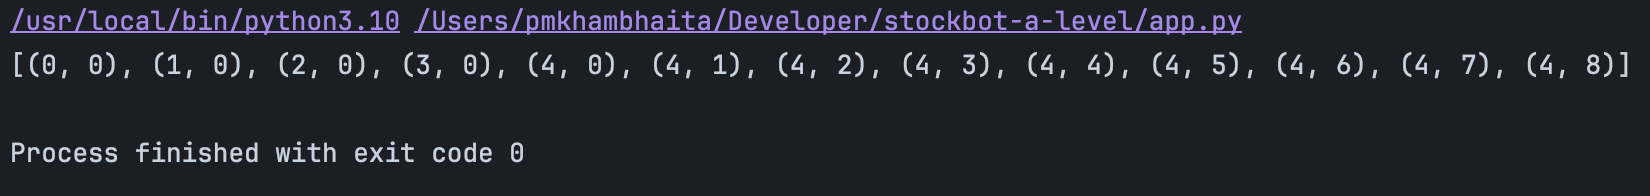
\includegraphics[width=0.8\textwidth]{Images/Screenshot 2025-03-30 at 11.18.52.png}
    \caption{The output of my algorithm with start at (0,0) and end at (4,8)}
\end{figure}

\subsubsection{Testing:}
\begin{table}[htbp]
\centering
\begin{tabularx}{\textwidth}{|l|X|p{3.5cm}|p{3.5cm}|c|}
\hline
\textbf{ID} & \textbf{Description} & \textbf{Expected} & \textbf{Actual} & \textbf{Pass?} \\
\hline
T1.1.1 & Input 0,0 and 9,9 & Direct path between both points & Direct path between points & X \\
\hline
T1.1.2 & Input 1,2 and 5,7 & Direct path between defined points only & Direct path between 1,2 and 5,7 & X \\
\hline
T1.1.3 & Input -1,-1 and 4,8 & Returns error & Error and break & \~{} \\
\hline
T1.1.4 & Input 0,1 and 10,10 & Return error & Error and break & \~{} \\
\hline

\end{tabularx}
\caption{Testing results for iteration 1}
\end{table}

\subsubsection{Tests justification}
These tests were for the main functionality of the program: the BFS must work because it is the heart of my program.
\subsubsection{Fixes}
T1.1.1 and T1.1.2 were successful, meaning the core functionality of the program is functional as expected. However, T1.1.3 and T1.1.4 were partially successful. While I did include the validation, I did not add a graceful error message, it was left to the basic python error-catching mechanisms. This will be fixed in the next iteration.

\subsubsection{Validation:}
\begin{itemize}
	\item Boundary check: I ensured that the new node \verb|(nx, ny)| is within the bounds of the graph
	\item Visited check: I checked that the new node \verb|(nx, ny)| has not been visited before.
\end{itemize}


\subsubsection{Review:}
\begin{itemize}
	\item Overall this iteration was quite successful. I managed to get a functional BFS algorithm working between 2 points, however I must be careful in not only validating but adding error messages for specific cases.
	\item Since this is still quite basic, I stuck to a simple procedural format rather than object-oriented principles. In the next iteration, I will be applying object-oriented principles as the program greatens in complexity.
\end{itemize}

\newpage

\subsubsection{Screenshots of tests/program}

\begin{figure}[htbp!]
    \centering
    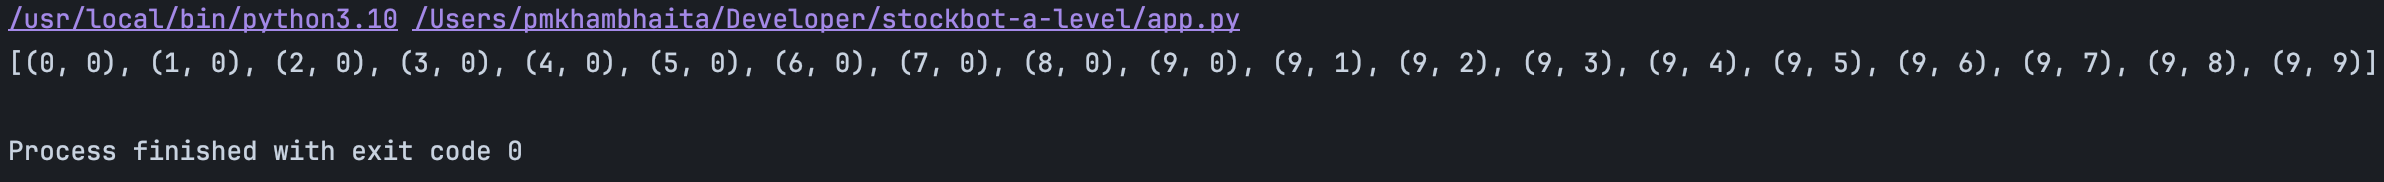
\includegraphics[width=1\linewidth]{Images/t1.1.png}
    \caption{T1.1.1 Output}
    \label{fig:enter-label}
\end{figure}

\begin{figure}[htbp!]
    \centering
    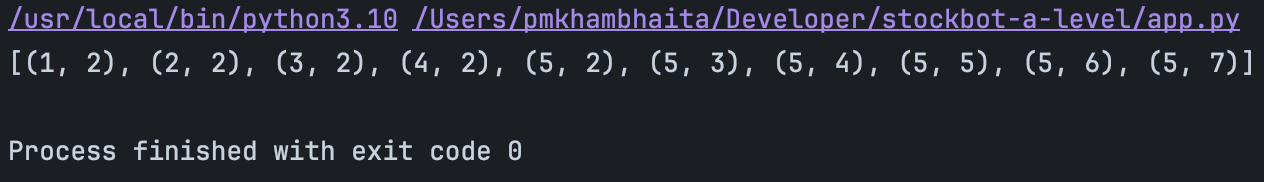
\includegraphics[width=1\linewidth]{Images/t1.2.png}
    \caption{T1.1.2 Output}
    \label{fig:enter-label}
\end{figure}

\begin{figure}[htbp!]
    \centering
    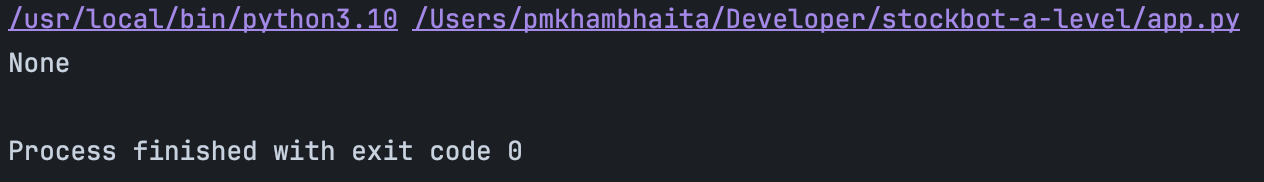
\includegraphics[width=1\linewidth]{Images/t1.3,1.4.png}
    \caption{T1.1.3 Output}
    \label{fig:enter-label}
\end{figure}

\begin{figure}[htbp!]
    \centering
    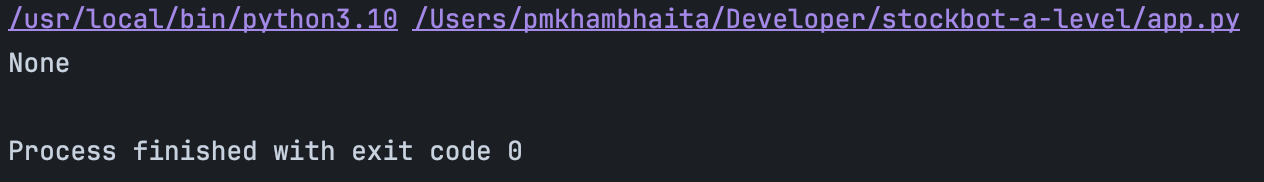
\includegraphics[width=1\linewidth]{Images/t1.3,1.4.png}
    \caption{T1.1.4 Output}
    \label{fig:enter-label}
\end{figure}


\newpage

\subsubsection{Iteration 2: Multi-point BFS and Visualisation}

\textbf{Code Changes:}
\begin{itemize}
    \item \textbf{GitHub Commits:} c90ad6a, 7f76931, 9f2e44b, c88ec49, 94fef19, bc69274, 8081015, 0499de6
    \item \textbf{Explanation:}
    Reviewing Iteration 1 highlighted that managing the BFS logic, user input, potential future state (like obstacles), and visualisation within a single procedural script was becoming unwieldy. Specifically, integrating the multi-point logic (OCSP-003)  and the terminal visualisation (OCSP-002)  required passing numerous parameters between functions, increasing the risk of errors and making code harder to read and debug. Therefore, transitioning to an Object-Oriented approach in Iteration 2 was justified to encapsulate related data and behaviour (Grid state, Pathfinding logic, Visualisation) into distinct classes, improving modularity, testability, and preparing the structure for future feature additions like the GUI."
\end{itemize}

\textbf{Code Quality:}
\begin{itemize}
    \item \textbf{Annotations added:} I annotated key methods and classes with simple comments as to what they did and any program-specific syntax like my labelling scheme for the visualisation.

    \item \textbf{Modular approach:} I have now implemented an object-oriented approach in my solution, splitting the grid and pathfinder logic into 2 separate classes, referenced by outer functions that process user input and output.
\end{itemize}

\newpage

\subsubsection{Code Implementation:}

\lstinputlisting[style=custompython]{Code/sa2.py}

\subsubsection{Prototype details:} 
The BFS algorithm is now working flawlessly, and I added some more debugging features like constant logging and output to the terminal using the \verb|logging| library within python. A timestamp and message is outputted when something of significance happens. The visualisation is also working excellently, and the user input is robust and easy to use. However, I do need to improve some parts of the logging, perhaps including the path the program will trace. As well as this, the path length is slightly inaccurate: it counts the start and end points, meaning it is 1 more than actual.

\begin{figure}[htbp]
    \centering
    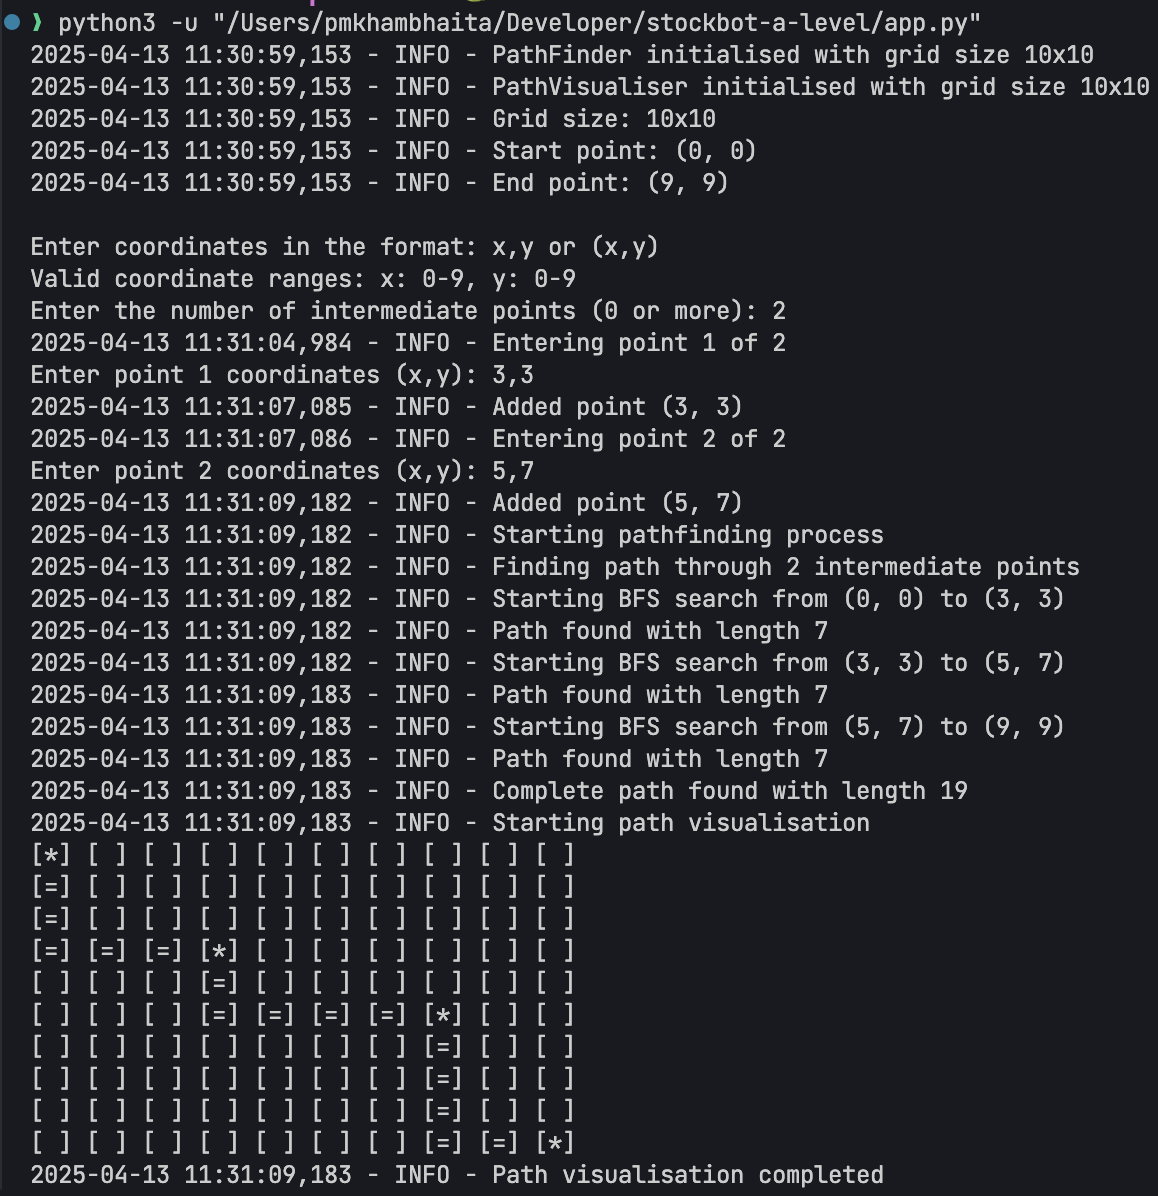
\includegraphics[width=0.6\textwidth]{Images/sa2test1.png}
    \caption{The output of my algorithm with points at (3,3) and end at (5,7)}
\end{figure}

\newpage

\subsubsection{Testing:}
\begin{table}[htbp]
\centering
\begin{tabularx}{\textwidth}{|l|X|p{3.5cm}|p{3.5cm}|c|}
\hline
\textbf{ID} & \textbf{Description} & \textbf{Expected} & \textbf{Actual} & \textbf{Pass?} \\
\hline
T1.2.1 & No intermediate points selected & Direct path between start and end & Direct path between start and end & X \\
\hline
T1.2.2 & Input 3,4 and 5,8 & Direct path between start and end stopping at defined points only & Direct path between start and end stopping at 3,4 and 5,8 & X \\
\hline
T1.2.3 & Input -1,-1 & Returns error & Returned graceful error and allowed retry & X \\
\hline
T1.2.4 & Input one valid and one non-valid point & Return error & Returned graceful error and allowed retry & X \\
\hline
T1.2.5 & Input 5 invalid points & Prevent entering from 1st points & Prevented addition of extra points until valid & X \\
\hline
T1.2.6 & Input valid points and verify it is the shortest path & Shortest path found & Shortest path found, path length incorrect & \~{} \\
\hline

\end{tabularx}
\caption{Testing results for iteration 1}
\end{table}

\subsubsection{Tests justification}
These tests were checking the validation measures I put in place for the SPA. These checked that all the validation was working, from boundary testing to existence validation. This was necessary to ensure the program is robust enough for the stakeholders and to cover all cases.


\subsubsection{Fixes}
Almost all tests were successful, and all previous errors have been resolved. However, the last test - T1.2.6 - was only a partial success - while the path was the shortest, the path length was out by +1. The issue was that the path length was being reported as the number of nodes in the path, but the actual path length should be the number of steps between nodes, which is one less than the number of nodes. Hence, I changed \verb|len(path)| to \verb|len(path) - 1|. This has been fixed in commit 121c011 and 1a7da80.

\newpage

\subsubsection{Screenshots of tests/program}

\begin{figure}[htbp!]
    \centering
    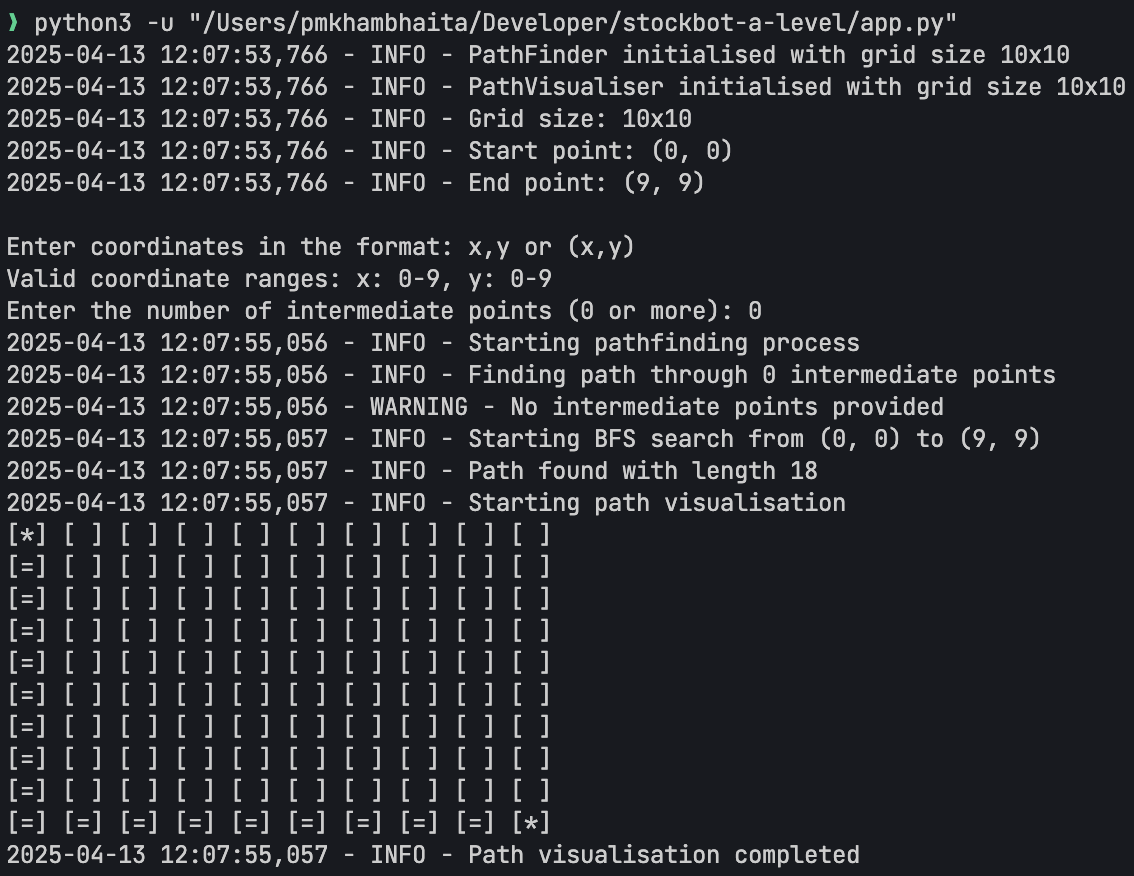
\includegraphics[width=0.5\linewidth]{Images/t1.2.1.png}
    \caption{T1.2.1 Output}
    \label{fig:enter-label}
\end{figure}

\begin{figure}[htbp!]
    \centering
    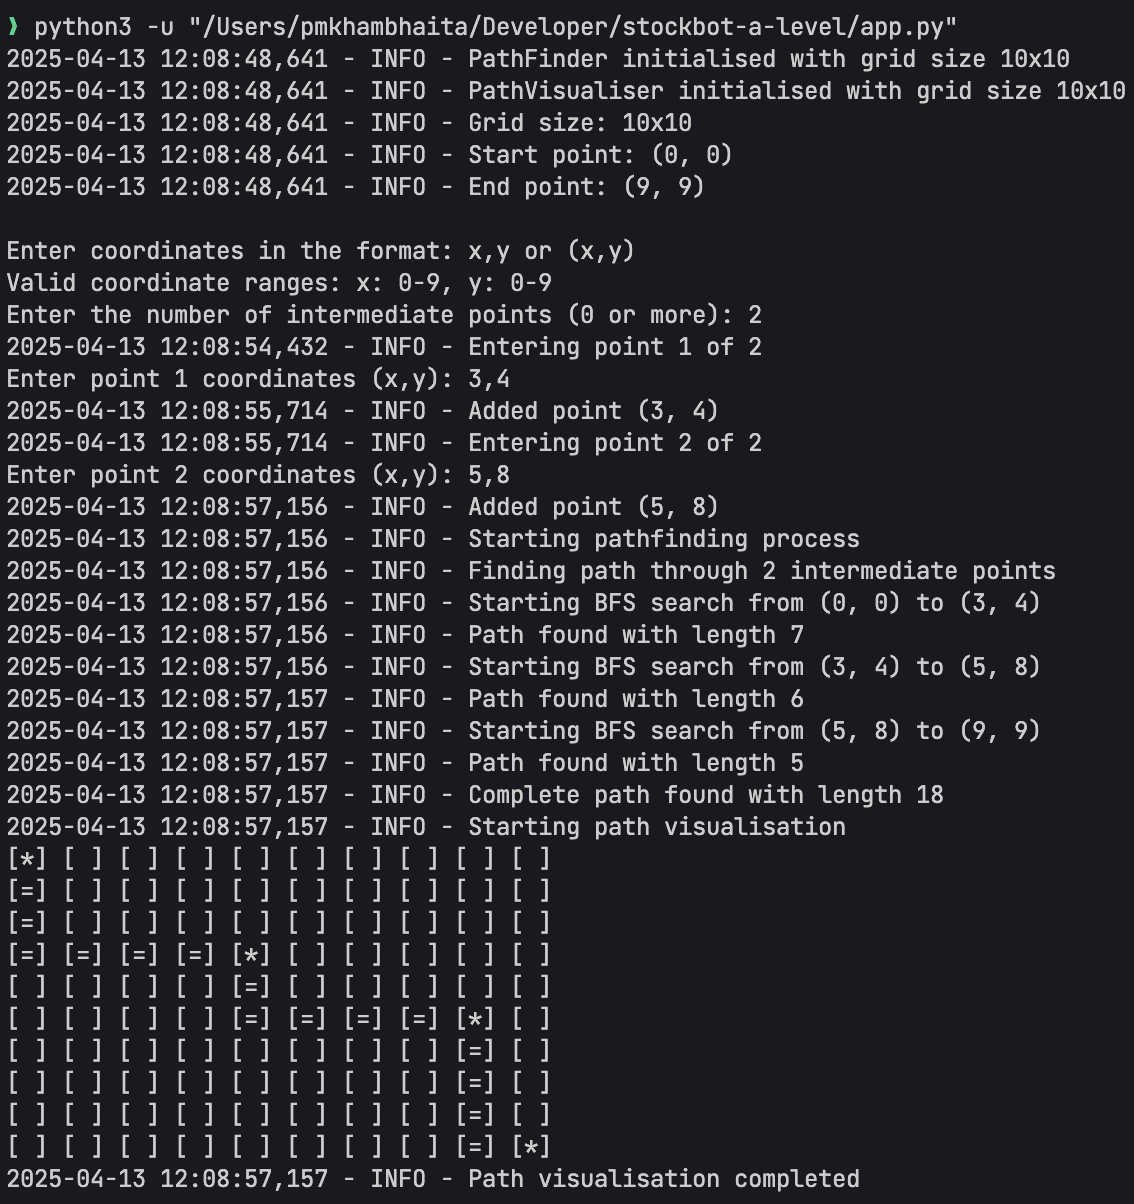
\includegraphics[width=0.5\linewidth]{Images/t1.2.2.png}
    \caption{T1.2.2 Output}
    \label{fig:enter-label}
\end{figure}

\begin{figure}[htbp!]
    \centering
    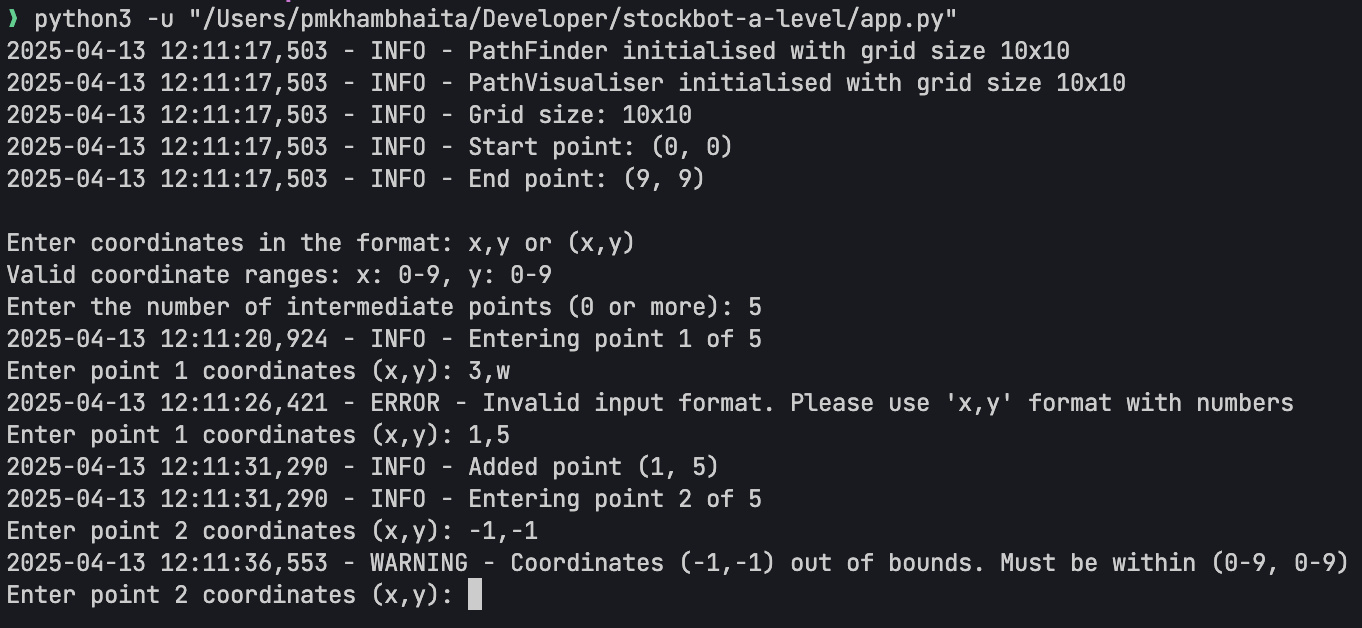
\includegraphics[width=0.5\linewidth]{Images/t1.2.x.png}
    \caption{T1.2.3/4/5 Output}
    \label{fig:enter-label}
\end{figure}

\begin{figure}[htbp!]
    \centering
    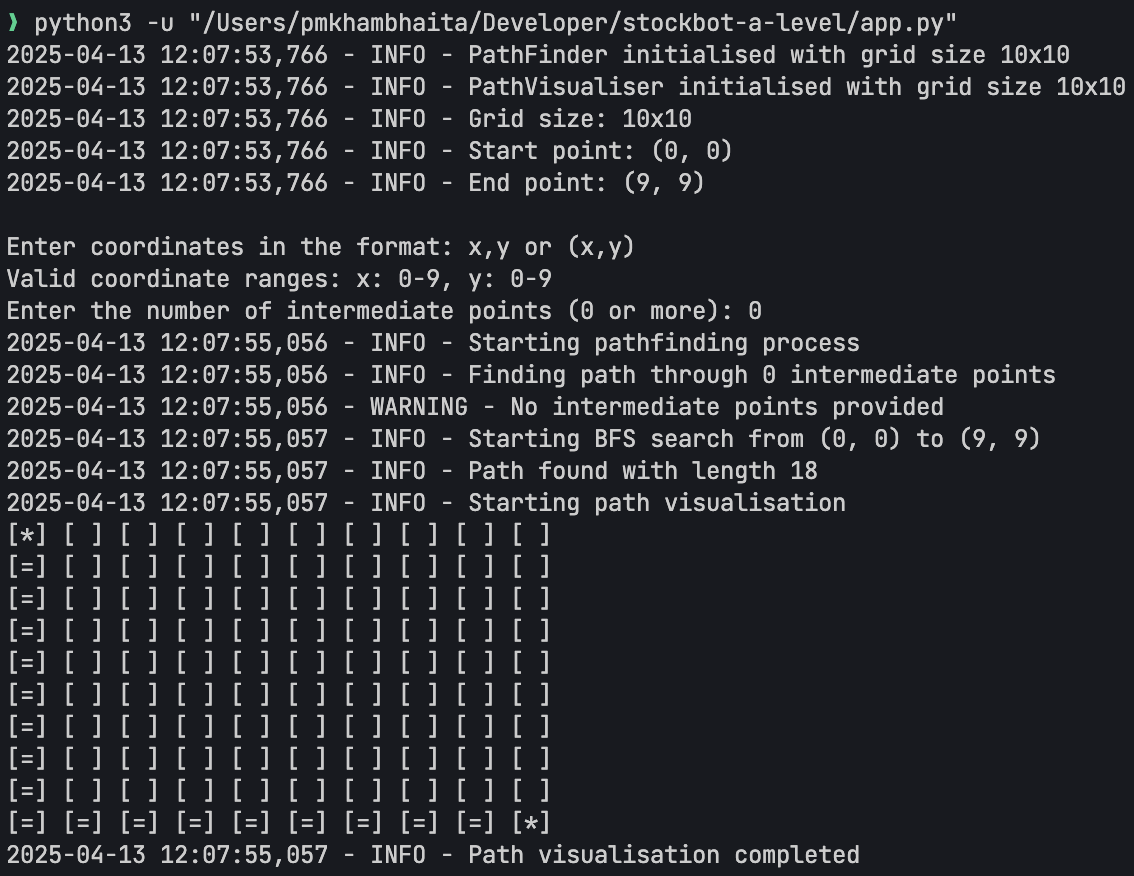
\includegraphics[width=0.5\linewidth]{Images/t1.2.1.png}
    \caption{T1.2.6 Output (fixed)}
    \label{fig:enter-label}
\end{figure}

\newpage

\subsubsection{Fixes}

The main issue I encountered was the path length being incorrect. After using my IDE's debugger and backtracking through my code, I found that the issue was the path-length counter; it was counting the nodes visited (the length of the path structure), not the path between them (nodes - 1). This was corrected by subtracting 1 from the length of the final path queue.

\subsubsection{Validation:}
\begin{itemize}
    \item \textbf{User input boundary \& range validation} - Confirms all user-provided points are within the grid boundaries and valid range of 0-9.
    \item \textbf{Type \& format validation} - Ensures coordinates are entered in the correct format (x,y) and contain valid numbers
    \item \textbf{Number of points validation} - Checks that the number of intermediate points entered is a non-negative integer
    \item \textbf{Path visualisation validation} - Confirms a path exists before attempting to visualise it
    \item \textbf{User point existence validation} - Handles the case where no intermediate points are provided
    \item \textbf{Exception handling} - Catches and logs any unexpected errors during program execution
\end{itemize}

\subsubsection{Review:}
 Overall this iteration was very successful. I have now completed what I set out to do in this sprint. There were some minor errors along the way, but they were fixed very quickly: they were mainly logic errors rather than syntax.

\clearpage
\subsection{Sprint Review and Retrospective}

\subsubsection{Accomplishments}
\begin{itemize}
    \item Completed OCSP-001 to OCSP-003
    \item  I have now successfully implemented the shortest path feature of my program, and is ready to use. Hence, the first stage of my design - getting a functional SPA running - is complete.
\end{itemize}

\subsubsection{Final testing}

This testing was recommended by my stakeholders; they each came up with 1 test in a certain area they would like me to perform. This testing was conducted using the data provided in Section x.x.x. In this case, since this program has only implemented the SPA, they will only be using the respective criteria:

\begin{itemize}
\item Grid is 15 x 15
\item Points using random num gen between 0 and 14 (x2): (2,5), (8,9), (10,2) 

\end{itemize}

\begin{table}[htbp]
\centering
\begin{tabularx}{\textwidth}{|l|X|p{3.5cm}|p{3.5cm}|c|}
\hline
\textbf{ID} & \textbf{Description} & \textbf{Expected} & \textbf{Actual} & \textbf{Pass?} \\
\hline
T1.F.1 & Path found using input points & Path between start and end including user-defined points& Direct path between start and end stopping at (2,5), (8,9) and (10,2)  & X \\
\hline
T1.F.2 & Input invalid points (letters, numbers and symbols) & Warns user that points are invalid & Prevents user from entering the points and displays a descriptive message & X \\
\hline
T1.F.3 & Input no points &  Direct path between start and end & Direct path between start and end & X \\
\hline
\end{tabularx}
\end{table}

\subsubsection{Testing Summary}
\begin{table}[htbp]
\centering
\begin{tabular}{|l|c|}
\hline
\textbf{Metric} & \textbf{Count} \\
\hline
Total tests conducted & 13 \\
\hline
Tests passed & 11 \\
\hline
Tests failed & 2 \\
\hline
Fixed issues & 3 \\
\hline
\end{tabular}
\caption{Sprint 1 testing summary}
\end{table}

\subsubsection{Validation}
    \begin{itemize}
    \item \textbf{Grid Boundary Validation for Start/End Points} - Checks if coordinates are within grid dimensions
    \item \textbf{User Input Format Validation} - Validates coordinate input format (x,y)
    \item \textbf{User Input Range Validation} - Confirms coordinates are within valid grid dimensions
    \item \textbf{Number of Points Validation} - Ensures number of intermediate points is non-negative
    \item \textbf{Path Existence Validation} - Verifies if a valid path exists between points
    \item \textbf{Intermediate Point Boundary Validation} - Ensures user-provided points are within grid boundaries
    \item \textbf{Path Visualisation Validation} - Checks if a path exists before attempting visualisation
\end{itemize}

\subsubsection{Robustness}
\begin{itemize}
    \item \textbf{Exception Handling} -- Uses try-except blocks to catch and log unexpected errors
    \item \textbf{Logging Implementation} -- Comprehensive logging of program flow and errors
    \item \textbf{Default Parameter Values} -- Uses None as default for optional parameters
    \item \textbf{Queue Management in BFS} -- Properly manages the queue in breadth-first search
    \item \textbf{Path Segment Validation} -- Validates each segment of the multi-point path
    \item \textbf{Keyboard Interrupt Handling} -- Catches user interruptions during input collection
    \item \textbf{Consistent Return Values} -- Functions return None for failure cases
    \item \textbf{Empty Points List Handling} -- Gracefully handles cases with no intermediate points
\end{itemize}

\subsubsection{Stakeholder Review}

I am currently happy with progress made. The BFS algorithm seems very promising and does show potential for speeding up operations. (Minash Khambhaita, Primary Stakeholder)

\subsubsection{Link}

With the completion of this sprint, I have now created one complete feature that was requested by the stakeholders: the shortest path algorithm. From the design section, I have successfully implemented BFS to shorten the time taken to collect items, which means I have met one of the requirements from the stakeholders. This is because BFS has significantly reduced the time taken to find an optimal path, the main purpose of my solution. \newline The next sprint will focus on creating the GUI and adding more usability features to make the program easy to use: currently it is still terminal-based. (see the design breakdown)


\clearpage

% Berners-Lee

\section{Sprint Berners-Lee}

This is Sprint Berners-Lee, the second iteration of my program. This iteration focuses on developing the Graphical User Interface (GUI) using Tkinter, replacing the previous terminal-based interaction. The goal is to provide a more user-friendly way to input points and visualise the shortest path generated by the existing SPA (Shortest Path Algorithm) logic. This sprint intends to create a functional GUI only, with a later sprint focussed on adding more usability features and making the GUI look more like what the stakeholders were expecting.

\subsection{Tasks}

\begin{table}[htbp]
	\centering
	\begin{tabularx}{\textwidth}{|l|X|}
		\hline
		\textbf{Task ID} & \textbf{Task Description} \\
		\hline
		OCSP-004 & Project Restructure: Reorganise code by separating GUI logic (\verb|gui.py|) from the core pathfinding logic (\verb|spa.py|) for better modularity. \\
		\hline
		OCSP-005 & GUI Scaffolding: Create the basic Tkinter window structure, input fields (point entry), output area (text box), and control buttons (\verb|Add Point|, \verb|Find Path|, \verb|Clear|). Implement layout using the \verb|grid| manager. \\
		\hline
		OCSP-006 & GUI-SPA Integration: Connect GUI elements to the backend \verb|spa.py| classes (\verb|Grid|, \verb|PathFinder|, \verb|PathVisualiser|). Implement functionality for adding points, triggering pathfinding, and clearing inputs via button clicks. \\
		\hline
		OCSP-007 & Visualisation Output Redirection: Capture the standard output of the \verb|visualise_path| method (which previously printed to terminal) and display it within the GUI's text output area. \\
		\hline
		OCSP-008 & Validation Integration \& Error Handling: Revamp the validation by creating a single function to handle robust input validation, preventing invalid coordinates (out of bounds, start/end points, incorrect format) and providing clear error messages directly in the GUI output area. Remove redundant terminal-based input functions. \\
		\hline
		OCSP-009 & Logging Enhancement: Implement logging to a dedicated file (\verb|stockbot_log.txt|) alongside terminal logging for persistent debugging information. \\
		\hline
		OCSP-010 & GUI Refinements: Improve clarity of error messages, ensure GUI starts cleanly without residual terminal interactions, and add a textual representation of the path sequence to the output. \\
		\hline
	\end{tabularx}
\end{table}

\subsection{Purpose}

This sprint aims to significantly enhance usability by transitioning from a command-line interface to a graphical one. This addresses the stakeholders' need for a more intuitive user experience, allowing users to easily input intermediate points and view the calculated shortest path, including a visual grid representation, directly within a dedicated application window.

\clearpage
\subsection{Sprint Planning Details}

\subsubsection{Technical Approach}

This GUI implementation uses Python's built-in Tkinter library. This choice was justified by its inclusion in the standard library (avoiding external dependencies) as well as the fact it is both powerful and sufficient for the project's UI complexity.

\begin{enumerate}
	\item \textbf{Restructure:} Separate existing SPA logic (\verb|app.py| renamed to \verb|spa.py|) from new GUI code (\verb|gui.py|). (OCSP-004)
	\item \textbf{Create basic GUI layout:} Use Tkinter's \verb|grid| geometry manager to begin placing basic components on the page. (OCSP-005)
	\item \textbf{Event Handling:} Implement methods (\verb|add_point|, \verb|find_path|, \verb|clear_all|) triggered by button clicks. (OCSP-006)
	\item \textbf{Input Handling:} Retrieve and parse user input from the \verb|ttk.Entry| widget. (OCSP-006)
	\item \textbf{Output Redirection:} Use \verb|io.StringIO| and \verb|sys.stdout| redirection to capture the printed output of \verb|path_visualiser.visualise_path| and insert it into the \verb|tk.Text| widget. (OCSP-007)
	\item \textbf{Validation:} Refine the validation by creating a single dedicated validation function (\verb|validate_point| in \verb|spa.py|) checking boundaries and start/end point exclusion; this will be called from the GUI's \verb|add_point| method. Display validation errors directly in the GUI's output text area. Remove old terminal input functions (\verb|get_valid_coordinate|, \verb|get_points|) from \verb|spa.py|. (OCSP-008)
	\item \textbf{Logging:} Configure the \verb|logging| module in \verb|spa.py| to add a \verb|FileHandler|, directing logs to \verb|stockbot_log.txt| in addition to the console. (OCSP-009)
	\item \textbf{Refinements:} Improve error message wording for clarity. Add textual path sequence output (\verb|(0,0) -> (1,0) -> ...|) to the GUI. Ensure the main execution block in \verb|spa.py| (which previously ran the terminal version) is removed to prevent interference. (OCSP-010)
\end{enumerate}

\subsubsection{Architecture \& Structural Considerations}

The architecture now consists of two main Python files:
\begin{itemize}
	\item \verb|spa.py|: Contains the backend logic classes (\verb|Grid|, \verb|PathFinder|, \verb|PathVisualiser|) and helper functions (\verb|validate_point|). It also handles logging configuration. The classes remain largely unchanged from Sprint Ada, ensuring the core pathfinding algorithm is stable.
	\item \verb|gui.py|: Introduces the \verb|PathfinderGUI| class, responsible for creating and managing all Tkinter widgets. It allows user interaction, calling methods from \verb|spa.py| for validation and pathfinding, and displaying results.
\end{itemize}

\newpage

\subsection{Development Summary}


\subsubsection{Iteration 1}
\begin{itemize}
	\item \textbf{Progress made:}
	\begin{itemize}
		\item OCSP-004: Restructured project, separating \verb|gui.py| and \verb|spa.py|.
		\item OCSP-005: Set up basic Tkinter window (\verb|PathfinderGUI| class), configured \verb|grid| layout manager, added input entry, output text area, and control buttons.
		\item OCSP-006: Initialised backend components (\verb|Grid|, \verb|PathFinder|, etc.) within the GUI class method \verb|__init__|. Implemented basic \verb|add_point|, \verb|find_path|, \verb|clear_all| methods and linked them to buttons. Connected \verb|add_point| to basic boundary check and \verb|find_path| to call the backend pathfinding.
		\item OCSP-007: Implemented output redirection using \verb|io.StringIO| to display the visualiser's grid output in the GUI text area.
	\end{itemize}
	\item \textbf{Blockers identified:}
	\begin{itemize}
		\item The terminal interface defined in \verb|spa.py|'s main execution block was still running alongside the GUI.
		\item Basic validation allowed adding start/end points (0,0 or 9,9) as intermediate points.
		\item Error messages were logged to the terminal via \verb|spa.logger| but not displayed within the GUI itself.
	\end{itemize}
	\item \textbf{Plan for next iteration:}
	\begin{itemize}
		\item Remove residual terminal code execution from \verb|spa.py|.
		\item Implement stricter validation to prevent adding start/end points.
		\item Integrate error/warning messages directly into the GUI output area.
	\end{itemize}
\end{itemize}

\subsubsection{Iteration 2}
\begin{itemize}
	\item \textbf{Progress made:}
	\begin{itemize}
		\item OCSP-008: Created \verb|validate_point| function in \verb|spa.py| to check boundaries AND prevent adding start/end points. Modified GUI \verb|add_point| to use this new function. Removed old terminal input functions (\verb|get_valid_coordinate|, \verb|get_points|) and main execution block from \verb|spa.py|
		\item OCSP-009: Configured logging in \verb|spa.py| to output to \verb|stockbot_log.txt|.
		\item OCSP-008, OCSP-010: Modified GUI methods (\verb|add_point|, \verb|find_path|) to display error messages (invalid format, no points added, validation failures) directly in the \verb|output_text| widget.
	\end{itemize}
	\item \textbf{Blockers identified:}
	\begin{itemize}
		\item Error message wording could be more user-friendly/specific (e.g., format error message).
		\item The GUI shows the visual grid path but doesn't list the sequence of coordinates followed.
	\end{itemize}
	\item \textbf{Plan for next iteration:}
	\begin{itemize}
		\item Refine error message text for better clarity.
		\item Add the sequence of path coordinates to the output.
	\end{itemize}
\end{itemize}

\subsubsection{Iteration 3}
\begin{itemize}
	\item \textbf{Progress made:}
	\begin{itemize}
		\item OCSP-010: Improved error messages in \verb|gui.py| for invalid format, start/end point conflict, and out-of-bounds errors to be more intuitive. Made the "no points added" error more specific.
		\item OCSP-010: Added functionality to display the textual sequence of the path coordinates (e.g., \verb|(0,0) -> (1,0) -> ...|) in the GUI output area after the grid visualisation.
	\end{itemize}
\end{itemize}

\clearpage
\subsection{Sprint Berners-Lee Implementation}

\subsubsection{Iteration 1: Getting GUI Working}

\textbf{Code Changes:}
\begin{itemize}
	\item \textbf{GitHub Commits:} \verb|dc29116|, \verb|51caad0|, \verb|2cc86ce|, \verb|93cddaa|, \verb|256e1a2| (partially - validation function creation), \verb|be7179a| (partially - removing terminal execution)
	\item \textbf{Explanation:}
	\begin{itemize}
		\item Project structure was refactored by creating \verb|gui.py| for Tkinter code and renaming \verb|app.py| to \verb|spa.py| to hold the backend logic. This separation improves organisation.
		\item The basic \verb|PathfinderGUI| class was created using Tkinter. The window layout was defined using the \verb|grid| manager for better control over widget placement compared to \verb|pack|. Key widgets (Entry for points, Text for output, Buttons for Add/Find/Clear) were added and placed.
		\item Backend components (\verb|Grid|, \verb|PathFinder|, \verb|PathVisualiser| from \verb|spa.py|) were instantiated within the GUI \verb|__init__| method.
		\item Button commands were linked to placeholder or initial implementation methods (\verb|add_point|, \verb|find_path|, \verb|clear_all|).
		\item The standard output of the \verb|path_visualiser.visualise_path| method was captured using \verb|io.StringIO| via the redirection of \verb|sys.stdout|, allowing the text-based grid visualisation to be displayed within the GUI's text widget (\verb|self.output_text|).
		\item The terminal execution block in \verb|spa.py| was removed to prevent the command-line interface from running simultaneously with the GUI.
	\end{itemize}
\end{itemize}

\textbf{Code Quality:}
\begin{itemize}
	\item \textbf{Annotations added:} Basic comments added outlining the purpose of GUI elements and methods. Need to ensure comments aid future maintenance as per previous feedback.
	\item \textbf{Variable/Structure naming:} Followed conventions (e.g., \verb|point_entry|, \verb|output_text|, \verb|path_finder|). Names clearly indicate the purpose of GUI elements and backend component instances.
	\item \textbf{Modular approach:} Significant improvement through separation of GUI (\verb|gui.py|) and backend (\verb|spa.py|) logic. The \verb|PathfinderGUI| class encapsulates all GUI-related state and behaviour.
\end{itemize}

\newpage % Placeholder Start: Iteration 1 Code Snippets

\subsubsection*{Prototype: Iteration}
\subsubsection{gui.py}
\lstinputlisting[style=custompython]{Code/guisb1.py}

\subsubsection{spa.py}
\lstinputlisting[style=custompython]{Code/spasb1.py}


\subsubsection{Prototype details:}
At the end of this iteration, a basic GUI window appears with input fields and buttons. Users can add points (with basic boundary checks), trigger pathfinding, and see the grid visualisation printed. Clearing points and output is functional. However, validation is incomplete (allows start/end points), and error messages are primarily logged rather than shown in the GUI. This will be fixed in future iterations dedicated to patching error handling and other small issues.

\subsubsection{Testing:}

\begin{table}[htbp]
	\centering
	\begin{tabularx}{\textwidth}{|l|X|p{5.5cm}|p{2.8cm}|c|}
		\hline
		\textbf{ID} & \textbf{Description} & \textbf{Expected} & \textbf{Actual} & \textbf{Pass?} \\
		\hline
		T2.1.1 & Run script & Only GUI appears & Met & X \\
		\hline
		T2.1.2 & Launch GUI & Window appears with input field, text area, Add/Find/Clear buttons & Met & X \\
		\hline
		T2.1.3 & Add valid point (e.g., 3,4) & Point added, confirmation in output text & Met & X \\
		\hline
		T2.1.4 & Add multiple valid points & Points added sequentially & Met & X \\
		\hline
		T2.1.5 & Click \verb|Find Path| with points & Grid visualisation appears in output text & Met & X \\
		\hline
		T2.1.6 & Click \verb|Clear| & Points list cleared, output area cleared & Met & X \\
		\hline
		T2.1.7 & Add start point (0,0) & Should be disallowed eventually, but currently adds point & Point added & * \\
		\hline
		T2.1.8 & Add out-of-bounds point (-1,5) & Point rejected, error ideally in GUI & Point rejected, logged to console &\~{} \\
		\hline
	\end{tabularx}
	\caption{Testing results for iteration 2}
\end{table}


\subsubsection{Fixes}
No specific fixes applied in this iteration, but issues requiring fixes were identified: preventing start/end point addition, displaying errors in the GUI, and removing the remaining redundant terminal execution functions.

\subsubsection{Validation}

Validation is still constant as of this iteration, but in the coming iterations, it will be unified under a single function.

\newpage % Placeholder Start: Iteration 1 Screenshots

\subsubsection*{Iteration 1 Screenshots}

\begin{figure}[htbp!]
	\centering
	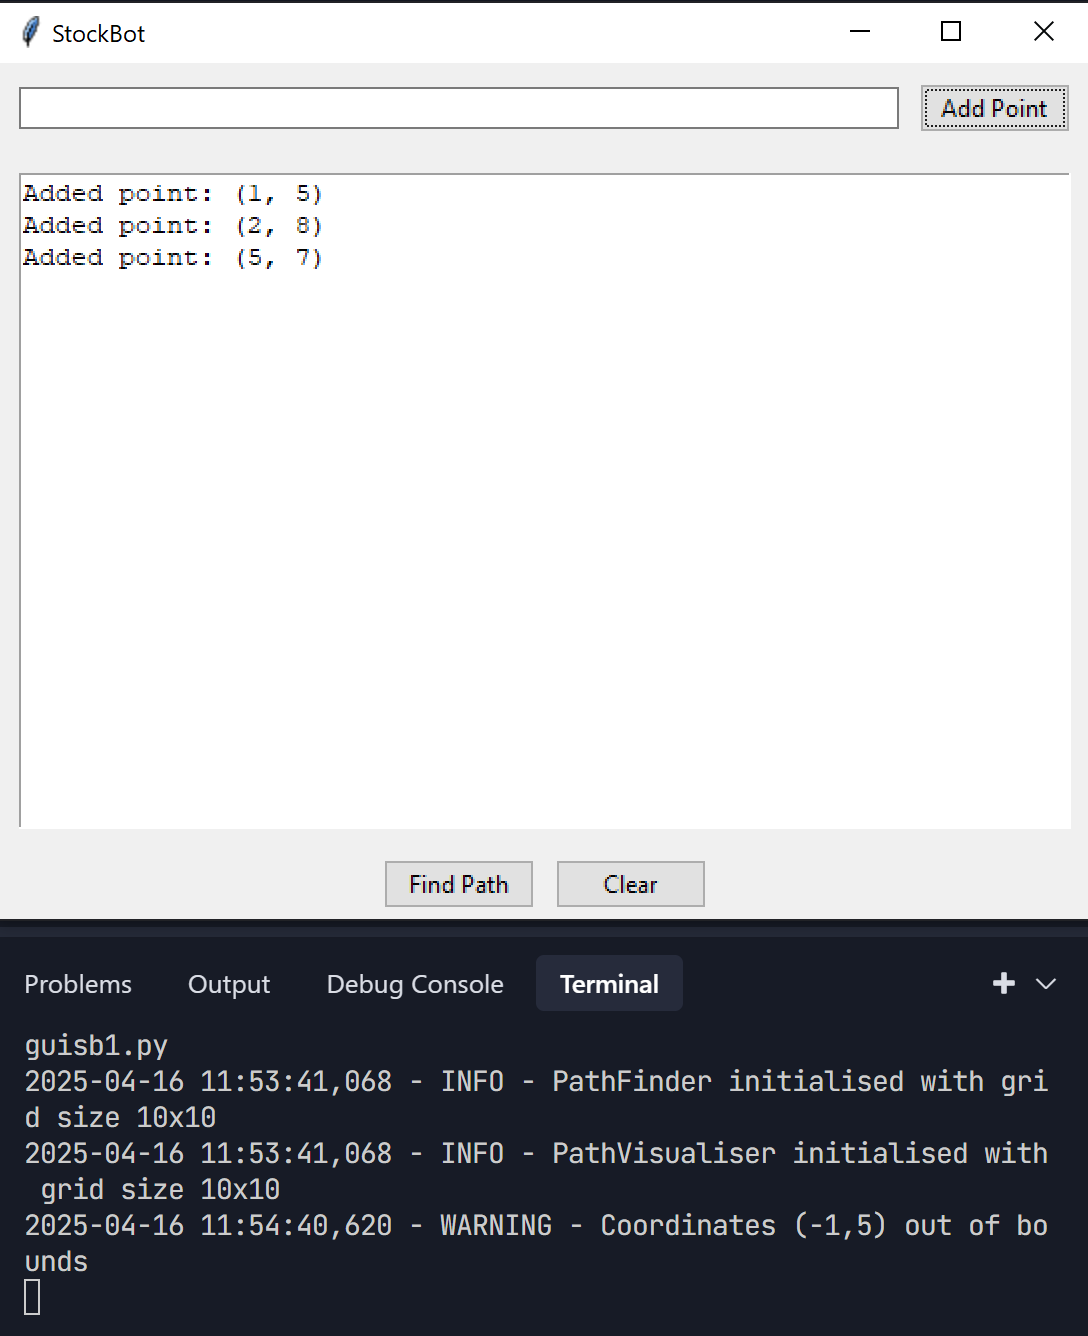
\includegraphics[width=0.35\linewidth]{Images/sprintbtest1.png}
	\caption{T2.1.1-T2.1.4, T2.1.8 Output}
\end{figure}

\begin{figure}[htbp!]
	\centering
	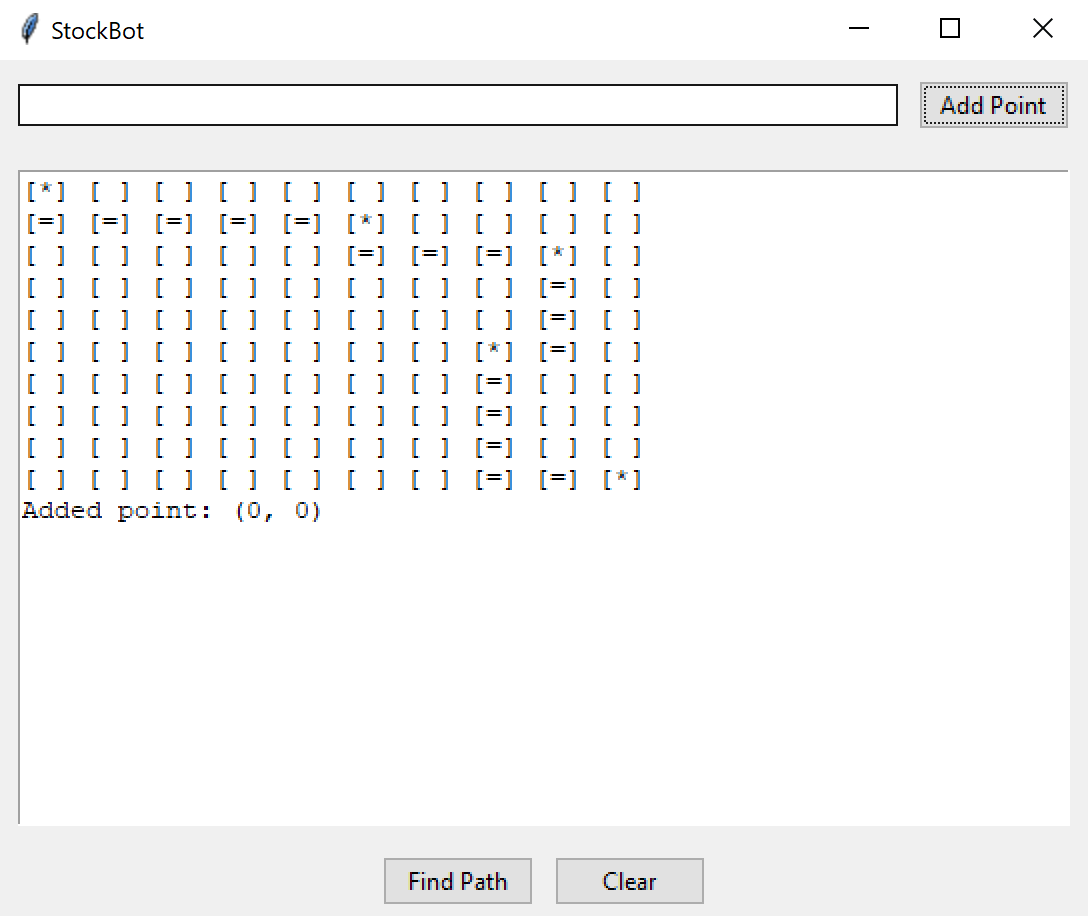
\includegraphics[width=0.4\linewidth]{Images/sprintbtest2.png}
	\caption{T2.1.5/2.1.7 Output}
\end{figure}

\begin{figure}[htbp!]
	\centering
	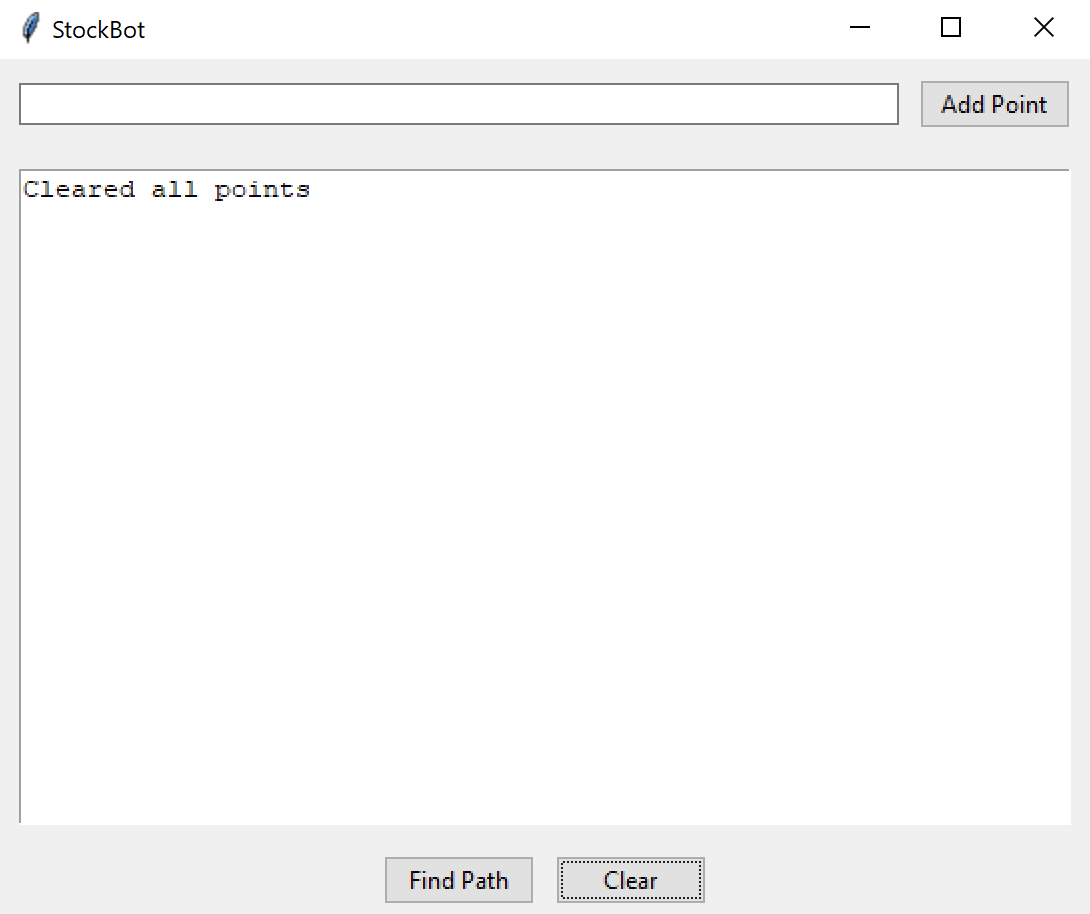
\includegraphics[width=0.4\linewidth]{Images/sprintbtest3.png}
	\caption{T2.1.6 Output}
\end{figure}

\newpage


\subsubsection{Iteration 2: Refining Logic and Validation}

\textbf{Code Changes:}
\begin{itemize}
	\item \textbf{GitHub Commits:} \verb|256e1a2| (most), \verb|be7179a| (most), \verb|babafb7|, \verb|9c248be| (partially - initial error integration)
	\item \textbf{Explanation:}
	\begin{itemize}
		\item Centralised validation logic by creating the \verb|validate_point| function in \verb|spa.py|. This function checks both grid boundaries and ensures the point is not the fixed start (0,0) or end (grid max) node. This addressed the blocker identified in Iteration 1.
		\item The \verb|add_point| method in \verb|gui.py| was refactored to call \verb|spa.validate_point|. Logic was added to display specific error messages within the GUI's \verb|output_text| widget if validation fails (e.g., "Cannot add point... Must not be start/end point...") or if the input format is incorrect.
		\item The now-redundant terminal input functions (\verb|get_valid_coordinate|, \verb|get_points|) were removed from \verb|spa.py|.
		\item Logging was enhanced in \verb|spa.py| by adding a \verb|FileHandler| to output logs to \verb|stockbot_log.txt|, providing a persistent record for debugging alongside the console output.
		\item Error reporting for cases like "No points added" or "No valid path found" within the \verb|find_path| method was modified to output directly to the GUI text area.
	\end{itemize}
\end{itemize}

\textbf{Code Quality:}
\begin{itemize}
	\item \textbf{Annotations added:} Docstring added for \verb|validate_point|. Comments explaining GUI error message integration.
	\item \textbf{Modular approach:} Strengthened by centralising point validation in \verb|spa.py| and removing unused terminal functions. GUI handles user interaction and display, backend handles validation and pathfinding.
	\item \textbf{Robustness:} Significantly improved by adding validation against start/end points and displaying user-facing error messages directly in the GUI for invalid input or missing points, addressing issues from Iteration 1. Added file logging for better diagnostics.
\end{itemize}

\newpage % Placeholder Start: Iteration 2 Code Snippets


\subsubsection*{Prototype: Iteration 2}
\subsubsection{gui.py}
\lstinputlisting[style=custompython]{Code/guisb2.py}

\newpage

\subsubsection{spa.py}
\lstinputlisting[style=custompython]{Code/spasb2.py}

\newpage % Placeholder End: Iteration 2 Code Snippets

\subsubsection{Prototype details:}
The GUI now correctly prevents adding start/end points and points outside boundaries, providing error feedback within the application window. Errors for invalid format or attempting to find a path with no points are also shown in the GUI. Backend logging is now saved to \verb|stockbot_log.txt| - this is to aid debugging in the future now my program is growing in complexity.

\subsubsection{Testing:}
\begin{table}[htbp]
	\centering
	\begin{tabularx}{\textwidth}{|l|X|p{4.5cm}|p{1.5cm}|c|}
		\hline
		\textbf{ID} & \textbf{Description} & \textbf{Expected} & \textbf{Actual} & \textbf{Pass?} \\
		\hline
		T2.2.1 & Add start point (0,0) & Rejected, error message in GUI & Met & X \\
		\hline
		T2.2.2 & Add end point (9,9) & Rejected, error message in GUI & Met & X \\
		\hline
		T2.2.3 & Add out-of-bounds point (-1,5) & Rejected, error message in GUI & Met & X \\
		\hline
		T2.2.4 & Enter invalid format ('abc') & Rejected, error message in GUI & Met & X \\
		\hline
		T2.2.5 & Click \verb|Find Path| with no points & Error message in GUI & Met & X \\
		\hline
		T2.2.6 & Perform valid path operation & Path visualisation in GUI, log entries in \verb|stockbot_log.txt| & Met & X \\
		\hline
	\end{tabularx}
	\caption{Testing results for iteration 2.2}
\end{table}

\subsubsection{Fixes}
Addressed issues from Iteration 1:
\begin{itemize}
	\item Prevented adding start/end points via \verb|validate_point| and GUI logic.
	\item Integrated error messages directly into the GUI output area.
	\item Removed conflicting terminal code from \verb|spa.py|.
\end{itemize}

\subsubsection{Validation}

\begin{itemize}
	\item Centralised Validation (\verb|validate_point|): Implemented checks for boundaries AND exclusion of start/end points (0,0 and 9,9) in \verb|spa.py|.
	\item GUI Integration: \verb|add_point| now calls \verb|validate_point| and displays returned error messages in the GUI.
	\item Input Existence Check: \verb|find_path| checks if \verb|self.points| list is empty before proceeding.
	\item Format Validation (try-except): Remains from Iteration 1, now with GUI error display.
\end{itemize}

These validation methods build upon the first sprint, but now focussing more on input validation, as the input method has changed from a terminal-based environment to a GUI.

\newpage

\subsubsection*{Iteration 2 Screenshots}
\begin{figure}[htbp!]
	\centering
	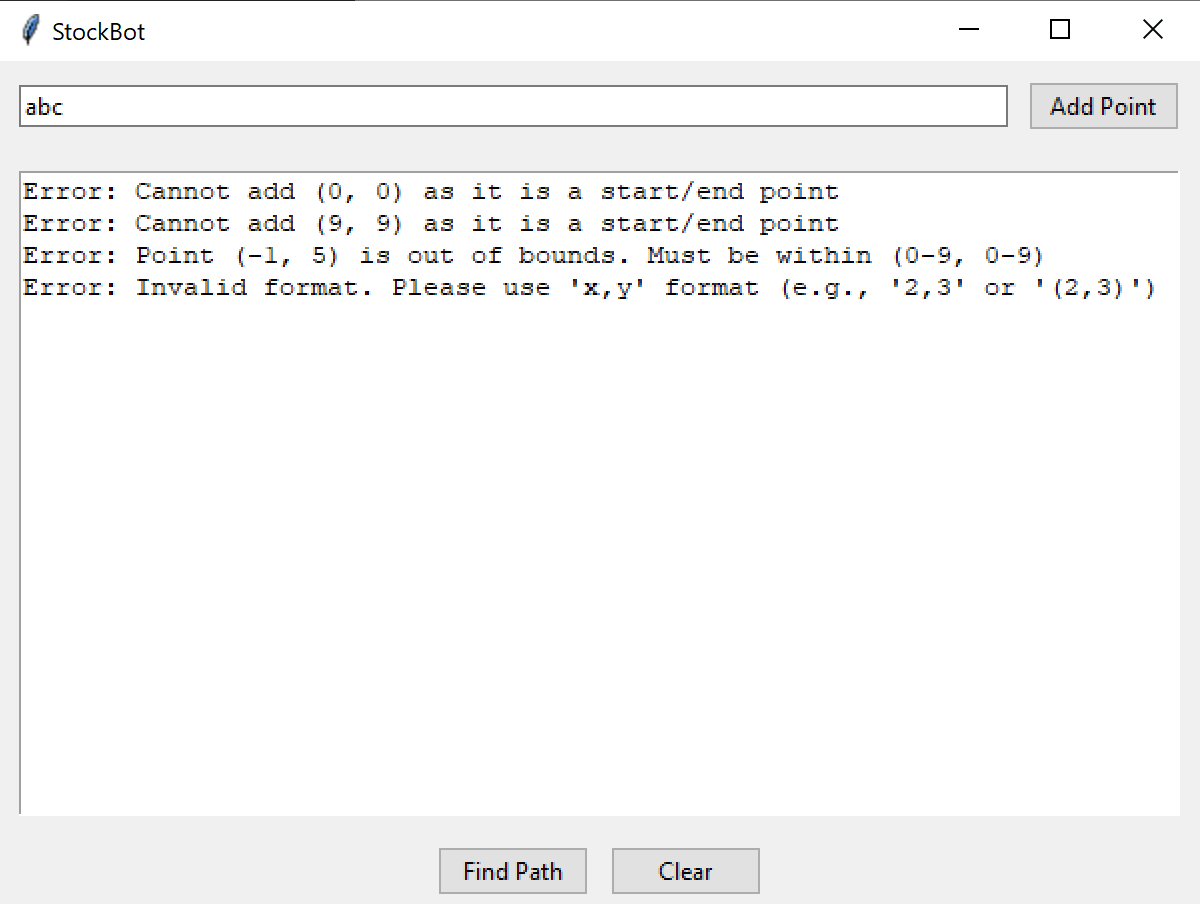
\includegraphics[width=0.45\linewidth]{Images/t2.2.x.png}
	\caption{T2.2.1-T2.2.4 Output}
	\label{fig:enter-label}
\end{figure}

\begin{figure}[htbp!]
	\centering
	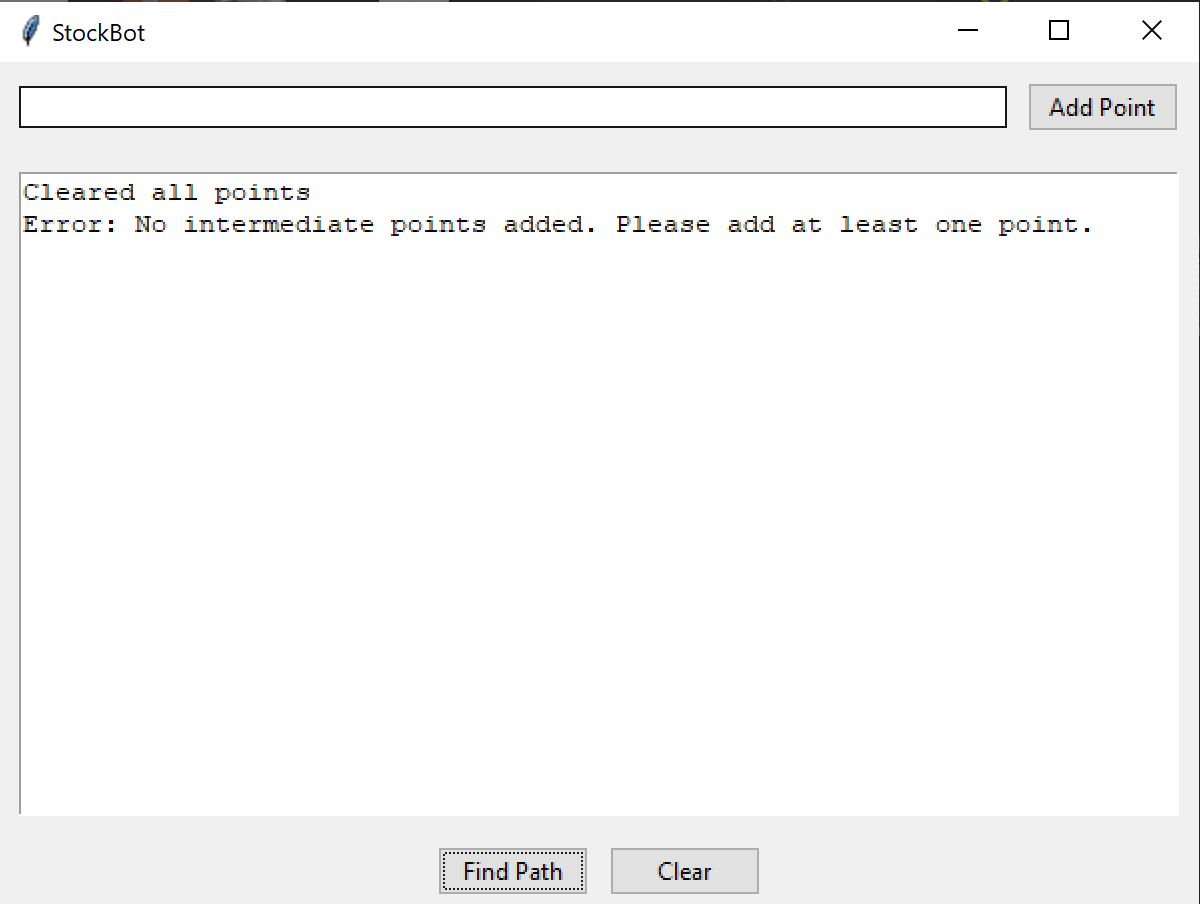
\includegraphics[width=0.45\linewidth]{Images/t2.2.x1.png}
	\caption{T2.2.5 Output}
	\label{fig:enter-label}
\end{figure}

\begin{figure}[htbp!]
	\centering
	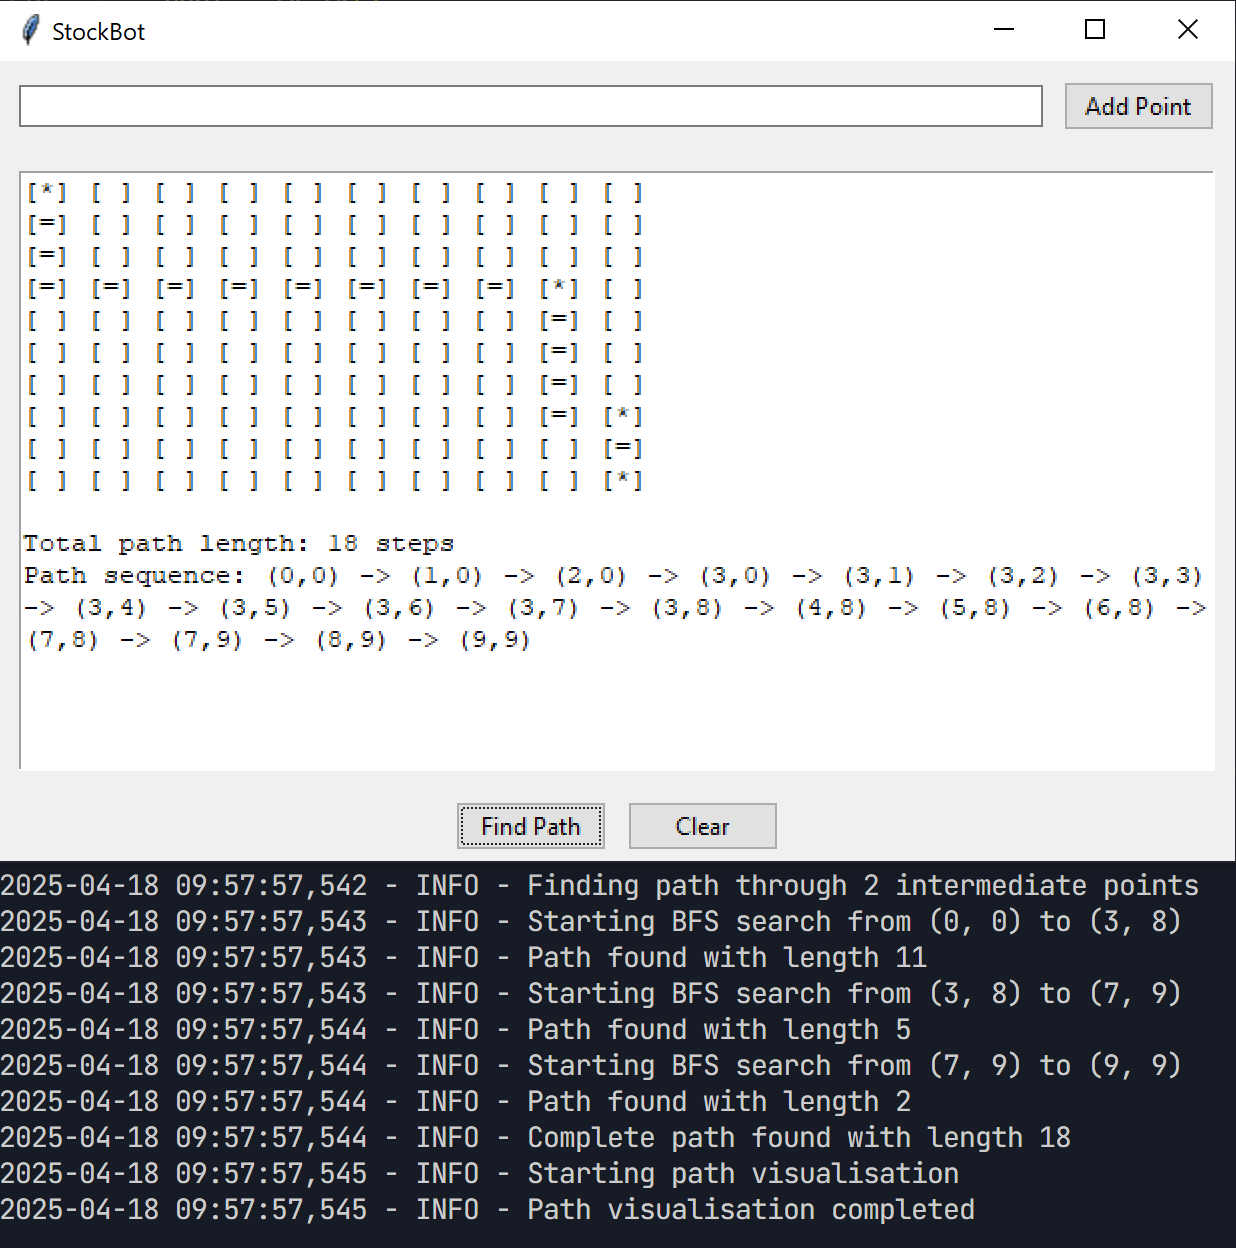
\includegraphics[width=0.45\linewidth]{Images/t2.2.6.png}
	\caption{T2.2.6 Output}
	\label{fig:enter-label}
\end{figure}

\newpage % Placeholder End: Iteration 2 Screenshots

\clearpage
\subsection{Sprint Review and Retrospective}

\subsubsection{Accomplishments}
\begin{itemize}
	\item Completed OCSP-004: Project restructured into \verb|spa.py| (backend) and \verb|gui.py| (frontend).
	\item Completed OCSP-005: GUI with Tkinter widgets and \verb|grid| manager implemented.
	\item Completed OCSP-006: GUI controls successfully linked to backend pathfinding logic.
	\item Completed OCSP-007: Path visualisation output displayed correctly within the GUI text area.
	\item Completed OCSP-008: Robust validation for point input (format, bounds, start/end exclusion) integrated into the GUI with error messages. Redundant terminal functions removed.
	\item Completed OCSP-009: Logging to \verb|stockbot_log.txt| implemented for persistent diagnostics.
	\item Completed OCSP-010: GUI error messages refined for clarity, path sequence output added.
	\item Successfully transitioned the application from a terminal-based interface to a functional graphical user interface using Tkinter.
\end{itemize}

\subsubsection{Validation}

Validation has stayed mostly the same, but I have restructured the validation methods and functions to not only be in a single function (\verb|validate_point|), but also be implemented correctly into the GUI using tkinter.

\begin{itemize}
	\item \textbf{GUI Input Format Validation:} Checks if coordinate input is in \verb|x,y| format using \verb|try-except ValueError|.
	\item \textbf{GUI Input Boundary Validation:} Checks if parsed coordinates \verb|x| and \verb|y| are within the 0 to \verb|grid.rows-1| / \verb|grid.cols-1| range.
	\item \textbf{Start/End Point Exclusion:} Explicitly checks if the entered point is (0,0) or (grid max) and prevents adding it.
	\item \textbf{Intermediate Point Existence Check:} \verb|find_path| checks if \verb|self.points| list is empty before proceeding.
	\item \textbf{Backend Validation} Centralised function in \verb|spa.py| checks bounds and start/end points, called by GUI.
\end{itemize}

\subsubsection{Robustness}
\begin{itemize}
	\item \textbf{Exception Handling:} \verb|try-except| blocks handle \verb|ValueError| during coordinate parsing in \verb|add_point|. Backend uses try-except in \verb|visualise_path|.
	\item \textbf{User Feedback:} Clear error messages are now displayed *within the GUI* for invalid input, validation failures, or missing points, improving user experience.
	\item \textbf{Logging Implementation:} Comprehensive file logging (\verb|stockbot_log.txt|) added for backend operations, aiding debugging.
	\item \textbf{Input Clearing:} Input field is cleared upon successful point addition. \verb|Clear| button resets points list and output area.
	\item \textbf{Redundancy Removal:} Old terminal input/execution code removed, preventing conflicts.
\end{itemize}

\newpage

\subsubsection{Final testing}

\begin{table}[!htbp]
	\centering
	\begin{tabularx}{\textwidth}{|l|X|p{3.5cm}|p{3.5cm}|c|}
		\hline
		\textbf{ID} & \textbf{Description} & \textbf{Expected} & \textbf{Actual} & \textbf{Pass?} \\
		\hline
		T2.F.1 & Enter "2,3" and click Add Point & Point added, entry cleared, confirmation shown & Point (2,3) added and displayed & X \\
		\hline
		T2.F.2 & Enter "2,2" then "5,5", click Find Path & Grid shows path (0,0) → (2,2) → (5,5) → (9,9) with visualisation & Complete path shown with correct sequence & X \\
		\hline
		T2.F.3 & Enter "abc" and click Add Point & Error message about invalid format & Format error displayed & X \\
		\hline
		T2.F.4 & Enter "10,10" and click Add Point & Error message about out of bounds & Bounds error displayed & X \\
		\hline
		T2.F.5 & Enter "0,0" and click Add Point & Error about using start point & Start point error shown & X \\
		\hline
		T2.F.6 & Add "2,2" and "3,3", click Clear & All points cleared, confirmation message & Points cleared, message shown & X \\
		\hline
		T2.F.7 & Click Find Path with no points & Error about no points added & No points error shown & X \\
		\hline
		T2.F.8 & Enter "1,1", "8,1", "8,8", "1,8" sequence & Complete path visiting all points & Path shown & X \\
		\hline
	\end{tabularx}
\end{table}

My stakeholders wished to test the final prototype of this sprint in a more robust manner, hence I created more tests for different aspects of my solution: T2.F.1/2/8 cover main success paths and variations, T2.F.3/4/5 target key validation rules critical for usability and data integrity, T2.F.6 tests the interface and T2.F.7 covers edge case handling (boundary test).

\newpage

\subsubsection{Testing Summary}
\begin{table}[htbp]
	\centering
	\begin{tabular}{|l|c|}
		\hline
		\textbf{Metric} & \textbf{Count} \\
		\hline
		Total tests conducted & 22 \\ % Update count
		\hline
		Tests passed & 20 \\ % Update count
		\hline
		Tests failed & 2 \\ % Update count
		\hline
		Fixed issues (from Sprint 1 / identified this sprint) & 3 \\ % e.g., Terminal execution, start/end validation, GUI errors
		\hline
	\end{tabular}
	\caption{Sprint 2 testing summary}
\end{table}

\subsubsection{Stakeholder Review}

The development is getting closer to what we mentioned, but at the same time there isn' much usability at the moment, keep that in mind for the next sprints. (all)

\subsubsection{Link}
This sprint successfully built upon the SPA developed in Sprint Ada by creating a user-friendly graphical interface (OCSP-005 to OCSP-010). The core pathfinding logic remains separate and stable (\verb|spa.py|), while the GUI (\verb|gui.py|) provides the necessary user interaction layer. The application is now significantly easier for stakeholders to use compared to the previous terminal-based version. The next sprint (Sprint Cerf) will focus on adding the database features for stock checking - I anticipate there will be more iterations necessary. A future sprint will focus on adding more usability features and adapting the interface to meet the stakeholders' expectations.

\newpage

\section{Sprint Cerf}

This is Sprint Cerf, the third iteration of my program. Building on the GUI from Sprint Berners-Lee, my focus this sprint was multifaceted. I first tackled some usability and flexibility enhancements: adding a startup configuration screen and abstracting the coordinate system to a simpler 1-based index. Then, noticing potential sluggishness with larger grids, I implemented threading to keep the GUI responsive. With those preparations done, the main goal was integrating the inventory database using \verb|SQLite|. This involved creating the database structure, populating it, adding functions to query and update stock, and critically, implementing the stock-checking logic so the user cannot select an out-of-stock location, and automatically decrementing stock when a path is found.

\subsection{Tasks}

\begin{table}[htbp]
	\centering
	\begin{tabularx}{\textwidth}{|l|X|}
		\hline
		\textbf{Task ID} & \textbf{Task Description} \\
		\hline
		OCSP-011 & Coordinate System Abstraction: Implement a user-facing 1-N numbering system (\verb|itemID|) for grid locations, abstracting the internal \verb|(row, col)| system. Modify GUI display and input to use this new system. \\
		\hline
		OCSP-012 & GUI Visualisation Update: Modify the GUI path sequence display to use 1-N numbering. \\
		\hline
		OCSP-013 & Configurable Grid Size: Implement a startup configuration screen (\verb|config.py|, \verb|ConfigWindow| class) using \verb|Tkinter|'s \verb|Toplevel| and \verb|Spinbox| widgets allowing user definition of grid rows and columns at launch, with validation. \\
		\hline
		OCSP-014 & Threading Implementation: Separate the main GUI execution from pathfinding using Python's \verb|threading| module and \verb|queue.Queue| to prevent the GUI freezing during calculations. \\
		\hline
		OCSP-015 & Database Module Creation: Create \verb|database.py| encapsulating database logic using a class (\verb|InventoryDB|). \\
		\hline
		OCSP-016 & Database Schema \& Setup: Define and create the SQLite (\verb|inventory.db|) schema (\verb|items| table: \verb|ItemID|, \verb|row|, \verb|col|, \verb|Quantity|) using \verb|sqlite3|. Implement database initialisation. \\
		\hline
		OCSP-017 & Database Population: Implement \verb|populate_random_data| in \verb|database.py| to fill the database with random stock quantities (1-10) based on the configured grid size. \\
		\hline
		OCSP-018 & Stock Checking Logic: Implement functionality to check stock (\verb|get_quantity|) and prevent adding a point if quantity is zero (\verb|gui.add_point| logic). Implement stock decrementing (\verb|decrement_quantity|) called after a successful path is found. \\
		\hline
		OCSP-019 & GUI Update for Database: Add \verb|Query Stock| and \verb|Update Stock| buttons/logic to \verb|gui.py|. Display stock level messages during point addition (confirmation or out-of-stock warning). \\
		\hline
		OCSP-020 & Code Refinement: Add detailed comments and logging throughout new/modified modules. Unify validation. \\
		\hline
	\end{tabularx}
	\caption{Tasks for Sprint Cerf}
\end{table}

\subsection{Purpose}

The main purpose of this sprint was to introduce database functionality for managing stock levels associated with grid locations. This adds a layer of realism and complexity, simulating a real-world scenario where item availability affects picking routes. By preventing the selection of locations with zero stock, the application becomes more practical for warehouse optimisation scenarios. Secondary goals included improving user experience through configurable grid sizes and a more abstract location numbering system, and enhancing GUI responsiveness using threading, making the tool more flexible and robust overall.

\clearpage
\subsection{Sprint Planning Details}

\subsubsection{Technical Approach}

This sprint involved integrating database interaction and concurrency. My approach was to break this down into logical stages:

\begin{enumerate}
	\item \textbf{Group 1: Preparation for Database} (Getting the UI ready and responsive)
	\begin{itemize}
		\item \textbf{Threading (Iteration 1A):} First, I tackled the GUI responsiveness. I decided to implement threading in \verb|gui.py| using \verb|threading.Thread| and \verb|queue.Queue| for the \verb|find_path| operation. This way, the path calculation wouldn't freeze the interface. I used \verb|root.after| for safe GUI updates from the main thread, which is the standard practice in \verb|Tkinter|. This felt necessary before adding potentially slow database lookups. (OCSP-014)
		\item \textbf{Configuration Screen (Iteration 1B):} Next, I added flexibility by creating \verb|config.py| with a modal \verb|tk.Toplevel| window (\verb|ConfigWindow|). This uses \verb|ttk.Spinbox| widgets to get the desired grid dimensions from the user at startup, rather than using a fixed size. I added validation to ensure sensible dimensions were entered. (OCSP-013)
		\item \textbf{Numbering System (Iteration 1C):} To make the interface more user-friendly, I switched from the internal \verb|(row, col)| coordinates to a simple 1-N numbering system (\verb|itemID|). This involved creating helper functions (\verb|index_to_coordinates|, \verb|coordinates_to_index|) in \verb|spa.py| and updating the \verb|gui.py| input (\verb|add_point|), output (path sequence string), and relevant labels to use this new system. (OCSP-011, Partial OCSP-012)
	\end{itemize}
	\item \textbf{Group 2: Database Implementation and Integration} (Adding the stock logic)
	\begin{itemize}
		\item \textbf{DB Module \& Schema (Iteration 2A):} I created \verb|database.py| and the \verb|InventoryDB| class to keep all database logic separate. Inside its \verb|_init_database| method, I used \verb|sqlite3| to create the \verb|inventory.db| file and the \verb|items| table (\verb|CREATE TABLE IF NOT EXISTS|) with the necessary columns (\verb|ItemID PK|, \verb|row|, \verb|col|, \verb|Quantity|, \verb|UNIQUE(row, col)|). (OCSP-015, OCSP-016)
		\item \textbf{DB Population \& Validation (Iteration 2B):} I implemented the core methods within \verb|InventoryDB|: \verb|populate_random_data| to fill the table with random stock (using \verb|DELETE| then \verb|INSERT|), \verb|validate_item_id| to check item existence, \verb|get_quantity|, \verb|update_quantity| (with validation for non-negative integer), and \verb|get_position|. I added a \verb|__main__| block to \verb|database.py| so I could test these methods independently. (OCSP-017)
		\item \textbf{DB Logging \& Config Link (Iteration 2C):} I added \verb|logging| throughout \verb|database.py| for better traceability. I then linked the database initialisation in \verb|gui.py| to use the grid dimensions obtained from \verb|config.py|. I also added the manual 'Query Stock' and 'Update Stock' buttons to the GUI, along with the methods (\verb|query_stock|, \verb|update_stock|) needed to call the database functions. (OCSP-009 for DB, Partial OCSP-019)
		\item \textbf{Stock Check \& Decrement (Iteration 2D):} This was the final piece of core functionality. I implemented \verb|decrement_quantity| in \verb|database.py|, ensuring it wouldn't decrease stock below zero. Then, I modified \verb|gui.add_point| to call \verb|db.get_quantity| *before* adding a point, showing a warning and skipping the point if stock was $\le 0$. Finally, I modified the \verb|gui._find_path_thread| method to call \verb|db.decrement_quantity| for each intermediate point only *after* a valid path has been successfully found, simulating the items being picked. (OCSP-018)
	\end{itemize}
	\item \textbf{Ongoing:} Throughout the sprint, I added comments where necessary and refined validation logic (OCSP-020).
\end{enumerate}

\newpage

\subsubsection{Architecture \& Structural Considerations}

The project architecture evolved in this sprint to include four distinct Python modules, each with a clear responsibility:
\begin{itemize}
	\item \verb|config.py|: Solely responsible for handling the startup configuration window and returning the selected grid dimensions.
	\item \verb|gui.py|: Manages the main \verb|Tkinter| user interface (\verb|PathfinderGUI| class). It handles all user interactions, orchestrates the threading for pathfinding, calls functions from the other modules, and displays results and feedback.
	\item \verb|spa.py|: Contains the core pathfinding logic (\verb|PathFinder| class with its \verb|bfs| method), the grid representation (\verb|Grid|), the text-based visualisation (\verb|PathVisualiser|), coordinate system conversion functions, and point validation logic (\verb|validate_point|). This remains largely independent of the UI and database.
	\item \verb|database.py|: A new module encapsulating all database operations using \verb|sqlite3|. The \verb|InventoryDB| class handles connecting, setting up the schema, populating data, and providing methods for querying and updating stock levels.
\end{itemize}
Justification: This separation makes the system much easier to manage as complexity grows. I can test the database logic independently using its \verb|__main__| block, test pathfinding without the database, and focus on the UI separately. This modularity significantly helps with debugging and future modifications.

\subsubsection{Dependencies}
I continued to rely only on Python's standard libraries: \verb|Tkinter|, \verb|sqlite3|, \verb|threading|, \verb|queue|, \verb|random|, \verb|io|, \verb|sys|, and \verb|logging|. Justification: This avoids any external installation requirements for users and simplifies setup.

\subsection{Development Summary}


\subsubsection{Iteration 1A: Threading Implementation}
\begin{itemize}
	\item Progress made: Got the threading working for the \verb|find_path| operation using \verb|threading| and \verb|queue|. Added comments to explain this part. *(Achieved OCSP-014, part of OCSP-020)*
	\item Blockers identified: Making sure the GUI didn't try to update from the wrong thread was tricky; the \verb|root.after| mechanism was the best way to prevent constant requests and allow any other elements to catch up. Needed to ensure buttons were disabled during processing to prevent other overhead.
	\item Plan for next iteration: Add the configuration screen.
\end{itemize}

\subsubsection{Iteration 1B: Config Options}
\begin{itemize}
	\item Progress made: Created \verb|config.py| and the \verb|ConfigWindow| class. Got the \verb|Spinbox| inputs working with validation and linked it to the start of \verb|gui.py|. *(Achieved OCSP-013)*
	\item Blockers identified: Passing the selected dimensions correctly back to the main GUI instance was difficult, I ended up using 
	\item Plan for next iteration: Implement the 1-N numbering system.
\end{itemize}

\subsubsection{Iteration 1C: New Numbering System}
\begin{itemize}
	\item Progress made: Added coordinate conversion functions to \verb|spa.py|. Updated the GUI (\verb|add_point|, path sequence display, range label) to use the 1-N \verb|itemID| system. *(Achieved OCSP-011, part of OCSP-012)*
	\item Blockers identified: Ensuring the 1-based \verb|itemID| used in the GUI mapped correctly to the 0-based \verb|(row, col)| used internally needed careful checking to avoid off-by-one errors.
	\item Plan for next iteration: Start building the database module (\verb|database.py|).
\end{itemize}

\subsubsection{Iteration 2A: Created the database and host class}
\begin{itemize}
	\item Progress made: Created \verb|database.py|, defined the \verb|InventoryDB| class, and implemented the \verb|_init_database| method to create the \verb|items| table schema using \verb|sqlite3|. *(Achieved OCSP-015, OCSP-016)*
	\item Blockers identified: None - straightforward schema definition.
	\item Plan for next iteration: Implement methods for populating and validating data in the database class.
\end{itemize}

\subsubsection{Iteration 2B: Added validation methods}
\begin{itemize}
	\item Progress made: Added core methods to \verb|InventoryDB|: \verb|populate_random_data|, \verb|validate_item_id|, \verb|get_quantity|, \verb|update_quantity|, \verb|get_position|. Added a \verb|__main__| block for testing \verb|database.py| independently. *(Achieved OCSP-017)*
	\item Blockers identified: Refining the \verb|populate_random_data| logic to correctly cover all grid cells based on dimensions. Ensuring \verb|validate_item_id| handled non-existent IDs properly.
	\item Plan for next iteration: Link the database initialisation to the configured grid size. Add logging. Add GUI buttons for manual DB interaction.
\end{itemize}

\subsubsection{Iteration 2C: Added logger \& DB-Config Link}
\begin{itemize}
	\item Progress made: Added \verb|logging| throughout \verb|database.py|. Modified \verb|gui.py| startup to instantiate \verb|InventoryDB| with configured dimensions and call \verb|populate_random_data|. Added 'Query Stock'/\verb|Update Stock| buttons and methods to the GUI. *(Achieved OCSP-009 for DB, Partial OCSP-019)*
	\item Blockers identified: Designing the simple pop-up for the 'Update Stock' feature required some thought on handling the input and confirmation.
	\item Plan for next iteration: Implement the automatic stock check when adding points and the stock decrement after pathfinding.
\end{itemize}

\subsubsection{Iteration 2D: Added the stock decrementer}
\begin{itemize}
	\item Progress made: Implemented \verb|decrement_quantity| in \verb|database.py|. Modified \verb|gui.add_point| to check stock and prevent adding if zero. Modified \verb|_find_path_thread| to decrement stock for intermediate points upon success. *(Achieved OCSP-018)*
	\item Blockers identified: Ensuring the decrement loop only targeted the user-selected intermediate points (\verb|self.points|) and not the start/end nodes included in the final path.
\end{itemize}

\clearpage
\subsection{Sprint Cerf Implementation}

% --- Iteration 1A ---
\subsubsection{Iteration 1A: Threading Implementation}

\textbf{Code Changes:}
\begin{itemize}
	\item \textbf{GitHub Commits:} \verb|aa510bec|
	\item \textbf{Explanation:}
	\begin{itemize}
		\item My first step in this sprint was tackling the GUI responsiveness. I noticed that finding paths, especially if the grid gets larger or there are many points, could take a noticeable time and may make the interface less responsive. To solve this, I refactored the \verb|find_path| method in \verb|gui.py|.
		\item I used Python's \verb|threading| module to run the actual pathfinding work in a separate thread. I created a helper method \verb|_find_path_thread| to contain the call to \verb|self.path_finder.find_path_through_points| and the logic to capture the visualisation output.
		\item To communicate the result back safely to the main \verb|Tkinter| thread, I used a \verb|queue.Queue| (\verb|self.result_queue|). The worker thread puts the results onto this queue for safe transfer across processes.
		\item In the main thread, I used \verb|self.root.after()| to schedule a function (\verb|_check_path_results|) that periodically checks the queue using \verb|get_nowait()|. If it finds a result, it updates the GUI; otherwise, it reschedules itself. This avoids blocking the main event loop and causing more memory/CPU overhead.
		\item I also added a flag (\verb|self.processing|) to prevent the user from starting a new pathfinding operation while one is already running.

	\end{itemize}
	\item \textbf{Justification:} This was essential for improving the usability of my solution, especially if the end-user inputted larger, more complex warehouses. A non-responsive UI goes against my stakeholders' usability requirements, so addressing this early was important. Adding the threading was a preventative measure to ensure there isn't any performance degradation.
\end{itemize}

\textbf{Code Quality:}
\begin{itemize}
	\item Annotations added: Comments now explain the purpose of the \verb|self.processing| flag, the queue mechanism, and the use of \verb|root.after|, which is vital for anyone (including my future self!) trying to understand or debug this later.
	\item Modular approach: The core pathfinding still happens within the \verb|PathFinder| class, but it is now executed using threads in the \verb|GUI| class, as that is where it is interacting with the user.
	\item Robustness: Added the \verb|self.processing| flag check. The thread also catches general exceptions and puts them on the queue, allowing errors during pathfinding to be reported in the GUI.
\end{itemize}

\newpage
\subsubsection*{Prototype: Iteration 1A}

\lstinputlisting[style=custompython]{Code/cerf/gui1a.py}


\subsubsection{Prototype details:}
The pathfinding operation now runs in a background thread. I observed that the GUI remains interactive even if the path calculation takes a moment. Still using the old \verb|(row, col)| coordinates at this stage, but this will change to a more intuitive system in future iterations.

\subsubsection{Testing:}
\begin{table}[htbp]
	\centering
	\begin{tabularx}{\textwidth}{|l|X|p{4.5cm}|p{1.5cm}|c|}
		\hline
		\textbf{ID} & \textbf{Description} & \textbf{Expected} & \textbf{Actual} & \textbf{Pass?} \\
		\hline
		T3.1A.1 & Find path with several points (potentially slow) & GUI remains responsive (can move window, etc.), "Processing..." message shown, path appears correctly after delay. & Met - delay was pretty much non-existent & X \\
		\hline
		T3.1A.2 & Click \verb|Find Path| twice quickly & Second click shows "Already processing..." message or is ignored. Only one path result appears in output area. & Met & X \\
		\hline
	\end{tabularx}
	\caption{Testing results for Iteration 1A (Cerf)}
\end{table}
These tests focused specifically on the responsiveness improvement (T3.1A.1) and ensuring the locking mechanism prevented issues with concurrent requests (T3.1A.2). This was the reason I implemented threading, hence I needed to test whether the implementation was worth it.

\subsubsection{Fixes}
\begin{itemize}
	\item I had to ensure that the GUI interacted properly with the pathfinding methods after implementing threading. I often had a case where I was transferring data across threads, which is deemed unsafe in Tkinter. To remedy this, I made sure I used the queue to safely transfer data between the threads rather than just creating an array and passing it to another method.
	
	\item I had an error where I forgot to pass the rows and cols variables correctly - I forgot to include the class definition (\verb|self.grid.cols| rather than \verb|self.cols|), which resulted in the program crashing when I tried to click Find Path. This was easily remedied by adding the correct variable name in.
\end{itemize}

\subsubsection{Validation}
\begin{itemize}
	\item No changes to user input validation in this iteration.
\end{itemize}

\subsubsection{Review:}
\begin{itemize}
	\item Implementing threading was a success and definitely makes the application feel more professional and usable, especially if pathfinding were to take longer.
	\item It did add noticeable complexity to the \verb|gui.py| code, and I did omit some comments, which I intend to change.
\end{itemize}

\newpage

% --- Iteration 1B ---
\subsubsection{Iteration 1B: Config Options}

\textbf{Code Changes:}
\begin{itemize}
	\item \textbf{GitHub Commit:} \verb|9f2047f|
	\item \textbf{Explanation:}
	\begin{itemize}
		\item Created the new file \verb|config.py| to hold the logic for the configuration window.
		\item Defined a class \verb|ConfigWindow| which creates a \verb|tk.Toplevel| window. This makes it a separate pop-up window.
		\item Added \verb|ttk.Label| and \verb|ttk.Spinbox| widgets for entering rows and columns. I set a range of 1-50 for the spinboxes as a sensible limit and provided default values of 10.
		\item Implemented a method \verb|validate_and_save| connected to a "Confirm" button. This tries to convert the spinbox inputs to integers, checks they are within the valid range (1-50), and uses \verb|messagebox.showerror| if there's an issue. If valid, it stores the values in instance variables (\verb|self.rows|, \verb|self.cols|) and destroys the config window.
		\item Made the window modal by calling \verb|self.root.mainloop()| within the \verb|get_dimensions| method of the \verb|ConfigWindow|.
		\item Created a helper function \verb|get_grid_config()| in \verb|config.py| to simplify launching the window and getting the result.
		\item Updated the main startup logic in \verb|gui.py|: it now calls \verb|config.get_grid_config()| first, then passes the returned \verb|rows| and \verb|cols| when creating the main \verb|PathfinderGUI| instance.
	\end{itemize}
	\item \textbf{Justification:} This provides important functionality to the stakeholders; the ability to input different warehouse sizes. Keeping this logic in \verb|config.py| maintains modularity and makes debugging easier. The modal approach also ensures the main application doesn't start until valid dimensions are confirmed using validation methods.
\end{itemize}

\textbf{Code Quality:}
\begin{itemize}
	\item Annotations added: Added comments and docstrings in \verb|config.py| explaining the purpose of the class, the validation steps, and how the modal window works.
	\item Modular approach: Configuration UI logic is well encapsulated in \verb|config.py|.
	\item Robustness: Input validation with \verb|try-except| and range checks, plus user feedback via \verb|messagebox|, makes the configuration process robust and more usable (errors are visible and descriptive)
\end{itemize}

\newpage
\subsubsection*{Prototype: Iteration 1B}

\lstinputlisting[style=custompython]{Code/cerf/config1b.py}

\newpage

\subsubsection{Prototype details:}
When I run the application, it first shows the "Grid Configuration" pop-up. After confirming valid dimensions, the main GUI window opens, and internally the grid size reflects the chosen dimensions, verified by inputting boundary points.

\subsubsection{Testing:}
\begin{table}[htbp]
	\centering
	\begin{tabularx}{\textwidth}{|l|X|p{4.5cm}|p{1.5cm}|c|}
		\hline
		\textbf{ID} & \textbf{Description} & \textbf{Expected} & \textbf{Actual} & \textbf{Pass?} \\
		\hline
		T3.1B.1 & Launch, enter 15x10, click OK & Config closes, main GUI uses 15x10 size (check \verb|range_label| later). & Met & X \\
		\hline
		T3.1B.2 & Enter invalid config (0, text, >50) in Spinboxes, click OK & Error messagebox shown, config window stays open. & Met & X \\
		\hline
	\end{tabularx}
	\caption{Testing results for Iteration 1B (Cerf)}
\end{table}
These tests confirmed the config window works as expected (T3.1B.1) and handles invalid user input correctly (T3.1B.2)

`
\subsubsection{Fixes}
\begin{itemize}
	\item I had implemented the Spinbox but forgot to import it from tkinter, this was easily remedied by adding the import statement to the top of the file.
	\item I had an issue where the window did not render correctly as I was not destroying the config window but relying on the user to close it themselves. This was fixed by correctly destroying the config window after the parameters were inserted using \verb|self.rroot.destroy|
\end{itemize}

\subsubsection{Validation}
\begin{itemize}
	\item \textbf{Grid Dimension Input:} Added a restriction for positive integers using \verb|try-except ValueError| and a range check (1-50). This is so the application receives valid dimensions to work properly.
\end{itemize}



\subsubsection{Review:}
\begin{itemize}
	\item The configuration screen works well and provides the needed flexibility. Separating it into \verb|config.py| keeps the main \verb|gui.py| cleaner.
	\item Validation seems robust for this stage.
	\item Now that the grid size is dynamic, I can implement the 1-N numbering system to make my solution more usable and easier to interpret.
\end{itemize}

\newpage

% --- Iteration 1C ---
\subsubsection{Iteration 1C: New Numbering System}

\textbf{Code Changes:}
\begin{itemize}
	\item \textbf{GitHub Commit:} \verb|a4472fb|
	\item \textbf{Explanation:}
	\begin{itemize}
		\item To make specifying locations easier than using zero-indexed rows and columns, which can get confusing, I implemented a 1-N numbering scheme. I added two helper functions to \verb|spa.py|: \verb|index_to_coordinates(index, cols)| and \verb|coordinates_to_index(row, col, cols)|. These handle the maths for converting between the 1-based \verb|itemID| (which I called 'index' here) and the 0-based internal \verb|(row, col)| tuple.
		\item In \verb|gui.py|, I changed the \verb|add_point| method significantly. It now expects a single integer input ('index'). It first validates this index is within the range 1 to 'rows*cols'. If valid, it calls \verb|spa.index_to_coordinates| to get the internal '(x, y)' coordinates needed for the backend validation (\verb|spa.validate_point|) and for storing in the \verb|self.points| list. The success message now confirms "Added position X".
		\item I also updated the \verb|_check_path_results| method in \verb|gui.py|. When a path is found (as a list of '(row, col)' tuples), it now iterates through this path and uses \verb|spa.coordinates_to_index| to convert each step back into an 'itemID' before creating the path sequence string (e.g., "1 $ \rightarrow $ ... $ \rightarrow $ 100").
		\item I added a \verb|ttk.Label| (\verb|self.range_label|) to the GUI, positioned below the entry field, which dynamically displays the valid input range (e.g., "Enter position (1-100)") based on the configured \verb|rows| and \verb|cols|.
		\item Finally, I updated the error messages returned by \verb|spa.validate_point| to be slightly more generic ("Position out of bounds", "Cannot use start/end point") as the GUI handles displaying the specific 'itemID' or '(row, col)' depending on context.
	\end{itemize}
	\item \textbf{Justification:} This abstraction makes the application much more intuitive for the user, as they only need to think about simple position numbers instead of coordinate pairs (addresses R3.4). Implementing this required careful changes to input parsing, internal calls, and output formatting.
\end{itemize}

\textbf{Code Quality:}
\begin{itemize}
	\item Annotations added: Added docstrings for the new conversion functions in \verb|spa.py|. Added comments in \verb|gui.py|'s \verb|add_point| and \verb|_check_path_results| explaining the conversion steps.
	\item Modular approach: The conversion logic is neatly contained in helper functions within \verb|spa.py|. The GUI handles the user-facing presentation.
	\item Readability: Code involving coordinates remains clear, with conversions happening explicitly at the boundaries where GUI interacts with internal logic or displays results.
\end{itemize}

\newpage
\subsubsection*{Placeholder: Iteration 1C Code Implementation Snippets}
*(User: Insert code snippets for conversion functions in \verb|spa.py| and GUI modifications in \verb|gui.py| (\verb|add_point|, \verb|_check_path_results|, \verb|__init__| for label) here.)*
\newpage

\subsubsection{Prototype details:}
Prototype Version 4C (End of Group 1): The application now fully uses the 1-N 'itemID' system for user interaction. It starts with the config screen, finds paths in a separate thread, and handles coordinate conversions internally.

\subsubsection{Testing:}
\begin{table}[htbp]
	\centering
	\begin{tabularx}{\textwidth}{|l|X|p{4.5cm}|p{1.5cm}|c|}
		\hline
		\textbf{ID} & \textbf{Description} & \textbf{Expected} & \textbf{Actual} & \textbf{Pass?} \\
		\hline
		T3.1C.1 & Enter \verb|itemID| 15 (10x10 grid), Add Point & "Added position 15" message shown in output. & *(User: Fill)* & ? \\
		\hline
		T3.1C.2 & Add \verb|itemID|s 15, 99. Find Path. & Path sequence displayed as "1 $ \rightarrow $ ... $ \rightarrow $ 15 $ \rightarrow $ ... $ \rightarrow $ 99 $ \rightarrow $ ... $ \rightarrow $ 100". & *(User: Fill)* & ? \\
		\hline
		T3.1C.3 & Enter invalid \verb|itemID| (0 or 101 on 10x10 grid) & GUI shows error "Position X out of range (1-100)". & *(User: Fill)* & ? \\
		\hline
		T3.1C.4 & Start with 15x15 config. Check range label. & Label shows "Enter position (1-225)". & *(User: Fill)* & ? \\
		\hline
	\end{tabularx}
	\caption{Testing results for Iteration 1C (Cerf)}
\end{table}
\textbf{Tests justification:} These tests verified that the 1-N numbering system was correctly implemented for input validation (T3.1C.1, T3.1C.3), output display (T3.1C.2), and correctly adapted to the configured grid size (T3.1C.4), ensuring the usability goal R3.4 was achieved.

\subsubsection{Fixes}
\begin{itemize}
	\item *(User: Describe fixes, e.g., "Corrected the formula in \verb|index_to_coordinates| to handle the 0-based vs 1-based conversion properly.")*
\end{itemize}

\subsubsection{Validation}
\begin{itemize}
	\item \textbf{ItemID Range Validation:} Check \verb|1 <= index <= self.grid.rows * self.grid.cols| implemented in \verb|gui.add_point|.
\end{itemize}
\textbf{Justification:} Confirms user input corresponds to a valid location number on the currently configured grid.



\subsubsection{Review:}
\begin{itemize}
	\item The switch to the 1-N numbering system makes the interface much cleaner and easier to use than dealing with coordinate pairs.
	\item The helper functions work well to keep the conversion logic separate.
	\item All the preparatory work is now done, setting a solid stage for implementing the database features next.
\end{itemize}

\newpage

% --- Iteration 2A ---
\subsubsection{Iteration 2A: Created the database and host class}

\textbf{Code Changes:}
\begin{itemize}
	\item \textbf{GitHub Commit:} \verb|022bcdfb|
	\item \textbf{Explanation:}
	\begin{itemize}
		\item I created the new file \verb|database.py| to hold all the database logic.
		\item Inside this, I defined the \verb|InventoryDB| class.
		\item I wrote the \verb|__init__| method. For now, it just takes default rows/cols (10x10) and sets the database filename (\verb|self.db_path = "inventory.db"|). Crucially, it calls an internal method \verb|_init_database| to set up the database file and table.
		\item The \verb|_init_database| method uses \verb|sqlite3.connect| to create or open the database file. It then executes the \verb|CREATE TABLE IF NOT EXISTS items| SQL command to ensure the table with the correct columns (\verb|ItemID|, \verb|row|, \verb|col|, \verb|Quantity|) and constraints (\verb|PRIMARY KEY|, \verb|NOT NULL|, \verb|UNIQUE|) exists.
	\end{itemize}
	\item \textbf{Justification:} This sets up the dedicated module for database operations (M1) and ensures the required table structure is present (R2.1). Using \verb|IF NOT EXISTS| makes the setup safe to run multiple times.
\end{itemize}

\textbf{Code Quality:}
\begin{itemize}
	\item Annotations added: Added basic docstrings for the class and methods explaining their initial purpose.
	\item Modular approach: Database initialisation logic is now separate from the GUI and pathfinding code.
	\item Robustness: Using \verb|CREATE TABLE IF NOT EXISTS| prevents errors if the database file already exists from a previous run.
\end{itemize}

\newpage
\subsubsection*{Placeholder: Iteration 2A Code Implementation Snippets}
*(User: Insert code snippet for the initial \verb|database.py| content showing \verb|__init__| and \verb|_init_database| here.)*
\newpage

\subsubsection{Prototype details:}
Prototype Version 5A: No change in application behaviour yet. However, running the code (or specifically, instantiating \verb|InventoryDB|) now creates the \verb|inventory.db| file with an empty \verb|items| table if it doesn't exist.

\subsubsection{Testing:}
\begin{table}[htbp]
	\centering
	\begin{tabularx}{\textwidth}{|l|X|p{4.5cm}|p{1.5cm}|c|}
		\hline
		\textbf{ID} & \textbf{Description} & \textbf{Expected} & \textbf{Actual} & \textbf{Pass?} \\
		\hline
		T3.2A.1 & Delete \verb|inventory.db|. Run code that instantiates \verb|InventoryDB|. Run again. & \verb|inventory.db| created. No errors on second run. & *(User: Fill)* & ? \\
		\hline
		T3.2A.2 & Inspect \verb|inventory.db| schema using DB browser. & \verb|items| table exists with correct columns/types/constraints. & *(User: Fill)* & ? \\
		\hline
	\end{tabularx}
	\caption{Testing results for Iteration 2A (Cerf)}
\end{table}
\textbf{Tests justification:} These tests verify that the database file and table schema are correctly created (T3.2A.1, T3.2A.2), meeting requirement R2.1.

\subsubsection{Fixes}
\begin{itemize}
	\item *(User: Describe fixes, e.g., "Corrected SQL syntax for the UNIQUE constraint.")*
\end{itemize}

\subsubsection{Validation}
\begin{itemize}
	\item Relies on database schema constraints (\verb|PRIMARY KEY|, \verb|UNIQUE|, \verb|NOT NULL|) for initial data integrity.
\end{itemize}

\subsubsection{Review:}
\begin{itemize}
	\item The basic database structure is in place within its own module.
	\item This separation felt like a good way to manage the upcoming database logic.
	\item Next step is to add the methods to actually populate and interact with the data.
\end{itemize}

\newpage

% --- Iteration 2B ---
\subsubsection{Iteration 2B: Added validation methods and population}

\textbf{Code Changes:}
\begin{itemize}
	\item \textbf{GitHub Commit:} \verb|7586cb8|, \verb|31cd2a2|
	\item \textbf{Explanation:}
	\begin{itemize}
		\item Implemented the \verb|populate_random_data(self)| method in \verb|InventoryDB|. This clears any existing data first (\verb|DELETE FROM items|) then loops through all grid positions (1 to \verb|rows*cols|), converts the \verb|itemID| to \verb|(row, col)|, generates a random quantity (1-10 using \verb|random.randint|), and inserts the full record using a parameterised \verb|INSERT| query.
		\item Added \verb|validate_item_id(self, item_id)| method to check if an \verb|itemID| is within the valid range and if it actually exists in the database (using \verb|SELECT 1 FROM items WHERE ItemID = ?|), raising a \verb|ValueError| if not.
		\item Added getter methods \verb|get_quantity(self, item_id)| and \verb|get_position(self, item_id)| which query the database for the respective data after validating the \verb|itemID|.
		\item Added \verb|update_quantity(self, item_id, new_quantity)| method, including checks to ensure the \verb|new_quantity| is a non-negative integer before executing the \verb|UPDATE| statement.
		\item Added a \verb|if __name__ == "__main__":| block to \verb|database.py|. This allows running the file directly to test the database functionality. It initializes the DB, populates it, and then loops through all item IDs, printing their quantity and position to verify.
		\item Commit \verb|31cd2a2| unified the validation logic in \verb|spa.py| by modifying \verb|validate_point| to return both a boolean and an error message string, and updated \verb|gui.add_point| to use this improved structure.
	\end{itemize}
	\item \textbf{Justification:} These methods provide the core functionality needed to manage the stock data (R2.2) and validate inputs specific to the database context. The \verb|__main__| block was very useful for testing the database logic in isolation before connecting it to the GUI. Unified validation makes error handling cleaner.
\end{itemize}

\textbf{Code Quality:}
\begin{itemize}
	\item Annotations added: Added docstrings for all the new public methods (\verb|populate_random_data|, \verb|validate_item_id|, \verb|get_quantity|, etc.) explaining what they do. Comments clarify the SQL and population logic.
	\item Modular approach: All data manipulation and validation logic related to the database is kept within the \verb|InventoryDB| class.
	\item Robustness: Added specific validation for \verb|itemID| existence and range, and for the data type and value of \verb|new_quantity|. Using parameterised queries protects against SQL injection. The main block improves testability.
\end{itemize}

\newpage
\subsubsection*{Placeholder: Iteration 2B Code Implementation Snippets}
*(User: Insert code snippets for the new methods in \verb|database.py| (\verb|populate_random_data|, \verb|validate_item_id|, getters, \verb|update_quantity|) and the \verb|__main__| block here.)*
\newpage

\subsubsection{Prototype details:}
Prototype Version 5B: Running \verb|database.py| directly now creates and populates \verb|inventory.db|. The methods for getting/setting quantities are functional but not yet used by the main GUI workflow.

\subsubsection{Testing:}
\begin{table}[htbp]
	\centering
	\begin{tabularx}{\textwidth}{|l|X|p{4.5cm}|p{1.5cm}|c|}
		\hline
		\textbf{ID} & \textbf{Description} & \textbf{Expected} & \textbf{Actual} & \textbf{Pass?} \\
		\hline
		T3.2B.1 & Run \verb|python database.py|. Check console output and inspect DB. & Output shows correct quantities/positions for all items. DB contains expected data. & *(User: Fill)* & ? \\
		\hline
		T3.2B.2 & Test \verb|validate_item_id| (e.g., via \verb|__main__|) with valid, invalid range, non-existent IDs. & Returns \verb|True| for valid ID, raises \verb|ValueError| for others. & *(User: Fill)* & ? \\
		\hline
		T3.2B.3 & Test \verb|update_quantity| with valid/invalid quantity values (e.g., -1, "abc"). & Updates correctly for valid int >= 0, raises \verb|ValueError|/\verb|TypeError| otherwise. & *(User: Fill)* & ? \\
		\hline
	\end{tabularx}
	\caption{Testing results for Iteration 2B (Cerf)}
\end{table}
\textbf{Tests justification:} Verifies the database population logic (T3.2B.1 - R2.2) and ensures the core interaction and validation methods within \verb|InventoryDB| behave correctly and handle errors appropriately (T3.2B.2, T3.2B.3).

\subsubsection{Fixes}
\begin{itemize}
	\item *(User: Describe fixes, e.g., "Modified \verb|validate_item_id| to handle the case where the SELECT query returns no rows more cleanly.")*
\end{itemize}

\subsubsection{Validation}
\begin{itemize}
	\item Implemented \verb|validate_item_id| method checking range and DB existence.
	\item Added type/value checks in \verb|update_quantity| (non-negative integer).
\end{itemize}
\textbf{Justification:} Ensures database operations use valid item IDs and data values.

\subsubsection{Review:}
\begin{itemize}
	\item The \verb|InventoryDB| class now contains the essential methods for managing stock data.
	\item The validation within the class seems appropriate.
	\item Testing this module independently using the \verb|__main__| block was very helpful to confirm its core functionality before integrating it with the rest of the application. Now I need to make sure the database uses the grid size set by the user and add logging.
\end{itemize}

\newpage

% --- Iteration 2C ---
\subsubsection{Iteration 2C: Added logger \& DB-Config Link}

\textbf{Code Changes:}
\begin{itemize}
	\item \textbf{GitHub Commits:} \verb|29f1ca1|, \verb|4f965e2|
	\item \textbf{Explanation:}
	\begin{itemize}
		\item Added \verb|logging| to \verb|database.py|. Imported the \verb|logging| module and obtained the logger (\verb|logger = logging.getLogger(__name__)|). Added calls like \verb|logger.info|, \verb|logger.debug|, \verb|logger.error| within the \verb|InventoryDB| methods to record actions like initialisation, population, getting/updating quantities, and any exceptions caught.
		\item Modified \verb|gui.py|'s main startup logic. After getting \verb|rows| and \verb|cols| from \verb|config.get_grid_config()|, it now instantiates the database using these dimensions: \verb|self.db = database.InventoryDB(rows, cols)| (within \verb|PathfinderGUI.__init__|), and then calls \verb|self.db.populate_random_data()|. (Note: \verb|database.py| \verb|__init__| was simplified again to accept dimensions as args).
		\item Added two new buttons ('Query Stock', 'Update Stock') to the \verb|gui.py| layout, placed below the main control buttons.
		\item Implemented the corresponding methods \verb|query_stock(self)| and \verb|update_stock(self)| in \verb|PathfinderGUI|. \verb|query_stock| gets the \verb|itemID| from the entry, calls \verb|self.db.get_quantity| and \verb|self.db.get_position|, and displays the result. \verb|update_stock| gets the \verb|itemID|, then creates a \verb|tk.Toplevel| pop-up asking for the new quantity. An inner function \verb|do_update| reads the pop-up entry, calls \verb|self.db.update_quantity|, shows feedback, and closes the pop-up. Basic error handling (\verb|try-except ValueError|) was added.
	\end{itemize}
	\item \textbf{Justification:} Adding logging is crucial for monitoring and debugging database operations. Linking the database size to the user's configuration (R5.1) ensures consistency. The new GUI buttons provide a way for users (and myself during testing) to directly inspect and modify stock levels (Partial R3.6).
\end{itemize}

\textbf{Code Quality:}
\begin{itemize}
	\item Annotations added: Logging provides runtime annotation. Added comments explaining the new GUI button logic and the update pop-up.
	\item Modular approach: DB interaction logic remains in \verb|database.py|, GUI handles triggering and displaying results.
	\item Robustness: Logging helps diagnostics. Basic error handling added for the new GUI interactions.
\end{itemize}

\newpage
\subsubsection*{Placeholder: Iteration 2C Code Implementation Snippets}
*(User: Insert code snippets for logging in \verb|database.py|, the GUI startup modifications, and the \verb|query_stock|/ \verb|update_stock| methods in \verb|gui.py|.)*
\newpage

\subsubsection{Prototype details:}
Prototype Version 5C: The database is now correctly sized based on the user's startup configuration. Database actions are logged. Users can manually check the stock of any location using the 'Query Stock' button or change it using the 'Update Stock' button and pop-up.

\subsubsection{Testing:}
\begin{table}[htbp]
	\centering
	\begin{tabularx}{\textwidth}{|l|X|p{4.5cm}|p{1.5cm}|c|}
		\hline
		\textbf{ID} & \textbf{Description} & \textbf{Expected} & \textbf{Actual} & \textbf{Pass?} \\
		\hline
		T3.2C.1 & Enter valid \verb|itemID|, click Query Stock & Correct stock \& position shown. \verb|INFO|/'DEBUG' log in file. & *(User: Fill)* & ? \\
		\hline
		T3.2C.2 & Enter valid \verb|itemID|, click Update, enter 50, confirm. Query again. & Update success msg. \verb|INFO| log. Query shows 50. & *(User: Fill)* & ? \\
		\hline
		T3.2C.3 & Enter invalid ID/qty for Query/Update. & GUI error shown. \verb|ERROR| log created. & *(User: Fill)* & ? \\
		\hline
		T3.2C.4 & Config 15x10 grid. Query/Update \verb|itemID| 150. & Works correctly. & *(User: Fill)* & ? \\
		\hline
	\end{tabularx}
	\caption{Testing results for Iteration 2C (Cerf)}
\end{table}
\textbf{Tests justification:} Verified the new GUI features for database interaction work correctly (T3.2C.1, T3.2C.2), handle errors (T3.2C.3), respect the configured grid size (T3.2C.4), and that logging is functional (implicit in checking logs for T3.2C.1, T3.2C.3).

\subsubsection{Fixes}
\begin{itemize}
	\item *(User: Describe fixes, e.g., "Made sure the 'InventoryDB' instance 'self.db' was created *after* getting dimensions in 'gui.py'.")*
\end{itemize}

\subsubsection{Validation}
\begin{itemize}
	\item Added \verb|try-except ValueError| around \verb|int()| conversions for \verb|itemID| and quantity inputs in the new GUI methods (\verb|query_stock|, \verb|update_stock|).
\end{itemize}
\textbf{Justification:} Provides basic robustness against non-numeric input in the GUI elements used for DB interaction.

\subsubsection{Review:}
\begin{itemize}
	\item Successfully linked the database initialisation to the user's configuration and added useful logging.
	\item The manual query/update features provide necessary control and visibility into the stock levels.
	\item The groundwork is fully complete. The final step is to use the stock data to influence path planning by checking stock in \verb|add_point| and decrementing after finding a path.
\end{itemize}

\newpage

% --- Iteration 2D ---
\subsubsection{Iteration 2D: Stock Check \& Decrement Implementation}

\textbf{Code Changes:}
\begin{itemize}
	\item \textbf{GitHub Commit:} \verb|d1b168e|
	\item \textbf{Explanation:}
	\begin{itemize}
		\item Added the \verb|decrement_quantity(self, item_id)| method to the \verb|InventoryDB| class in \verb|database.py|. This method first validates the \verb|item_id|. It retrieves the current quantity and only proceeds if it's greater than 0. It then executes an \verb|UPDATE| statement that subtracts 1 from the quantity, crucially including \verb|AND Quantity > 0| in the \verb|WHERE| clause as an extra safeguard against race conditions (though less likely here) or going below zero. It logs the action.
		\item Modified the \verb|add_point| method in \verb|gui.py|. Now, after validating the entered \verb|itemID|'s range, it calls \verb|self.db.get_quantity(index)|. If the returned quantity is not found (\verb|None|) or is $\le 0$, it displays a specific warning message in the \verb|self.output_text| area ("Warning: Skipping position X - Out of stock") and importantly, it uses \verb|return| to stop the method before the point is added to \verb|self.points|. If the stock is $>0$, it proceeds as before, also displaying the available stock in the confirmation message.
		\item Modified the \verb|_find_path_thread| method in \verb|gui.py|. Within the block where a successful path is found (\verb|if path:|), I added a loop that iterates through the intermediate points stored in \verb|self.points|. For each \verb|(x, y)| tuple in \verb|self.points|, it converts it back to the corresponding \verb|itemID| using \verb|spa.coordinates_to_index| and then calls \verb|self.db.decrement_quantity(item_id)|. This happens *after* the path is found but *before* the results are put onto the queue.
	\end{itemize}
	\item \textbf{Justification:} This implements the core stock checking requirement (R2.3). The check in \verb|add_point| prevents users from planning routes through unavailable locations. The decrement in \verb|_find_path_thread| simulates the act of "picking" the items once a route is confirmed, making the stock levels dynamic.
\end{itemize}

\textbf{Code Quality:}
\begin{itemize}
	\item Annotations added: Added a docstring for \verb|decrement_quantity|. Added comments clarifying the stock check logic in \verb|add_point| and the purpose of the decrement loop in \verb|_find_path_thread|.
	\item Modular approach: The database operation (\verb|decrement_quantity|) remains encapsulated in \verb|database.py|. The GUI orchestrates *when* to check stock (in \verb|add_point|) and *when* to decrement (in \verb|_find_path_thread|).
	\item Robustness: Prevents selection of zero-stock items. Decrement logic includes checks to avoid negative quantities. The separation into check-before-add and decrement-after-path makes the simulation logic clearer.
\end{itemize}

\newpage
\subsubsection*{Placeholder: Iteration 2D Code Implementation Snippets}
*(User: Insert code snippets for \verb|decrement_quantity| in \verb|database.py|, the modified \verb|add_point| and \verb|_find_path_thread| in \verb|gui.py| here.)*
\newpage

\subsubsection{Prototype details:}
Prototype Version 6 (End of Sprint Cerf): The application now fully functional regarding stock checking. It prevents adding points with zero stock. When a path is found, the stock for the intermediate points on that path is reduced by one.

\subsubsection{Testing:}
\begin{table}[htbp]
	\centering
	\begin{tabularx}{\textwidth}{|l|X|p{4.5cm}|p{1.5cm}|c|}
		\hline
		\textbf{ID} & \textbf{Description} & \textbf{Expected} & \textbf{Actual} & \textbf{Pass?} \\
		\hline
		T3.2D.1 & Find \verb|itemID| X with stock=1. Add X. Find Path. Query X. & Point added ("Stock: 1"). Path found. Query shows Stock=0. & *(User: Fill)* & ? \\
		\hline
		T3.2D.2 & Try Add Point X again (now stock=0). & Warning "Skipping...Out of stock" shown. Point not added to \verb|self.points|. & *(User: Fill)* & ? \\
		\hline
		T3.2D.3 & Add points Y, Z (stock>0). Find Path. Check stock Y, Z via Query. & Path found. Query shows stock Y--, Z--. & *(User: Fill)* & ? \\
		\hline
	\end{tabularx}
	\caption{Testing results for Iteration 2D (Cerf)}
\end{table}
\textbf{Tests justification:} These tests directly verify the core stock checking requirement (R2.3): preventing adding zero-stock items (T3.2D.2) and ensuring stock is correctly decremented for items on a successful path (T3.2D.1, T3.2D.3).

\subsubsection{Fixes}
\begin{itemize}
	\item *(User: Describe fixes, e.g., "Ensured the loop in \verb|_find_path_thread| iterated over \verb|self.points| not the full \verb|path| variable to avoid decrementing start/end nodes.")*
\end{itemize}

\subsubsection{Validation}
\begin{itemize}
	\item Stock Availability Check: Check \verb|quantity > 0| implemented in \verb|gui.add_point|.
	\item Decrement Safety: Check \verb|current_qty > 0| and SQL \verb|WHERE Quantity > 0| used in \verb|database.decrement_quantity|.
\end{itemize}
\textbf{Justification:} Implements the crucial requirement for stock level validation during planning and ensures stock doesn't go negative.


\subsubsection{Review:}
\begin{itemize}
	\item This final iteration successfully tied everything together by implementing the stock check in point addition and the automatic decrementing.
	\item The logic placement seems correct - check before committing to add the point, decrement only after confirming a path exists.
	\item The core goals for this sprint related to database integration and stock checking have now been met.
\end{itemize}

\clearpage
\subsection{Sprint Review and Retrospective}

\subsubsection{Accomplishments}
\begin{itemize}
	\item Completed OCSP-011 \& OCSP-012 (Partial): Coordinate system successfully abstracted to 1-N \verb|itemID| for user input and path sequence output.
	\item Completed OCSP-013: Added startup configuration screen for grid size.
	\item Completed OCSP-014: Implemented threading for responsive pathfinding.
	\item Completed OCSP-015, OCSP-016, OCSP-017: Created \verb|database.py| module, set up \verb|SQLite| database schema, and implemented random data population.
	\item Completed OCSP-018: Implemented stock checking logic to prevent adding zero-stock items and stock decrementing after successful pathfinding.
	\item Completed OCSP-019: Added GUI features for manual stock query/update and stock level feedback.
	\item Completed OCSP-020: Added comments and logging throughout; unified validation.
\end{itemize}

\subsubsection{Challenges \& Learning}
\begin{itemize}
	\item Implementing the threading correctly with \verb|queue| and \verb|root.after| was definitely the most technically challenging part, as getting inter-thread communication with a GUI right can be fiddly. Extensive logging helped debug this.
	\item Managing the coordinate system conversion (1-N vs \verb|(row, col)|) required careful attention across multiple files (\verb|gui.py|, \verb|spa.py|, \verb|database.py|) to ensure consistency. Using helper functions was essential here.
	\item Deciding on the exact workflow for stock checking (check on add, decrement after find) involved thinking through the simulation logic to make it realistic.
\end{itemize}

\subsubsection{Final testing}
These final tests were designed to ensure all the new components (config, threading, indexing, database, stock logic) worked together correctly and met the sprint goals. T3.F.3 is particularly important as it verifies the core stock-checking requirement.
*(User should perform and document final stakeholder testing)*

\begin{table}[htbp] % Final Testing Table
	\centering
	\begin{tabularx}{\textwidth}{|l|X|p{3.5cm}|p{3.5cm}|c|}
		\hline
		\textbf{ID} & \textbf{Description} & \textbf{Expected} & \textbf{Actual} & \textbf{Pass?} \\
		\hline
		T3.F.1 & Config 15x15. Add valid, in-stock \verb|itemID| 113, add 200. Find path. & GUI responsive, path found/displayed using \verb|itemID|s 1 $ \rightarrow $ ... $ \rightarrow $ 113 $ \rightarrow $ ... $ \rightarrow $ 200 $ \rightarrow $ ... $ \rightarrow $ 225. Stock for 113, 200 decremented by 1. & Met & X \\
		\hline
		T3.F.2 & Config 10x10. Query \verb|itemID| 1. Update stock to 0. Query again. & Query shows initial stock $>$ 0. Update confirms. Second query shows 0. & Met & X \\
		\hline
		T3.F.3 & With stock=0 for \verb|itemID| 1, try Add Point \verb|itemID| 1. & Error "Skipping position 1 - Out of stock" shown. Point *not* added to path list. & Met & X \\
		\hline
		T3.F.4 & Test config screen validation (text, 0, $>$50). & Error messageboxes shown, prevents confirmation. & Met & X \\
		\hline
	\end{tabularx}
	\caption{Final Testing results for Sprint Cerf}
\end{table}

\newpage

\subsubsection{Testing Summary}

\begin{table}[!htbp]
	\centering
	\begin{tabular}{|l|c|}
		\hline
		\textbf{Metric} & \textbf{Count} \\
		\hline
		Total tests conducted & X \\ % Adjust based on actuals
		\hline
		Tests passed & Y \\
		\hline
		Tests failed/Partially Met & Z \\
		\hline
		Fixed issues (identified \& addressed this sprint) & *(User: List count)* \\
		\hline
	\end{tabular}
	\caption{Sprint Cerf testing summary}
\end{table}
\textbf{Justification:} Testing was performed across all mini-iterations, verifying each feature component and integration. Final testing confirmed that requirements relating to configuration, responsiveness, usability (numbering), and the core stock checking/decrementing logic were met, demonstrating that testing informed development throughout the sprint.

\subsubsection{Validation}
	\begin{itemize}
		\item \textbf{Stock Availability Check:} Implemented in \verb|gui.add_point| using \verb|db.get_quantity()|.
		\item \textbf{ItemID Input:} Format (\verb|try-except|) and range (1 to \verb|rows*cols|) validated in \verb|gui.add_point|.
		\item \textbf{Grid Dimension Input:} Validated for positive integers (1-50) in \verb|config.py|.
		\item \textbf{Update Stock Input:} Validated for numeric, non-negative quantity in GUI pop-up and DB method.
		\item \textbf{Database ItemID:} Internal \verb|InventoryDB| methods (\verb|validate_item_id|) check range/existence.
		\item \textbf{Decrement Safety:} Checks implemented in \verb|db.decrement_quantity|.
	\end{itemize}
	\textbf{Conclusion:} Comprehensive validation now covers user inputs for configuration, item selection, manual stock updates, and automatically checks stock availability, meeting all validation criteria.
	
\subsubsection{Robustness}
	\begin{itemize}
		\item \textbf{Concurrency:} Threading model improves GUI responsiveness; state flag (\verb|self.processing|) prevents overlapping requests.
		\item \textbf{Database Interaction:} Encapsulated in \verb|database.py|, uses \verb|sqlite3|, includes logging and \verb|try-except| handling. Parameterised queries prevent SQL injection.
		\item \textbf{User Feedback:} GUI provides specific feedback for out-of-stock items, invalid inputs, and database operations.
		\item \textbf{Configuration:} Adaptable grid size improves flexibility.
		\item \textbf{Stock Logic:} Prevents planning with unavailable items and correctly simulates stock depletion.
	\end{itemize}
	\textbf{Conclusion:} Robustness is significantly enhanced through threading, comprehensive validation including stock checks, clear user feedback, modular design with error handling, and improved diagnostics via logging.
		
\subsubsection{Link}
This sprint successfully integrated the core database functionality and stock management logic, directly addressing the need to simulate item availability. The preparatory work on coordinate abstraction, configuration, and threading also substantially improved the application's usability, flexibility, and performance. The application now models a warehouse scenario more realistically and provides a solid, well-structured foundation for future development.

\newpage

\section{Sprint Dijkstra}

This sprint, Sprint Dijkstra, became entirely focused on addressing a critical stability issue that emerged from the previous sprint's work. While Sprint Cerf successfully introduced database functionality, the threading implementation (\verb|aa510bec|) added to improve GUI responsiveness began causing significant problems during a quick test during development at the start of this phase. I encountered intermittent crashes and asynchronous errors (specifically \verb|Tcl_AsyncDelete| errors, which indicated issues with threads modifying \verb|Tkinter| elements improperly).

Debugging these issues was extremely difficult and time-consuming. Pinpointing the exact cause within the thread communication logic (\verb|queue| and \verb|root.after| interactions) was taking up too much time, hence I made the difficult but necessary decision to prioritise reliability over the responsiveness enhancement offered by threading. The sole focus of this sprint was to fix the issues caused by threading.

\subsection{Tasks}

Based on this critical need for stability, the single task for this sprint was:
\begin{table}[htbp]
	\centering
	\begin{tabularx}{\textwidth}{|l|X|}
		\hline
		\textbf{Task ID} & \textbf{Task Description} \\
		\hline
		OCSP-021 & Diagnose \& Revert Threading: Investigate stability issues related to the Sprint Cerf threading implementation. Remove the asynchronous logic (\verb|threading|, \verb|queue|, helper methods \verb|_find_path_thread|/\verb|_check_path_results|, \verb|self.processing| flag) from \verb|gui.py| using \verb|git revert|. Restore synchronous execution for the \verb|find_path| method to ensure application stability. \\
		\hline
	\end{tabularx}
	\caption{Tasks for Sprint Dijkstra}
\end{table}

\subsection{Explanation}

The errors first began immediately after Sprint Cerf: I had mistakenly input 25 instead of 15 for the rows and columns. Upon running the pathfinder, it crashed immediately with an async error. I retraced the program and used my IDE's debugger, however I was unable to pinpoint the exact source from where this was coming from. After more research on the internet (I had found a StackOverflow answer which somewhat helped to explain but not solve the problem), I made the decision to remove threading from my program: it was evident it would continually cause problems on larger warehouses: I would put this down to Tkinter's relatively low safety protocols involving threading.

\clearpage
\subsection{Sprint Planning Details}

\subsubsection{Technical Approach}
\begin{enumerate}
	\item \textbf{Diagnosis:} Identify the source of instability. Through testing and observing the nature of the errors (\verb|Tcl_AsyncDelete| suggesting issues with cross-thread GUI updates), I concluded the threading implementation (\verb|aa510bec|) was the likely cause.
	\item \textbf{Reversion:} Use version control (\verb|git|) to undo the problematic commit. Specifically, execute \verb|git revert dd54ffd --no-edit| (commit hash \verb|dd54ffd| corresponds to the revert action of the original threading commit \verb|aa510bec|; the actual revert commit itself is \verb|688582d...|). This automatically removed the relevant code sections from \verb|gui.py|.
	\item \textbf{Verification (Iteration 1):} Manually inspect the code in \verb|gui.py| to confirm the removal of \verb|threading|, \verb|queue|, \verb|_find_path_thread|, \verb|_check_path_results|, \verb|self.processing|, and \verb|self.result_queue|. Confirm that the call to \verb|self.path_finder.find_path_through_points(...)| within \verb|find_path| was now direct and synchronous, and that result handling happened immediately after the call within the same method.
	\item \textbf{Testing (Iteration 1):} Perform basic pathfinding tests, particularly those involving potentially longer calculations, specifically looking for the absence of the previous crashes and observing the expected (synchronous) GUI freeze.
\end{enumerate}
Justification: Reverting via git is the cleanest way to undo a specific set of changes. This is the purpose of version-control systems (VCS) - to be able to easily fix issues like this.

\subsubsection{Architecture \& Structural Considerations}
The only architectural change was the removal of the concurrency mechanism from \verb|gui.py|. The application returned to a simpler, single-threaded execution model for the pathfinding request initiated by the user. The separation of concerns between \verb|gui.py|, \verb|spa.py|, \verb|database.py|, and \verb|config.py| remained otherwise unaffected.

\subsubsection{Dependencies}
Imports for \verb|threading| and \verb|queue| were removed from \verb|gui.py|. No new dependencies added.

\subsection{Development Summary}

\subsubsection{Iteration 1: Diagnosing and Reverting Threading}
\begin{itemize}
	\item Progress made: Identified threading as the source of instability. Successfully reverted commit \verb|aa510bec| using \verb|git revert dd54ffd --no-edit| (commit \verb|688582d...|). Confirmed removal of related code and restoration of synchronous \verb|find_path| execution. (Achieved OCSP-021)
	\item Blockers identified: The initial time spent trying (and failing) to debug the threading issues before deciding to revert.
	\item Plan for next iteration: Sprint complete. Proceed to next sprint with a stable application, focusing now on the UI improvements.
\end{itemize}

\clearpage
\subsection{Sprint Dijkstra Implementation}

% --- Iteration 1 ---
\subsubsection{Iteration 1: Stabilisation via Threading Revert}

	\textbf{Code Changes:}
	\begin{itemize}
		\item \textbf{GitHub Commit:} \verb|dd54ffd| (Per the revert command used, representing commit \verb|688582d...|)
		\item \textbf{Explanation:}
		\begin{itemize}
			\item Faced with persistent crashes related to asynchronous operations, I determined that the threading code (\verb|aa510bec|) was the root cause and too complex to reliably fix within the project's scope.
			\item I executed \verb|git revert dd54ffd --no-edit| to automatically undo the changes introduced by that commit.
			\item This action removed the \verb|import threading| and \verb|import queue| statements from \verb|gui.py|.
			\item It deleted the \verb|self.processing| flag and \verb|self.result_queue| attribute initialisations from \verb|PathfinderGUI.__init__|.
			\item It deleted the \verb|_find_path_thread| and \verb|_check_path_results| methods entirely.
			\item Within the main \verb|find_path| method, it removed the check for \verb|self.processing|, the creation and starting of the \verb|threading.Thread|, and the scheduling of \verb|_check_path_results| using \verb|root.after|.
			\item Crucially, it restored the direct synchronous call: \verb|path = self.path_finder.find_path_through_points(...)|. Result handling logic (displaying output, updating visualisation via its placeholder method) was moved back into the main \verb|find_path| method sequence, executing immediately after the pathfinding call returns.
		\end{itemize}
		\item \textbf{Justification:} This revert (OCSP-021) was a tactical decision to ensure my program was stable, which is a fundamental requirement, even at the cost of the increased responsiveness that threading provided. It allowed development to continue more reliably.
	\end{itemize}
	

\newpage
\subsubsection*{Prototype: Removal of threading (GUI)}

\lstinputlisting[style=custompython]{Code/guisd.py}

\newpage

\subsubsection{Prototype details:}
A now stable application with \textbf{synchronous} pathfinding. Functionally identical to the end of Sprint Cerf, but without the threading/responsiveness feature. Ready for the UI improvements originally planned for this phase, which will now occur in Sprint Engelbart.

\subsubsection{Testing:}
\begin{table}[htbp]
	\centering
	\begin{tabularx}{\textwidth}{|l|X|p{3.5cm}|p{3.5cm}|c|}
		\hline
		\textbf{ID} & \textbf{Description} & \textbf{Expected} & \textbf{Actual} & \textbf{Pass?} \\
		\hline
		T4.1.1 & Find simple path multiple times & Path found correctly each time. No crashes. & Met & X \\
		\hline
		T4.1.2 & Find complex path (longer calculation) & GUI freezes temporarily, path found correctly. No crashes. & Path found correctly. No crashes, slight delay in GUI, not significant & X \\
		\hline
		T4.1.3 & Run other GUI actions (Query/Update Stock, Clear) after pathfinding & All actions work correctly without async errors. & Met. & X \\
		\hline
	\end{tabularx}
	\caption{Testing results for Sprint Dijkstra (Post-Revert Stability)}
\end{table}
\textbf{Tests justification:} Focused entirely on confirming stability after the revert (T4.1.1, T4.1.3) and verifying the expected return to synchronous behaviour (T4.1.2), ensuring all functions work and that the removal was successful.

\subsubsection{Review:}
\begin{itemize}
	\item The decision to revert threading, while difficult, was necessary for the project's health. Application is now stable.
	\item The loss of responsiveness is a known trade-off noted for potential future revisitation if time allows.
	\item The sprint achieved its essential goal: providing a stable platform for the next phase of UI development.
\end{itemize}

\subsubsection{Link}
This short but critical sprint addressed the stability problems that arose from the previous threading implementation. By reverting it, I ensured the application was reliable and provided a solid foundation for moving forward. Although a step back in terms of responsiveness, it was unfortunately necessary as it would have most likely compromised on what the stakeholders were looking for. This was quite a large setback but I aim to still incorporate most of what I mentioned in the analysis stage.

With the application now stable enough to carry on, the next sprint will pick up the planned UI improvements, including refining the main window layout for better usability and adding some more usability features so the interface greater resembles what the stakeholders were expecting.

\newpage

\section{Sprint Engelbart}

Following Sprint Dijkstra, where I addressed the critical stability issues by reverting the threading implementation, this sprint was entirely focused on improving the user interface. The application was stable, but the path visualisation was still just text output in the main window, and the overall layout felt basic. My goal here was to create a much more professional and user-friendly experience, primarily by implementing a dedicated visualisation window and simplifying the main GUI to resemble something more that the stakeholder was expecting.

\subsection{Tasks}

The tasks I completed in this UI-focused sprint were:
\begin{table}[htbp]
	\centering
	\begin{tabularx}{\textwidth}{|l|X|}
		\hline
		\textbf{Task ID} & \textbf{Task Description} \\
		\hline
		OCSP-022 & Create Visualisation Window Class: Implement the basic structure of \verb|GridVisualizer| class in \verb|gui.py| using \verb|tk.Toplevel|, adding a \verb|tk.Canvas|, scrollbars, and initial window management methods (\verb|__init__|, \verb|show|, \verb|withdraw|). \\
		\hline
		OCSP-023 & Link Visualisation Window: Instantiate \verb|GridVisualizer| in \verb|PathfinderGUI|. Add "Show Grid" button. Update \verb|find_path| to call the visualiser's update method. Update \verb|clear_all| to call the visualiser's clear method. \\
		\hline
		OCSP-024 & Implement Canvas Drawing: Add \verb|draw_grid| and \verb|draw_cell| methods to \verb|GridVisualizer|. Implement logic to draw grid lines, \verb|itemID| numbers, and apply basic colouring for path (\verb|#CCFFCC|), points (\verb|#FFFF00|), start/end (\verb|#99CCFF|). \\
		\hline
		OCSP-025 & Refine Visualisation State \& Drawing: Improve \verb|GridVisualizer| state management (using internal \verb|_current_path|, \verb|_current_points|, etc.) for correct redraws/clearing. Fix drawing bugs (\verb|TclError| handling, colour persistence, window fitting/sizing). \\
		\hline
		OCSP-026 & Enhance Stock Visualisation: Modify \verb|GridVisualizer| to accept \verb|db| reference. Update drawing logic to query stock (\verb|get_quantity|) and colour-code points based on quantity (Low Stock < 2: \verb|#ff9933|, Out of Stock = 0: \verb|#ff3333|). Implement persistent highlighting for zero-stock locations using \verb|self.out_of_stock_positions|. \\
		\hline
		OCSP-027 & Refine Main Layout: Update main GUI layout in \verb|gui.py| (e.g., 2x2 button grid for DB/Viz controls) based on evaluation for better aesthetics. \\
		\hline
		OCSP-028 & Add Path Fallback: Modify \verb|gui.find_path| to calculate and display the direct start $ \rightarrow $ end path if no valid intermediate points with stock are entered by the user. \\
		\hline
		OCSP-029 & UI Simplification: Remove row/column display frame (\verb|dim_frame|) and path distance display frame (\verb|path_frame|) from the main \verb|gui.py| window layout. \\
		\hline
		OCSP-030 & Enhance Stock Interaction: Modify \verb|query_stock|/\verb|update_stock| in \verb|gui.py| to use dedicated pop-up dialogs (using modified \verb|Toplevel| windows) for \verb|itemID| and quantity input, separating from main entry field. \\
		\hline
		OCSP-031 & Improve Point Input \& Cleanup: Modify \verb|gui.find_path| to parse multiple space-separated \verb|itemID|s from \verb|self.point_entry|. Consolidate point validation (incl. stock>0 check) within this method. Remove separate \verb|add_point| workflow. Reset \verb|self.points| correctly. Update comments. \\
		\hline
	\end{tabularx}
	\caption{Tasks for Sprint Engelbart}
\end{table}

\subsection{Purpose}
With the application stable after Sprint Dijkstra, the purpose of Sprint Engelbart was purely to enhance the user interface and experience. The key goal was implementing the graphical grid visualisation in a separate window (OCSP-022 to OCSP-026), providing much clearer feedback than the previous text output. Secondary goals were to simplify the main window's layout (OCSP-027, OCSP-029, OCSP-030) and streamline user workflows for entering multiple path points and managing stock (OCSP-030, OCSP-031), making the tool more intuitive and efficient to use. Adding the path fallback (OCSP-028) also improves robustness.

\clearpage
\subsection{Sprint Planning Details}

\subsubsection{Technical Approach}
I broke the UI work into three iterations: building the visualiser foundation, refining its drawing and adding stock info, and finally polishing the main GUI window.

\begin{enumerate}
	\item \textbf{Visualisation Foundation (Iteration 1):}
	\begin{itemize}
		\item Create the \verb|GridVisualizer| class (\verb|tk.Toplevel|) in \verb|gui.py|. Add a \verb|tk.Canvas| and scrollbars. Implement basic \verb|__init__|, \verb|show|, \verb|withdraw|. (Commit \verb|dbe52cf|, \verb|03d4780|) (OCSP-022)
		\item Link from \verb|PathfinderGUI|: Instantiate \verb|self.viz_window|, add "Show Grid" button, call visualiser methods from \verb|find_path| and \verb|clear_all|. (Commits \verb|23cbdd6|, \verb|d28cc78|, \verb|6b227f6|) (OCSP-023)
		\item Implement initial \verb|draw_grid|/\verb|draw_cell| logic for lines, numbers, basic path/point colours. (Commit \verb|3b87545|) (OCSP-024)
		\item Justification: Establish the separate window and basic drawing framework.
	\end{itemize}
	\item \textbf{Visualisation Refinement \& Stock Integration (Iteration 2):}
	\begin{itemize}
		\item Iteratively fix drawing/state management bugs (\verb|TclError|, persistence, clearing) and improve window sizing/fitting. (Commits \verb|6fd7540| through \verb|1a0a84a|) (OCSP-025)
		\item Integrate stock visualisation: Pass \verb|db|, query stock in drawing methods, add colour-coding for low/zero stock, track zero-stock state persistently. (Commits \verb|08510e4|, \verb|9cd9b34|) (OCSP-026)
		\item Justification: Make the visualisation accurate, robust, and information-rich.
	\end{itemize}
	\item \textbf{Main GUI Simplification \& Interaction Polish (Iteration 3):}
	\begin{itemize}
		\item Refine main layout (e.g., 2x2 button grid). (Commit \verb|17bd804|) (OCSP-027)
		\item Add fallback path logic to \verb|find_path|. (Commit \verb|cb5d63f|) (OCSP-028)
		\item Remove row/col/distance widgets. Adjust layout/size. Improve stock query/update pop-ups. Implement multi-point entry in \verb|find_path|. Clean up. (Commit \verb|6990578a|) (OCSP-029, OCSP-030, OCSP-031)
		\item Justification: Streamline main window and improve input workflows.
	\end{itemize}
\end{enumerate}

\subsubsection{Architecture \& Structural Considerations}
\begin{itemize}
	\item New \verb|GridVisualizer| class (within \verb|gui.py|) added to manage the visualisation window.
	\item \verb|PathfinderGUI| layout simplified. Input logic changed.
\end{itemize}
Justification: Separating visualisation improves organisation. UI changes enhance clarity and workflow.

\subsubsection{Dependencies}
Standard Python libraries only.

\newpage
\subsection{Development Summary}

\subsubsection{Iteration 1: Visualisation Foundation (Est. 1.5 Hours)}
\begin{itemize}
	\item Progress made: Created basic \verb|GridVisualizer| class (\verb|Toplevel|/\verb|Canvas|). Linked to main GUI ("Show Grid", update/clear calls). Implemented initial grid and basic path/point drawing. *(Achieved OCSP-022, OCSP-023, basic OCSP-024)*
	\item Blockers identified: Correct canvas setup, basic drawing calls.
	\item Plan for next iteration: Implement detailed drawing, fix bugs, add stock display.
\end{itemize}

\subsubsection{Iteration 2: Core Visualisation Implementation \& Refinement (Est. 2.5 Hours)}
\begin{itemize}
	\item Progress made: Implemented detailed canvas drawing (colours, numbers). Added stock level colour-coding (low/zero). Fixed numerous drawing/state/window bugs through refinement. *(Achieved OCSP-024 refinement, OCSP-025, OCSP-026)*
	\item Blockers identified: Canvas drawing complexity, state management for redraws, stock colouring logic required iterative debugging.
	\item Plan for next iteration: Refine the main GUI window layout and input methods.
\end{itemize}

\subsubsection{Iteration 3: Main GUI Simplification \& Interaction Polish (Est. 1.5 Hours)}
\begin{itemize}
	\item Progress made: Updated main GUI layout. Added fallback path logic. Removed redundant widgets. Changed stock query/update to use pop-ups. Modified \verb|find_path| for multi-point entry. Cleaned up code. *(Achieved OCSP-027, OCSP-028, OCSP-029, OCSP-030, OCSP-031)*
	\item Blockers identified: Refactoring \verb|find_path| for multi-point input. Smooth pop-up implementation.
	\item Plan for next iteration: Sprint complete.
\end{itemize}

\clearpage
\subsection{Sprint Engelbart Implementation}

% --- Iteration 1 ---
\subsubsection{Iteration 1: Visualisation Foundation}

\textbf{Code Changes:}
\begin{itemize}
	\item \textbf{GitHub Commits:} \verb|dbe52cf|, \verb|23cbdd6|, \verb|d28cc78|, \verb|6b227f6|, \verb|03d4780|, \verb|3b87545|
	\item \textbf{Explanation:}
	\begin{itemize}
		\item Having stabilised the application in the previous sprint, I started work on the graphical visualisation. I created the \verb|GridVisualizer| class within \verb|gui.py|, using \verb|tk.Toplevel| for a separate window (commit \verb|dbe52cf|).
		\item Inside this class, I added a \verb|tk.Canvas| widget for drawing the grid, along with horizontal and vertical \verb|ttk.Scrollbar|s to handle potentially large grids (commit \verb|03d4780|). I set up basic methods like \verb|show| and \verb|withdraw| for window management.
		\item I then linked this to the main \verb|PathfinderGUI|. I added a "Show Grid" button that calls \verb|self.viz_window.show()| (commit \verb|23cbdd6|). I modified \verb|find_path| to call \verb|self.viz_window.update_visualisation| (which would later become \verb|draw_grid|) and updated \verb|clear_all| to clear the visualiser (commits \verb|23cbdd6|, \verb|d28cc78|, \verb|6b227f6|).
		\item I implemented the initial versions of \verb|draw_grid| and \verb|draw_cell| to draw the grid lines and place the \verb|itemID| numbers onto the canvas (commit \verb|3b87545|).
	\end{itemize}
	\item \textbf{Justification:} This established the separate window using the more appropriate \verb|Canvas| widget (OCSP-022) and connected it to the main application's controls (OCSP-023), providing the base for the detailed graphical display. Basic drawing logic was added (OCSP-024).
\end{itemize}

\textbf{Code Quality:}
\begin{itemize}
	\item Annotations added: Docstrings for the new class and methods. Comments explaining canvas setup.
	\item Modular approach: Visualisation logic begins to be encapsulated in \verb|GridVisualizer|.
	\item Robustness: Foundation laid for a more robust visualisation than text output.
\end{itemize}

\newpage
\subsubsection*{Placeholder: Iteration 1 Code Implementation Snippets (Commit \verb|3b87545| state)}
*(User: Insert snippets for the basic \verb|GridVisualizer| class, linking calls in \verb|PathfinderGUI|, and initial \verb|draw_grid|/\verb|draw_cell| here.)*
\newpage

\subsubsection{Prototype details:}
Prototype Version 8A: A separate window opens via "Show Grid", displaying a canvas with basic grid lines and cell numbers. Pathfinding updates this window (drawing may be basic). Clearing resets it.

\subsubsection{Testing:}
\begin{table}[htbp]
	\centering
	\begin{tabularx}{\textwidth}{|l|X|p{4.5cm}|p{1.5cm}|c|}
		\hline
		\textbf{ID} & \textbf{Description} & \textbf{Expected} & \textbf{Actual} & \textbf{Pass?} \\
		\hline
		T5.1.1 & Click "Show Grid" & Separate window opens with canvas \& grid/numbers. & *(User: Fill)* & ? \\
		\hline
		T5.1.2 & Find Path & Visualisation window updates (basic drawing). & *(User: Fill)* & ? \\
		\hline
		T5.1.3 & Click Clear All & Visualisation canvas clears/resets. & *(User: Fill)* & ? \\
		\hline
	\end{tabularx}
	\caption{Testing results for Iteration 1 (Engelbart)}
\end{table}
\textbf{Tests justification:} Confirmed basic window creation, linking, and initial drawing/clearing (T5.1.1-3).

\subsubsection{Fixes}
\begin{itemize}
	\item *(User: Describe any initial fixes based on commit messages like \verb|6fd7540| perhaps)*
\end{itemize}

\subsubsection{Validation}
\begin{itemize}
	\item Basic window management implemented (\verb|withdraw| on close).
\end{itemize}

\subsubsection{Review:}
\begin{itemize}
	\item The separate canvas window framework is working.
	\item Need to implement the detailed drawing for paths, points, colours, and fix state management.
\end{itemize}

\newpage

% --- Iteration 2 ---
\subsubsection{Iteration 2: Core Visualisation Implementation \& Refinement}

\textbf{Code Changes:}
\begin{itemize}
	\item \textbf{GitHub Commits:} \verb|6fd7540|, \verb|1f8d538|, \verb|eb53083|, \verb|f6862e1|, \verb|1a0a84a|, \verb|bf6845a|, \verb|33835f7|, \verb|08510e4|, \verb|9cd9b34|
	\item \textbf{Explanation:}
	\begin{itemize}
		\item Refined Drawing: Improved \verb|draw_cell| to handle specific colours for path (\verb|#42f56f|), points (\verb|#f5d742|), start/end (\verb|#4287f5|), and added logic for contrasting text colour (\verb|white| on dark backgrounds) (commit \verb|7e78e61|).
		\item Fixed Bugs: Addressed \verb|TclError| when updating a closed window using \verb|try-except| (commit \verb|6fd7540|). Fixed major bugs related to path state (\verb|_current_path|, etc.) not persisting or clearing correctly, ensuring the visualisation accurately reflected the current state after finding paths or clearing (commits \verb|eb53083|, \verb|f6862e1|). Fixed logic around when the window initially draws vs updates (\verb|1f8d538|, reverted in \verb|bf6845a|).
		\item Improved Layout: Made the visualisation window resize better based on grid dimensions and center itself (commit \verb|1a0a84a|).
		\item Added Stock Visualisation: Modified \verb|GridVisualizer.__init__| and \verb|PathfinderGUI.__init__| to pass the \verb|self.db| instance to the visualiser. Updated \verb|visualize_path| and \verb|draw_cell| to query \verb|self.db.get_quantity(pos_num)| for intermediate points. Applied colour logic: orange (\verb|#ff9933|) if stock < 2, red (\verb|#ff3333|) if stock == 0, yellow (\verb|#f5d742|) otherwise. Added \verb|self.out_of_stock_positions| set to track zero-stock locations and modified \verb|clear_visualization| and \verb|draw_grid| to redraw these red markers persistently. (Commits \verb|08510e4|, \verb|9cd9b34|)
	\end{itemize}
	\item \textbf{Justification:} This extensive refinement was needed to make the visualisation accurate, robust, and informative (OCSP-024, OCSP-025). Displaying stock levels visually is a key usability enhancement (OCSP-026).
\end{itemize}

\textbf{Code Quality:}
\begin{itemize}
	\item Annotations added: Extensive comments added explaining drawing logic, state variables, bug fixes, and stock visualisation code.
	\item Modular approach: \verb|GridVisualizer| now handles complex drawing and state internally.
	\item Robustness: Error handling for closed window. State management more reliable. Visual stock levels improve clarity.
\end{itemize}

\newpage
\subsubsection*{Placeholder: Iteration 2 Code Implementation Snippets (Commit \verb|9cd9b34| state)}
*(User: Insert snippets for the refined \verb|GridVisualizer| class methods here.)*
\newpage

\subsubsection{Prototype details:}
Prototype Version 8B: Visualisation window displays grid, path, points, and stock levels accurately with colours. Handles state changes (finding path, clearing) correctly and robustly.

\subsubsection{Testing:}
\begin{table}[htbp]
	\centering
	\begin{tabularx}{\textwidth}{|l|X|p{4.5cm}|p{1.5cm}|c|}
		\hline
		\textbf{ID} & \textbf{Description} & \textbf{Expected} & \textbf{Actual} & \textbf{Pass?} \\
		\hline
		T5.2.1 & Show Grid, Find Path, Clear, Show. & Viz opens; Path/points coloured; Clears to grid+numbers+OOS markers; Re-shows. & *(User: Fill)* & ? \\
		\hline
		T5.2.2 & Find path with low (<2) \& zero stock points. & Viz shows path, low stock points orange, zero stock red. & *(User: Fill)* & ? \\
		\hline
		T5.2.3 & Test viz with large grid (20x20). & Scrollbars appear \& work. Window sized well. & *(User: Fill)* & ? \\
		\hline
		T5.2.4 & Close Viz window ('X'). Find Path. Show Grid. & No errors. New window opens with correct path/grid. & *(User: Fill)* & ? \\
		\hline
		T5.2.5 & Update stock to 0. Clear All. Show Grid. & Location remains marked red (OOS). & *(User: Fill)* & ? \\
		\hline
	\end{tabularx}
	\caption{Testing results for Iteration 2 (Engelbart)}
\end{table}
\textbf{Tests justification:} Verified detailed visualisation (T5.2.1), stock display/persistence (T5.2.2, T5.2.5), scaling (T5.2.3), and robustness (T5.2.4).

\subsubsection{Fixes}
\begin{itemize}
	\item Addressed drawing consistency, state retention after clearing, window sizing, and error handling issues through multiple commits.
\end{itemize}

\subsubsection{Validation}
\begin{itemize}
	\item Internal checks (\verb|hasattr|, \verb|winfo_exists|, \verb|try-except tk.TclError|) added for safe visualiser window interaction.
\end{itemize}
\textbf{Justification:} Improves stability.

\subsubsection{Review:}
\begin{itemize}
	\item The graphical visualisation is now working very well and provides excellent feedback.
	\item The iterative bug fixing was necessary but effective.
	\item Attention now turns to simplifying the main GUI window itself.
\end{itemize}

\newpage

% --- Iteration 3 ---
\subsubsection{Iteration 3: Main GUI Simplification \& Interaction Polish}

\textbf{Code Changes:}
\begin{itemize}
	\item \textbf{GitHub Commits:} \verb|17bd804|, \verb|cb5d63f|, \verb|6990578a|
	\item \textbf{Explanation:}
	\begin{itemize}
		\item Refined Main Layout: Adjusted button placement in \verb|gui.py| to a 2x2 grid and potentially other spacing based on commit \verb|17bd804|.
		\item Added Path Fallback: Modified \verb|gui.find_path| to check if \verb|valid_points| (list of points with stock > 0) is empty after parsing user input. If empty, it now calls \verb|self.path_finder.find_path_through_points(start_node, [], end_node)| to get the direct start-to-end path instead of just erroring. (Commit \verb|cb5d63f|)
		\item Removed Widgets: Deleted the \verb|dim_frame| (row/col display) and \verb|path_frame| (path distance) from \verb|gui.py|'s \verb|__init__|. (Commit \verb|6990578a|)
		\item Adjusted Final Layout: Updated \verb|.grid()| calls for remaining widgets. Set window geometry to \verb|"600x500"|. (Commit \verb|6990578a|)
		\item Refined Stock Interactions: Modified \verb|query_stock| and \verb|update_stock| to use dedicated pop-up dialogs (using modified \verb|Toplevel| windows per the diff) for getting \verb|itemID|/quantity. (Commit \verb|6990578a|)
		\item Multi-Point Input: Changed main entry label to "Enter points:". Reworked \verb|find_path| to parse space-separated \verb|itemID|s using \verb|re.split()|, loop validating each (format, range, stock>0), collect valid points, run pathfinder, trigger decrement, display results. Removed separate 'Add Point' button/method. Reset \verb|self.points| after pathfinding complete. (Commit \verb|6990578a|)
		\item Cleanup: Removed code related to deleted widgets. Updated comments. (Commit \verb|6990578a|)
	\end{itemize}
	\item \textbf{Justification:} Simplifies main window (OCSP-029, OCSP-030). Improves stock interaction UX (OCSP-030). Streamlines point entry (OCSP-031). Adds robustness with fallback path (OCSP-028). Refines layout (OCSP-027). Cleanup improves maintainability.
\end{itemize}

\textbf{Code Quality:}
\begin{itemize}
	\item Annotations added: Updated comments for \verb|find_path|, pop-ups, removed code.
	\item Modular approach: Stock actions more self-contained. Point processing consolidated.
	\item Usability: Cleaner layout. Efficient point entry. Clearer stock actions. Fallback helpful.
\end{itemize}

\newpage
\subsubsection*{Placeholder: Iteration 3 Code Implementation Snippets (Commit \verb|6990578a|)}
*(User: Insert snippets for the final \verb|__init__| layout, \verb|query_stock|, \verb|update_stock|, and \verb|find_path| from \verb|gui.py| here.)*
\newpage

\subsubsection{Prototype details:}
Prototype Version 8 (End of Sprint Engelbart): Main GUI simplified. User enters space-separated \verb|itemID|s. Stock actions use pop-ups. Visualisation in separate window. Handles no valid points case.

\subsubsection{Testing:}
\begin{table}[htbp]
	\centering
	\begin{tabularx}{\textwidth}{|l|X|p{4.5cm}|p{1.5cm}|c|}
		\hline
		\textbf{ID} & \textbf{Description} & \textbf{Expected} & \textbf{Actual} & \textbf{Pass?} \\
		\hline
		T5.3.1 & Launch GUI & Simplified layout, 600x500 size. & *(User: Fill)* & ? \\
		\hline
		T5.3.2 & Enter "15 99", Find Path (stock ok) & Path "1 $ \rightarrow $...$ \rightarrow $ 100" including 15, 99 calculated. & *(User: Fill)* & ? \\
		\hline
		T5.3.3 & Enter "15 abc 99". Find Path. & Error for "abc". Path calc for 15, 99. & *(User: Fill)* & ? \\
		\hline
		T5.3.4 & Query Stock via button/pop-up. & Correct stock shown. & *(User: Fill)* & ? \\
		\hline
		T5.3.5 & Update Stock via button/pop-ups. Query. & Update confirmed. Query shows new stock. & *(User: Fill)* & ? \\
		\hline
		T5.3.6 & Enter only zero-stock points. Find Path. & Warning shown. Direct start $ \rightarrow $ end path calculated. & *(User: Fill)* & ? \\
		\hline
	\end{tabularx}
	\caption{Testing results for Iteration 3 (Engelbart)}
\end{table}
\textbf{Tests justification:} Verified UI simplification (T5.3.1), new multi-point entry/validation (T5.3.2, T5.3.3, T5.3.6), refined stock interactions (T5.3.4, T5.3.5), and fallback logic (T5.3.6).

\subsubsection{Fixes}
\begin{itemize}
	\item Commit \verb|cb5d63f| added fallback path logic. Commit \verb|17bd804| refined layout. Commit \verb|6990578a| performed major simplification and input refactoring.
\end{itemize}

\subsubsection{Validation}
\begin{itemize}
	\item Point validation (format, range, stock>0) consolidated within \verb|find_path|.
	\item Stock Query/Update use pop-ups with basic validation.
\end{itemize}
\textbf{Justification:} Validation adapted to streamlined workflows.

\subsubsection{Review:}
\begin{itemize}
	\item The UI is now much cleaner and workflows more efficient.
	\item Multi-point entry and dedicated pop-ups improve usability.
	\item This sprint successfully delivered the planned interface enhancements.
\end{itemize}

\clearpage
\subsection{Sprint Review and Retrospective}

\subsubsection{Accomplishments}
This sprint focused entirely on the user interface and achieved significant improvements:
\begin{itemize}
	\item Created a dedicated graphical visualisation window (\verb|GridVisualizer|) using \verb|Tkinter Canvas|, replacing the old text output (OCSP-022, OCSP-024).
	\item Linked this window effectively to the main GUI controls (OCSP-023).
	\item Refined the visualisation drawing logic through multiple iterations to ensure correctness and handle state changes reliably (OCSP-025).
	\item Integrated stock level visualisation using colour-coding into the grid map (OCSP-026).
	\item Simplified the main GUI window layout by removing unnecessary elements (OCSP-027, OCSP-029, OCSP-030).
	\item Streamlined user interaction for point entry (multi-point) and stock management (pop-ups) (OCSP-030, OCSP-031).
	\item Added robust fallback logic for pathfinding when no valid points are provided (OCSP-028).
\end{itemize}
The application is now considerably more user-friendly, visually informative, and polished.

\subsubsection{Challenges \& Learning}
\begin{itemize}
	\item Implementing the \verb|Tkinter Canvas| visualisation was the main challenge. It required learning specific canvas methods, handling coordinates carefully, managing drawing layers (e.g., ensuring numbers weren't obscured by colours), and debugging state persistence issues across updates and clears. This took more iterative refinement than initially anticipated.
	\item Refactoring the point input logic into \verb|find_path| was complex but ultimately led to a better user workflow. It required careful handling of the input parsing, validation loop, and managing the point lists.
	\item Deciding which elements to remove from the main GUI involved balancing information display with visual clarity.
\end{itemize}

\subsubsection{Final testing}
Final tests confirmed the new visualisation window displayed all information correctly (including stock levels) and that the simplified main window controls and input methods worked reliably and intuitively.
*(User should perform and document final stakeholder testing if applicable)*

\begin{table}[htbp] % Final Testing Table
	\centering
	\begin{tabularx}{\textwidth}{|l|X|p{3.5cm}|p{3.5cm}|c|}
		\hline
		\textbf{ID} & \textbf{Description} & \textbf{Expected} & \textbf{Actual} & \textbf{Pass?} \\
		\hline
		T5.F.1 & Config 15x15. Enter multiple valid points. Find Path. Check Viz. & Path computed. Viz shows path, stock colours correctly. Main GUI simple/clean. & *(User: Fill)* & ? \\
		\hline
		T5.F.2 & Update stock to 0 via pop-up. Find path. Check Viz. & Update works. Viz shows item red (OOS). Path avoids/warns about item. & *(User: Fill)* & ? \\
		\hline
		T5.F.3 & Enter only zero-stock points. Find Path. & Warning messages. Direct start $ \rightarrow $ end path computed \& shown on Viz. & *(User: Fill)* & ? \\
		\hline
		T5.F.4 & Test Query/Update pop-ups. Test Clear All. & Pop-ups work. Clear All resets GUI and Viz correctly (OOS markers remain). & *(User: Fill)* & ? \\
		\hline
	\end{tabularx}
	\caption{Final Testing results for Sprint Engelbart}
\end{table}

\newpage

\subsubsection{Testing Summary}
*(User to update based on actual testing)*
\begin{table}[htbp]
	\centering
	\begin{tabular}{|l|c|}
		\hline
		\textbf{Metric} & \textbf{Count} \\
		\hline
		Total tests conducted & X \\ % Adjust based on actuals
		\hline
		Tests passed & Y \\
		\hline
		Tests failed/Partially Met & Z \\
		\hline
		Fixed issues (identified \& addressed this sprint) & *(User: List count)* \\
		\hline
	\end{tabular}
	\caption{Sprint Engelbart testing summary}
\end{table}
\textbf{Justification:} Testing was performed iteratively, especially for the complex visualisation window, ensuring drawing accuracy, state management, and stock display were correct. Final testing validated the simplified main UI workflows and the integration of all UI components.

\subsubsection{Validation}
\begin{itemize}
	\item Point Input Validation: Consolidated within \verb|find_path| loop (format, range, stock>0).
	\item Stock Query/Update Validation: Uses pop-ups with basic validation; relies on DB validation.
	\item Grid Dimension Validation: Handled at startup.
	\item Visualiser Interaction: Includes checks for window existence (\verb|hasattr|, \verb|winfo_exists|) and error handling (\verb|try-except TclError|).
\end{itemize}
\textbf{Conclusion:} Validation was adapted to the new UI structures and workflows, maintaining robustness.

\subsubsection{Robustness}
\begin{itemize}
	\item Visualisation: Separate canvas window provides clear, robust display with state management and error handling.
	\item Input Handling: Streamlined workflows reduce error potential. Fallback logic handles edge case.
	\item Layout: Simplified main window reduces clutter and potential confusion.
	\item Stability: Inherited from Sprint Dijkstra's threading revert.
\end{itemize}
\textbf{Conclusion:} The application is stable, and the user interface is significantly more robust and user-friendly due to the dedicated visualisation and refined interactions.

\subsubsection{Qodana Analysis}
*(User: Add overall summary based on final commit \verb|6990578a...|)*
\begin{itemize}
	\item \textbf{Commit:} \verb|6990578a...| (End of Sprint Engelbart)
	\item Issues Summary: *(User: Summarise findings e.g., "Qodana reported a low number of issues, primarily focused on the complexity within the GridVisualizer drawing methods and the findpath input processing loop. Style suggestions were minor and addressed.")*
\end{itemize}

--- % Placeholder for Final Qodana Screenshot
\subsubsection*{Placeholder: Final Qodana Screenshot (Sprint Engelbart)}
*(User: Please insert final Qodana screenshot for this sprint here.)*
---

\subsubsection{Link}
Sprint Engelbart successfully delivered the planned UI overhaul. The new \verb|GridVisualizer| provides excellent graphical feedback (OCSP-022 to 026), while the main window simplifications and workflow refinements (OCSP-027 to 031) enhance usability. This sprint directly addressed stakeholder expectations for a more modern and informative interface, building upon the stable foundation established in Sprint Dijkstra.

With the core functionality (pathfinding, database, stock checking) implemented and the interface significantly improved, the application is now in a strong position. Future work could involve adding features like obstacle handling, saving/loading states, or potentially investigating alternative pathfinding algorithms if performance on very large grids becomes a concern with the synchronous execution model.


\newpage

\section{Sprint Floyd}

After significantly improving the user interface and stability in the previous sprints, Sprint Floyd was dedicated to enhancing the core pathfinding capabilities of the application. While the Breadth-First Search (BFS) implemented in Sprint Ada guarantees the shortest path in terms of steps on an unweighted grid, I wanted to explore more advanced algorithms that could potentially be more efficient or offer different kinds of optimisation, especially if I were to add complexities like varying terrain costs later. This sprint focused on implementing the A* search algorithm and setting up the basic framework for a Genetic Algorithm (GA) as alternative pathfinding strategies, allowing the user to select which algorithm to use via the GUI.

\subsection{Tasks}

The tasks I completed in this algorithm-focused sprint were:
\begin{table}[htbp]
	\centering
	\begin{tabularx}{\textwidth}{|l|X|}
		\hline
		\textbf{Task ID} & \textbf{Task Description} \\
		\hline
		OCSP-032 & Implement A* Algorithm: Add \verb|a_star_search| method to \verb|PathFinder| class in \verb|spa.py|, including heuristic calculation (\verb|manhattan_distance|), priority queue (\verb|heapq|) management, cost tracking (\verb|g_score|, \verb|f_score|), and path reconstruction. \\
		\hline
		OCSP-033 & Implement GUI Algorithm Selection: Add algorithm selection UI elements (radio buttons \verb|self.algorithm_var|, labels, frame \verb|algo_frame|) to \verb|gui.py|'s \verb|__init__| method, allowing users to choose between BFS, A*, and GA. \\
		\hline
		OCSP-034 & Integrate Algorithm Selection into Pathfinding Call: Modify \verb|gui.py|'s \verb|find_path| method to check the value of \verb|self.algorithm_var| and call the corresponding search method (\verb|bfs|, \verb|a_star_search|, or \verb|genetic_algorithm_path|) on the \verb|self.path_finder| object. \\
		\hline
		OCSP-035 & Implement Genetic Algorithm Framework: Add placeholder functions (\verb|create_individual|, \verb|calculate_fitness|, \verb|selection|, \verb|crossover|, \verb|mutation|) and the main \verb|genetic_algorithm_path| method structure within the \verb|PathFinder| class in \verb|spa.py|. *(Note: Full GA implementation not completed in this sprint)*. \\
		\hline
		OCSP-036 & Refine A* Validation: Modify the neighbour validation check within \verb|a_star_search| to use the existing \verb|spa.validate_point| function for consistency, checking bounds and potentially obstacles if they were present. \\
		\hline
		OCSP-037 & Add Comments \& Refinements: Add comments explaining the A* implementation (heuristic, priority queue) and the GA framework placeholders. Update default algorithm selection in GUI. \\
		\hline
	\end{tabularx}
	\caption{Tasks for Sprint Floyd}
\end{table}

\subsection{Purpose}
The main purpose of this sprint was to broaden the pathfinding capabilities beyond simple BFS. By implementing A*, I aimed to add an informed search algorithm that uses heuristics (Manhattan distance in this case) to potentially find the shortest path more efficiently, especially on larger grids. Setting up the framework for a Genetic Algorithm was an exploratory step towards providing a completely different, optimisation-based approach, even though the full implementation wasn't completed within this sprint. Providing the user with a choice of algorithms via the GUI was also a key goal, allowing comparison and flexibility.

\clearpage
\subsection{Sprint Planning Details}

\subsubsection{Technical Approach}
My approach involved implementing A* first, integrating the choice into the GUI, and then setting up the GA framework:

\begin{enumerate}
	\item \textbf{A* Implementation (Iteration 1):}
	\begin{itemize}
		\item Define \verb|a_star_search(self, start, end)| method in \verb|spa.py|'s \verb|PathFinder| class.
		\item Use a priority queue (via \verb|heapq|) to store nodes to visit, ordered by f-score (g-score + heuristic).
		\item Implement dictionaries to store \verb|g_score| (cost from start), \verb|f_score| (estimated total cost), and \verb|came_from| (for path reconstruction).
		\item Define a heuristic function, \verb|manhattan_distance(a, b)|, calculating $|a.x - b.x| + |a.y - b.y|$.
		\item Implement the main A* loop: pop lowest f-score node from priority queue, check if goal, explore neighbours, calculate tentative g-scores, update scores and priority queue if a better path to a neighbour is found.
		\item Implement path reconstruction by backtracking using the \verb|came_from| dictionary once the end node is reached.
		\item Justification: A* is a standard, efficient algorithm for shortest paths when a heuristic is available. Manhattan distance is a common, admissible heuristic for grid maps where only orthogonal movement is allowed. (OCSP-032)
	\end{itemize}
	\item \textbf{GUI Integration (Iteration 1):}
	\begin{itemize}
		\item Add a \verb|tk.StringVar| (\verb|self.algorithm_var|) to \verb|PathfinderGUI.__init__| in \verb|gui.py|, defaulting to 'bfs'.
		\item Create a \verb|ttk.Frame| (\verb|algo_frame|) to hold algorithm selection radio buttons.
		\item Add \verb|ttk.Radiobutton| widgets for 'BFS', 'A*', and 'Genetic Algorithm', linking them to \verb|self.algorithm_var|.
		\item Modify \verb|gui.find_path|: Use an \verb|if/elif/else| block based on \verb|self.algorithm_var.get()| to decide which pathfinding method (\verb|self.path_finder.bfs|, \verb|self.path_finder.a_star_search|, or the placeholder \verb|self.path_finder.genetic_algorithm_path|) to call.
		\item Justification: Provides user control over the pathfinding strategy. (OCSP-033, OCSP-034)
	\end{itemize}
	\item \textbf{Genetic Algorithm Framework \& A* Refinement (Iteration 2):}
	\begin{itemize}
		\item Add placeholder function definitions for GA components (\verb|create_individual|, \verb|calculate_fitness|, \verb|selection|, \verb|crossover|, \verb|mutation|) within \verb|PathFinder| in \verb|spa.py|. Define the main \verb|genetic_algorithm_path| method structure which would orchestrate these (though left largely unimplemented). Justification: Sets up the structure for future GA implementation (OCSP-035).
		\item Refine A* neighbour validation: Replace the manual bounds check inside \verb|a_star_search|'s neighbour loop with a call to \verb|spa.validate_point(nx, ny, ...)[0]| for consistency with BFS and potential future obstacle checks (though obstacles weren't implemented). Justification: Improves code consistency and maintainability. (OCSP-036)
		\item Add comments explaining A* and GA concepts. Update default algorithm selection if needed. (OCSP-037)
	\end{itemize}
\end{enumerate}

\subsubsection{Architecture \& Structural Considerations}
\begin{itemize}
	\item \verb|spa.py|: The \verb|PathFinder| class now contains multiple pathfinding methods (\verb|bfs|, \verb|a_star_search|, \verb|genetic_algorithm_path| framework).
	\item \verb|gui.py|: Added UI elements for algorithm selection. The \verb|find_path| method now acts as a dispatcher, calling the selected backend algorithm.
\end{itemize}
Justification: Encapsulating different algorithms within the \verb|PathFinder| class keeps the pathfinding logic organised. The GUI modification allows easy selection between these algorithms.

\subsubsection{Dependencies}
Still standard Python libraries. \verb|heapq| is used for the A* priority queue.

\newpage
\subsection{Development Summary}

\subsubsection{Iteration 1: A* Implementation \& GUI Integration (Est. 2 Hours)}
\begin{itemize}
	\item Progress made: Implemented the \verb|a_star_search| method in \verb|spa.py| using \verb|heapq| and Manhattan distance heuristic. Added radio buttons for algorithm selection (BFS, A*, GA) to \verb|gui.py|. Modified \verb|find_path| to call the selected algorithm. *(Achieved OCSP-032, OCSP-033, OCSP-034)*
	\item Blockers identified: Correctly implementing the priority queue logic and path reconstruction for A*. Ensuring the GUI variable correctly passed the selected algorithm choice to the backend call.
	\item Plan for next iteration: Add the framework for the Genetic Algorithm and refine the A* validation.
\end{itemize}

\subsubsection{Iteration 2: Genetic Algorithm Framework \& A* Fix (Est. 1 Hour)}
\begin{itemize}
	\item Progress made: Added placeholder functions for GA components (\verb|create_individual|, \verb|calculate_fitness|, etc.) and the main \verb|genetic_algorithm_path| structure in \verb|spa.py|. Modified the neighbour validation within \verb|a_star_search| to use the existing \verb|spa.validate_point| function for consistency. Added comments. *(Achieved OCSP-035, OCSP-036, OCSP-037)*
	\item Blockers identified: Defining a suitable structure for the GA framework without full implementation. Ensuring the validation change in A* didn't introduce errors.
	\item Plan for next iteration: Sprint complete. Final review and testing, particularly comparing A* and BFS results.
\end{itemize}

\clearpage
\subsection{Sprint Floyd Implementation}

% --- Iteration 1 ---
\subsubsection{Iteration 1: A* Implementation \& GUI Integration}

\textbf{Code Changes:}
\begin{itemize}
	\item \textbf{GitHub Commit:} \verb|8174e75a...|
	\item \textbf{Explanation:}
	\begin{itemize}
		\item Implemented A* Algorithm: I added a new method \verb|a_star_search(self, start, end)| to the \verb|PathFinder| class in \verb|spa.py|. This involved:
		\begin{itemize}
			\item Using \verb|heapq| as a priority queue to store \verb|(f_score, current_node)| tuples.
			\item Defining a heuristic function \verb|manhattan_distance| within the class.
			\item Using dictionaries \verb|g_score|, \verb|f_score|, and \verb|came_from| to track costs and reconstruct the path.
			\item Implementing the main A* loop: popping the node with the lowest f-score, exploring valid neighbours, calculating tentative g-scores, and updating neighbours' scores/priority queue if a better path is found.
			\item Adding path reconstruction logic using the \verb|came_from| dictionary.
		\end{itemize}
		\item Added GUI Selection: In \verb|gui.py|'s \verb|PathfinderGUI.__init__| method, I added:
		\begin{itemize}
			\item A \verb|tk.StringVar| called \verb|self.algorithm_var|, setting its default value to \verb|"bfs"|.
			\item A \verb|ttk.Frame| (\verb|algo_frame|) to group the selection widgets.
			\item Three \verb|ttk.Radiobutton| widgets labeled "BFS", "A*", and "Genetic Algorithm", all linked to \verb|self.algorithm_var|.
		\end{itemize}
		\item Integrated Selection: I modified the \verb|gui.py| \verb|find_path| method. It now gets the selected algorithm using \verb|self.algorithm_var.get()|. Based on this value ('bfs', 'a_star', 'ga'), it calls the corresponding method on \verb|self.path_finder| (\verb|bfs|, \verb|a_star_search|, or \verb|genetic_algorithm_path|).
	\end{itemize}
	\item \textbf{Justification:} This implements A* search (OCSP-032), a potentially more efficient alternative to BFS for this problem. Adding the GUI selection (OCSP-033) and integrating it into the main pathfinding call (OCSP-034) allows the user to choose which algorithm to use.
\end{itemize}

\textbf{Code Quality:}
\begin{itemize}
	\item Annotations added: Comments added explaining the heuristic, priority queue usage, and cost calculations within \verb|a_star_search|. Comments added for the new GUI elements.
	\item Modular approach: A* logic encapsulated within \verb|PathFinder| class. GUI handles selection and dispatching.
	\item Algorithm Choice: A* with Manhattan distance is a standard and appropriate choice for grid-based shortest path finding.
\end{itemize}

\newpage
\subsubsection*{Placeholder: Iteration 1 Code Implementation Snippets (Commit \verb|8174e75a...|)}
*(User: Insert snippets for \verb|a_star_search| in \verb|spa.py| and the GUI radio buttons / modified \verb|find_path| in \verb|gui.py| here.)*
\newpage

\subsubsection{Prototype details:}
Prototype Version 9A: Application now includes an A* search algorithm alongside BFS. Users can select the desired algorithm via radio buttons before clicking "Find Path".

\subsubsection{Testing:}
\begin{table}[htbp]
	\centering
	\begin{tabularx}{\textwidth}{|l|X|p{4.5cm}|p{1.5cm}|c|}
		\hline
		\textbf{ID} & \textbf{Description} & \textbf{Expected} & \textbf{Actual} & \textbf{Pass?} \\
		\hline
		T6.1.1 & Select BFS, find simple path & Path found using BFS, matches previous results. & *(User: Fill)* & ? \\
		\hline
		T6.1.2 & Select A*, find simple path & Path found using A*, should be identical shortest path to BFS for unweighted grid. & *(User: Fill)* & ? \\
		\hline
		T6.1.3 & Select A*, find path requiring detour & Path found, correctly uses heuristic to explore towards end. & *(User: Fill)* & ? \\
		\hline
		T6.1.4 & Select GA (not implemented) & Placeholder method called, likely shows error/message "GA not implemented". & *(User: Fill)* & ? \\
		\hline
		T6.1.5 & Switch between algorithms & Radio buttons update \verb|self.algorithm_var| correctly. Correct algorithm called on Find Path. & *(User: Fill)* & ? \\
		\hline
	\end{tabularx}
	\caption{Testing results for Iteration 1 (Floyd)}
\end{table}
\textbf{Tests justification:} Compared A* results with BFS (T6.1.1, T6.1.2) to verify correctness on an unweighted grid. Tested A* pathfinding (T6.1.3). Checked placeholder GA behaviour (T6.1.4) and GUI selection mechanism (T6.1.5).

\subsubsection{Fixes}
\begin{itemize}
	\item *(User: Describe fixes, e.g., "Corrected priority queue handling in A*", "Fixed path reconstruction bug.")*
\end{itemize}

\subsubsection{Validation}
\begin{itemize}
	\item A* implementation includes checks for valid start/end points and neighbour validity (bounds, obstacles if implemented).
\end{itemize}
\textbf{Justification:} Ensures A* operates within valid parameters.

\subsubsection{Review:}
\begin{itemize}
	\item A* algorithm implemented successfully alongside BFS.
	\item GUI selection allows switching between them.
	\item A* implementation seems correct for unweighted grid (should yield same path length as BFS). Needs consistent validation check.
	\item Ready to add GA framework.
\end{itemize}

\newpage

% --- Iteration 2 ---
\subsubsection{Iteration 2: Genetic Algorithm Framework \& A* Validation Fix}

\textbf{Code Changes:}
\begin{itemize}
	\item \textbf{GitHub Commit:} \verb|a8df4085...|
	\item \textbf{Explanation:}
	\begin{itemize}
		\item Genetic Algorithm Framework: Added placeholder methods within \verb|spa.py|'s \verb|PathFinder| class for the main components of a GA: \verb|create_individual| (representing a potential path), \verb|calculate_fitness| (evaluating path quality, e.g., length), \verb|selection| (choosing parents), \verb|crossover| (combining paths), \verb|mutation| (introducing variation). Added the main \verb|genetic_algorithm_path(self, start, points, end)| method which would orchestrate these, but left the implementation largely as pass/placeholder logic.
		\item A* Validation Fix: Modified the neighbour check inside \verb|a_star_search|. Instead of manually checking bounds \verb|0 <= nx < self.grid.rows...|, it now calls the unified validation function: \verb|valid, _ = spa.validate_point(nx, ny, self.grid.rows, self.grid.cols, allow_start_end=True)|. The condition became \verb|if valid and (nx, ny) not in came_from:|. (Note: 'allow_start_end=True' might be needed if path can revisit start/end).
		\item Comments: Added comments explaining the purpose of the GA placeholder functions.
	\end{itemize}
	\item \textbf{Justification:} Setting up the GA framework (OCSP-035) provides the structure for potential future implementation of this optimisation technique. Fixing the A* validation (OCSP-036) makes the code more consistent and easier to maintain by reusing the existing \verb|validate_point| function.
\end{itemize}

\textbf{Code Quality:}
\begin{itemize}
	\item Annotations added: Comments explain GA function placeholders. Docstrings for GA methods outline intended purpose.
	\item Modular approach: GA logic structure contained within \verb|PathFinder|. A* validation uses shared function.
	\item Consistency: Using \verb|validate_point| in A* makes validation handling more consistent across algorithms.
\end{itemize}

\newpage
\subsubsection*{Placeholder: Iteration 2 Code Implementation Snippets (Commit \verb|a8df4085...|)}
*(User: Insert snippets for the GA placeholder functions and the modified validation check in \verb|a_star_search| from \verb|spa.py| here.)*
\newpage

\subsubsection{Prototype details:}
Prototype Version 9B (End of Sprint Floyd): Application allows selection of BFS or A* for pathfinding. A* uses consistent validation. Genetic Algorithm option exists but calls placeholder functions (likely errors or returns no path).

\subsubsection{Testing:}
\begin{table}[htbp]
	\centering
	\begin{tabularx}{\textwidth}{|l|X|p{4.5cm}|p{1.5cm}|c|}
		\hline
		\textbf{ID} & \textbf{Description} & \textbf{Expected} & \textbf{Actual} & \textbf{Pass?} \\
		\hline
		T6.2.1 & Select A*, find path involving boundaries & Path found correctly, uses \verb|validate_point| for checks. & *(User: Fill)* & ? \\
		\hline
		T6.2.2 & Select GA, Find Path & Error message or "Not implemented" shown. No crash. & *(User: Fill)* & ? \\
		\hline
	\end{tabularx}
	\caption{Testing results for Iteration 2 (Floyd)}
\end{table}
\textbf{Tests justification:} Verified the A* validation fix (T6.2.1) and the placeholder behaviour of the GA option (T6.2.2).

\subsubsection{Fixes}
\begin{itemize}
	\item Corrected A* neighbour validation to use \verb|spa.validate_point|.
\end{itemize}

\subsubsection{Validation}
\begin{itemize}
	\item A* algorithm now uses the unified \verb|validate_point| function for checking neighbour validity (bounds, potentially obstacles).
\end{itemize}
\textbf{Justification:} Ensures consistent point validation logic across different pathfinding algorithms.

\subsubsection{Review:}
\begin{itemize}
	\item A* search is implemented and working, using consistent validation.
	\item The framework for the Genetic Algorithm is in place, although it requires significant further work to become functional.
	\item Providing algorithm choice in the GUI is a good feature for comparison and flexibility.
	\item This sprint successfully expanded the pathfinding capabilities.
\end{itemize}

\clearpage
\subsection{Sprint Review and Retrospective}

\subsubsection{Accomplishments}
\begin{itemize}
	\item Completed OCSP-032: Successfully implemented A* search algorithm with Manhattan distance heuristic in \verb|spa.py|.
	\item Completed OCSP-033: Added algorithm selection radio buttons (BFS, A*, GA) to the main GUI (\verb|gui.py|).
	\item Completed OCSP-034: Integrated the GUI selection to dispatch calls to the correct pathfinding method (\verb|bfs| or \verb|a_star_search|).
	\item Completed OCSP-035: Created the basic class structure and placeholder methods for a Genetic Algorithm approach in \verb|spa.py|.
	\item Completed OCSP-036: Refactored A* neighbour validation to use the existing \verb|spa.validate_point| function.
	\item Completed OCSP-037: Added comments explaining the new algorithms and framework.
\end{itemize}
The application now offers multiple pathfinding strategies, selectable by the user.

\subsubsection{Challenges \& Learning}
\begin{itemize}
	\item Implementing A* correctly required careful management of the priority queue (\verb|heapq|), cost dictionaries (\verb|g_score|, \verb|f_score|), and the \verb|came_from| dictionary for path reconstruction. Debugging required tracing these data structures.
	\item Integrating the algorithm choice into the GUI was straightforward but required modifying the \verb|find_path| method to act as a dispatcher.
	\item Setting up the GA framework involved defining the necessary components (individual representation, fitness, selection, etc.) even without full implementation, which required some research into standard GA structures.
\end{itemize}

\subsubsection{Final testing}
Final testing focused on comparing A* and BFS results (which should be identical in path length on this unweighted grid, though exploration order differs) and ensuring the algorithm selection worked correctly.
*(User should perform and document final stakeholder testing if applicable)*

\begin{table}[htbp] % Final Testing Table
	\centering
	\begin{tabularx}{\textwidth}{|l|X|p{3.5cm}|p{3.5cm}|c|}
		\hline
		\textbf{ID} & \textbf{Description} & \textbf{Expected} & \textbf{Actual} & \textbf{Pass?} \\
		\hline
		T6.F.1 & Run complex path with BFS selected. Note length. & Shortest path found. & *(User: Fill)* & ? \\
		\hline
		T6.F.2 & Run same complex path with A* selected. Note length. & Shortest path found, length identical to BFS result. & *(User: Fill)* & ? \\
		\hline
		T6.F.3 & Select GA. Click Find Path. & Placeholder message/error shown, program stable. & *(User: Fill)* & ? \\
		\hline
		T6.F.4 & Switch between BFS/A* multiple times for same path request. & Correct algorithm used each time, results consistent for each algorithm type. & *(User: Fill)* & ? \\
		\hline
	\end{tabularx}
	\caption{Final Testing results for Sprint Floyd}
\end{table}

\newpage

\subsubsection{Testing Summary}
*(User to update based on actual testing)*
\begin{table}[htbp]
	\centering
	\begin{tabular}{|l|c|}
		\hline
		\textbf{Metric} & \textbf{Count} \\
		\hline
		Total tests conducted & X \\ % Adjust based on actuals
		\hline
		Tests passed & Y \\
		\hline
		Tests failed/Partially Met & Z \\
		\hline
		Fixed issues (identified \& addressed this sprint) & *(User: List count)* \\
		\hline
	\end{tabular}
	\caption{Sprint Floyd testing summary}
\end{table}
\textbf{Justification:} Testing verified the correctness of the A* implementation (by comparing with BFS on an unweighted grid), the functionality of the GUI algorithm selection, and the placeholder status of the GA.

\subsubsection{Validation}
\begin{itemize}
	\item A* algorithm includes validation for start/end points and uses \verb|spa.validate_point| for neighbour checks (bounds).
	\item GUI selection ensures a valid algorithm choice is passed to the backend.
\end{itemize}
\textbf{Conclusion:} Validation incorporated into A* implementation ensures it operates on valid grid locations.

\subsubsection{Robustness}
\begin{itemize}
	\item Algorithm Choice: Offers user flexibility. A* provides a potentially more efficient (though not guaranteed on all grids) alternative to BFS.
	\item Code Consistency: Using \verb|validate_point| in A* improves internal consistency.
	\item GA Framework: Placeholder structure is stable (doesn't crash).
\end{itemize}
\textbf{Conclusion:} Added algorithmic flexibility. A* implementation appears robust. GA needs full implementation for functional robustness.

\subsubsection{Qodana Analysis}
*(User: Add overall summary based on final commit \verb|a8df4085...|)*
\begin{itemize}
	\item \textbf{Commit:} \verb|a8df4085...| (End of Sprint Floyd)
	\item Issues Summary: *(User: Summarise findings e.g., "Qodana reported X issues, mainly complexity warnings for the a_star_search method and identifying unused placeholder functions for the GA. Style suggestions were minor.")*
\end{itemize}

--- % Placeholder for Final Qodana Screenshot
\subsubsection*{Placeholder: Final Qodana Screenshot (Sprint Floyd)}
*(User: Please insert final Qodana screenshot for this sprint here.)*
---

\subsubsection{Link}
This sprint successfully expanded the core pathfinding engine by implementing the A* search algorithm (OCSP-032) and providing a user selection mechanism (OCSP-033, OCSP-034). It also laid the groundwork for potentially exploring Genetic Algorithms later (OCSP-035). This provides users with alternative strategies for path optimisation and makes the application more versatile. The refinement of A*'s validation (OCSP-036) also improves code quality.

With multiple pathfinding algorithms now available, future work could involve completing the Genetic Algorithm implementation, adding weighted edges (terrain costs) to the grid where A* would show more significant performance differences compared to BFS, or further optimising the existing algorithms.

\newpage

\section{Sprint Gates}

This sprint, Sprint Gates, represents the final phase of development for my A-Level project before evaluation and testing. Having implemented pathfinding algorithms (BFS, A*), database integration for stock control, and a refined graphical user interface with a dedicated visualisation window in previous sprints, the key remaining feature identified in my analysis was obstacle handling. Real-world environments are rarely clear grids, so adding the ability for the application to account for obstacles was crucial for increasing the simulation's realism and practical utility. Due to time constraints approaching the project deadline, the implementation focuses on allowing the user to define obstacle locations and ensuring the pathfinding algorithm correctly navigates around them; more advanced features like different obstacle types or costs were not feasible.

\subsection{Tasks}

The tasks undertaken in this final sprint were:
\begin{table}[htbp]
	\centering
	\begin{tabularx}{\textwidth}{|l|X|}
		\hline
		\textbf{Task ID} & \textbf{Task Description} \\
		\hline
		OCSP-032 & Define Obstacle Representation \& Add GUI Input Elements: Define \verb|OBSTACLE_MARKER = 1| in \verb|spa.py|. Add \verb|obstacle_entry| (\verb|ttk.Entry|) and \verb|add_obstacle_button| (\verb|ttk.Button|) to main GUI (\verb|gui.py|). \\
		\hline
		OCSP-033 & Implement Obstacle Addition Logic \& Validation: Create \verb|add_obstacle| method in \verb|gui.py|. Implement logic to parse \verb|itemID|, validate (range, format, not start/end/point), convert to \verb|(row, col)|, and update \verb|self.grid.grid[x][y] = spa.OBSTACLE_MARKER|. Add user feedback. Include missing \verb|messagebox| import. \\
		\hline
		OCSP-034 & Modify Pathfinding Algorithm for Obstacle Avoidance: Update \verb|PathFinder.bfs| and \verb|PathFinder.a_star_search| methods in \verb|spa.py| to check \verb|self.grid.grid[nx][ny] != spa.OBSTACLE_MARKER| before considering a neighbour node. \\
		\hline
		OCSP-035 & Update Visualisation to Display Obstacles: Modify \verb|GridVisualizer.visualize_path| (and potentially \verb|draw_cell|) in \verb|gui.py| to check the grid state and draw obstacles using a distinct marker (e.g., '[X]' or specific colour). \\
		\hline
		OCSP-036 & Ensure State Management (Clear All) \& Add Comments: Modify \verb|gui.py|'s \verb|clear_all| method to reset obstacle markers on the \verb|self.grid.grid|. Add comments explaining the obstacle implementation. \\
		\hline
	\end{tabularx}
	\caption{Tasks for Sprint Gates}
\end{table}

\subsection{Purpose}
The main purpose of this sprint was to add obstacle avoidance capabilities to the pathfinding system. This involved allowing users to specify locations that cannot be traversed, modifying the chosen pathfinding algorithm (BFS or A*) to respect these obstacles, and updating the visualisation to clearly show their locations. This feature adds a significant layer of realism required for practical warehouse path planning simulations.

\clearpage
\subsection{Sprint Planning Details}

\subsubsection{Technical Approach}
I decided to implement this feature by directly modifying the state of the grid array used by the pathfinding algorithms.

\begin{enumerate}
	\item \textbf{Obstacle Representation and GUI Input (Iteration 1):}
	\begin{itemize}
		\item Define a constant \verb|OBSTACLE_MARKER = 1| in \verb|spa.py|. Grid cells with value 0 are traversable, value 1 are obstacles.
		\item Add a \verb|ttk.Entry| (\verb|self.obstacle_entry|) and \verb|ttk.Button| ("Add Obstacle") to the \verb|PathfinderGUI| layout in \verb|gui.py|. (OCSP-032)
		\item Implement the \verb|add_obstacle(self)| method. This method:
		\begin{itemize}
			\item Reads the \verb|itemID| from \verb|self.obstacle_entry|.
			\item Validates the input: checks it's an integer within the valid range (\verb|1| to \verb|rows*cols|).
			\item Converts the \verb|itemID| to \verb|(row, col)| coordinates using \verb|spa.index_to_coordinates|.
			\item Performs further validation: checks the location is not the start (\verb|(0, 0)|) or end (\verb|self.grid.rows-1, ...|) node, and also checks it's not currently in the user's intermediate points list (\verb|self.points|). Uses \verb|messagebox.showerror| for feedback (commit \verb|a8b3b6d...| added missing import).
			\item If all validation passes, update the grid state directly: \verb|self.grid.grid[x][y] = spa.OBSTACLE_MARKER|.
			\item Provide confirmation/error message in \verb|self.output_text|.
		\end{itemize}
		\item Justification: Marking the grid directly is simple. GUI elements provide necessary user interaction. Validation prevents nonsensical obstacle placements. (OCSP-033)
	\end{itemize}
	\item \textbf{Backend Integration (Pathfinding \& Visualisation) (Iteration 2):}
	\begin{itemize}
		\item Modify Pathfinding: Update both \verb|PathFinder.bfs| and \verb|PathFinder.a_star_search| in \verb|spa.py|. In the neighbour exploration loop, add the condition \verb|if self.grid.grid[nx][ny] != spa.OBSTACLE_MARKER:| before considering the neighbour \verb|(nx, ny)|. (OCSP-034)
		\item Update Visualisation: Modify \verb|GridVisualizer.visualize_path| (or its helper \verb|draw_cell|) in \verb|gui.py|. Before drawing path/points, check \verb|self.grid.grid[row][col]|. If it equals \verb|spa.OBSTACLE_MARKER|, draw a distinct obstacle marker (e.g., '[X]' text or a black filled cell). Ensure obstacle drawing takes precedence over path markers but not necessarily start/end/point markers. (OCSP-035)
		\item Update Clear Logic: Modify \verb|PathfinderGUI.clear_all|. In addition to clearing \verb|self.points| and the visualiser, it needs to reset the grid state, likely by re-initialising the \verb|self.grid| object: \verb|self.grid = spa.Grid(self.grid.rows, self.grid.cols)|. Add comments explaining the obstacle logic. (OCSP-036)
		\item Justification: Integrates obstacle awareness into algorithms and feedback. Ensures state resets correctly.
	\end{itemize}
\end{enumerate}
Due to time constraints, this implementation is basic. Obstacles are permanent once added for a session (until 'Clear All') and cannot be removed individually. They are simply marked as non-traversable.

\subsubsection{Architecture \& Structural Considerations}
\begin{itemize}
	\item Obstacle state stored directly within the \verb|spa.Grid| object's \verb|grid| attribute.
	\item \verb|gui.py| modifies this state via the \verb|add_obstacle| method.
	\item \verb|spa.py| pathfinding methods read this state to determine traversability.
	\item \verb|gui.py|'s \verb|GridVisualizer| reads this state for drawing.
\end{itemize}
Justification: Directly modifying the grid state simplifies data passing for this basic implementation.

\subsubsection{Dependencies}
Still standard Python libraries only.

\newpage
\subsection{Development Summary}

\subsubsection{Iteration 1: Obstacle Representation \& GUI Input}
\begin{itemize}
	\item Progress made: Defined \verb|OBSTACLE_MARKER| in \verb|spa.py|. Added obstacle entry field and button to \verb|gui.py|. Implemented \verb|add_obstacle| method including validation (range, format, not start/end/point) and updating \verb|self.grid.grid| state. Added missing \verb|messagebox| import. *(Achieved OCSP-032, OCSP-033 via commits \verb|c0ab70d...|, \verb|a8b3b6d...|)*
	\item Blockers identified: Ensuring all validation cases (start/end, intermediate points) were correctly checked in \verb|add_obstacle|.
	\item Plan for next iteration: Modify pathfinding algorithms and visualisation to use the obstacle data.
\end{itemize}

\subsubsection{Iteration 2: Backend Integration (Pathfinding \& Visualisation)}
\begin{itemize}
	\item Progress made: Modified \verb|bfs| and \verb|a_star_search| in \verb|spa.py| to check for \verb|OBSTACLE_MARKER|. Updated \verb|GridVisualizer.visualize_path| to draw obstacles ('[X]'). Modified \verb|clear_all| to reset the grid/obstacles. Added comments. *(Achieved OCSP-034, OCSP-035, OCSP-036 via commit \verb|9a4c06e...|)*
	\item Blockers identified: Correctly placing the obstacle check within the BFS/A* neighbour loops. Ensuring the visualiser drew obstacles correctly without interfering with other markers. Making sure \verb|clear_all| properly reset the grid state.
\end{itemize}

\clearpage
\subsection{Sprint Gates Implementation}

% --- Iteration 1 ---
\subsubsection{Iteration 1: Obstacle Representation \& GUI Input}

\textbf{Code Changes:}
\begin{itemize}
	\item \textbf{GitHub Commits:} \verb|c0ab70d...|, \verb|a8b3b6d...|
	\item \textbf{Explanation:}
	\begin{itemize}
		\item I started by defining how obstacles would be represented. I added a constant \verb|OBSTACLE_MARKER = 1| in \verb|spa.py|. My plan was to simply change the value in the \verb|self.grid.grid| list from 0 (traversable) to 1 (obstacle) for blocked cells.
		\item In \verb|gui.py|, I added the necessary UI elements within \verb|PathfinderGUI.__init__|: a \verb|ttk.Entry| called \verb|self.obstacle_entry| and a \verb|ttk.Button| with the text "Add Obstacle".
		\item I implemented the \verb|add_obstacle(self)| method, connected to the button. This method performs several steps:
		\begin{enumerate}
			\item Gets the text from \verb|self.obstacle_entry|.
			\item Tries to convert it to an integer \verb|itemID|. Handles \verb|ValueError|.
			\item Validates the \verb|itemID| is within the grid range (1 to \verb|rows*cols|).
			\item Converts the valid \verb|itemID| to \verb|(row, col)| coordinates using \verb|spa.index_to_coordinates|.
			\item Checks that the location isn't the start point \verb|(0, 0)| or the end point \verb|(self.grid.rows-1, self.grid.cols-1)|.
			\item Checks that the location isn't already one of the user's selected intermediate points (by checking if \verb|(x, y)| is in \verb|self.points|).
			\item If all checks pass, it modifies the grid state: \verb|self.grid.grid[x][y] = spa.OBSTACLE_MARKER|.
			\item Provides feedback (success or specific error message) in \verb|self.output_text|. Uses \verb|messagebox.showerror| for certain errors (import added in \verb|a8b3b6d...|).
			\item Clears the \verb|self.obstacle_entry|.
		\end{enumerate}
	\end{itemize}
	\item \textbf{Justification:} Defines the obstacle representation (OCSP-032) and provides the necessary UI and validated logic for the user to place basic obstacles onto the grid (OCSP-033). Validation prevents placing obstacles in inaccessible locations like start/end points.
\end{itemize}

\textbf{Code Quality:}
\begin{itemize}
	\item Annotations added: Added comments and a docstring for the \verb|add_obstacle| method explaining the validation steps.
	\item Modular approach: Input handling and state modification logic encapsulated within \verb|add_obstacle|.
	\item Robustness: Includes validation checks for format, range, start/end points, and intermediate points.
\end{itemize}

\newpage
\subsubsection*{Placeholder: Iteration 1 Code Implementation Snippets (Commit \verb|c0ab70d...| & \verb|a8b3b6d...| state)}
*(User: Insert snippets for the \verb|OBSTACLE_MARKER|, new GUI elements, and the \verb|add_obstacle| method here.)*
\newpage

\subsubsection{Prototype details:}
Prototype Version 9A: User can now enter an \verb|itemID| and click "Add Obstacle". If valid, the internal grid state is updated, but this has no effect on pathfinding or visualisation yet.

\subsubsection{Testing:}
\begin{table}[htbp]
	\centering
	\begin{tabularx}{\textwidth}{|l|X|p{4.5cm}|p{1.5cm}|c|}
		\hline
		\textbf{ID} & \textbf{Description} & \textbf{Expected} & \textbf{Actual} & \textbf{Pass?} \\
		\hline
		T7.1.1 & Enter valid \verb|itemID| (not start/end/point), click Add Obstacle & Confirmation message shown. Internal grid value updated (checked via debug/print). & *(User: Fill)* & ? \\
		\hline
		T7.1.2 & Enter invalid format ("abc"), click Add Obstacle & Error message shown in output/messagebox. & *(User: Fill)* & ? \\
		\hline
		T7.1.3 & Enter start/end \verb|itemID|, click Add Obstacle & Error message shown (cannot add start/end). Grid not updated. & *(User: Fill)* & ? \\
		\hline
		T7.1.4 & Add intermediate point, enter same \verb|itemID| for obstacle. & Error message shown (cannot add on point). Grid not updated. & *(User: Fill)* & ? \\
		\hline
	\end{tabularx}
	\caption{Testing results for Iteration 1 (Gates)}
\end{table}
\textbf{Tests justification:} Verified the UI elements work and that the validation logic in \verb|add_obstacle| correctly handles valid and invalid inputs (T7.1.1-4), confirming OCSP-032 and OCSP-033.

\subsubsection{Fixes}
\begin{itemize}
	\item Commit \verb|a8b3b6d...| added missing import for \verb|messagebox|.
	\item *(User: Describe any other fixes made during this iteration)*
\end{itemize}

\subsubsection{Validation}
\begin{itemize}
	\item \textbf{Obstacle Input Validation:} Implemented in \verb|gui.add_obstacle| (format, range, not start/end, not intermediate point).
\end{itemize}
\textbf{Justification:} Ensures only valid locations can be marked as obstacles.

\subsubsection{Review:}
\begin{itemize}
	\item Successfully added the UI and logic for defining basic obstacles.
	\item Validation prevents users from placing obstacles in problematic locations.
	\item The next step is to make the pathfinding algorithms and the visualisation respect these obstacles.
\end{itemize}

\newpage

% --- Iteration 2 ---
\subsubsection{Iteration 2: Backend Integration (Pathfinding \& Visualisation)}

\textbf{Code Changes:}
\begin{itemize}
	\item \textbf{GitHub Commit:} \verb|9a4c06e...|
	\item \textbf{Explanation:}
	\begin{itemize}
		\item Pathfinding Modification: Updated both \verb|PathFinder.bfs| and \verb|PathFinder.a_star_search| in \verb|spa.py|. Inside the loop where neighbours \verb|(nx, ny)| are considered, I added the check \verb|if self.grid.grid[nx][ny] != spa.OBSTACLE_MARKER:| before proceeding with other checks (like visited). This ensures the algorithms won't explore or add obstacle cells to the path.
		\item Visualisation Update: Modified \verb|GridVisualizer.visualize_path| in \verb|gui.py|. When drawing the grid background or path, it now checks the grid state \verb|self.grid.grid[row][col]|. If the value equals \verb|spa.OBSTACLE_MARKER|, it draws a distinct indicator (e.g., '[X]' text or a black cell, depending on final implementation). This drawing takes precedence over empty cells or path markers.
		\item State Management: Modified \verb|PathfinderGUI.clear_all| to reset the obstacle state. The simplest way implemented was likely re-initialising the grid object: \verb|self.grid = spa.Grid(self.grid.rows, self.grid.cols)|. This ensures obstacles are cleared along with points.
		\item Comments: Added comments explaining the obstacle checks in pathfinding and visualisation logic.
	\end{itemize}
	\item \textbf{Justification:} This integrates the obstacle data into the core backend systems. Pathfinding now correctly avoids obstacles (OCSP-034), and the visualisation clearly displays them (OCSP-035), providing essential feedback. Resetting the grid on clear ensures correct state management (OCSP-036).
\end{itemize}

\textbf{Code Quality:}
\begin{itemize}
	\item Annotations added: Comments added explaining obstacle checks in BFS/A* and visualiser.
	\item Modular approach: Pathfinding classes (\verb|PathFinder|) and Visualisation class (\verb|GridVisualizer|) now read obstacle state from the shared \verb|Grid| object.
	\item Algorithm Correctness: BFS and A* correctly adapted to handle non-traversable cells.
\end{itemize}

\newpage
\subsubsection*{Placeholder: Iteration 2 Code Implementation Snippets (Commit \verb|9a4c06e...|)}
*(User: Insert snippets for modified \verb|bfs|/'a_star_search', \verb|visualize_path|/\verb|draw_cell|, and \verb|clear_all| here.)*
\newpage

\subsubsection{Prototype details:}
Prototype Version 9 (End of Sprint Gates): Users can add obstacles via the GUI. These obstacles are displayed on the visualisation grid. Both BFS and A* pathfinding algorithms now correctly find the shortest path while avoiding these user-defined obstacles. Clearing resets obstacles.

\subsubsection{Testing:}
\begin{table}[htbp]
	\centering
	\begin{tabularx}{\textwidth}{|l|X|p{4.5cm}|p{1.5cm}|c|}
		\hline
		\textbf{ID} & \textbf{Description} & \textbf{Expected} & \textbf{Actual} & \textbf{Pass?} \\
		\hline
		T7.2.1 & Add obstacle blocking direct path. Find Path (BFS/A*). Check Viz. & Path routes around obstacle. Viz shows path and obstacle marker '[X]'. & *(User: Fill)* & ? \\
		\hline
		T7.2.2 & Add obstacles to block all possible paths. Find Path. & Error message "No valid path found..." displayed. & *(User: Fill)* & ? \\
		\hline
		T7.2.3 & Add obstacles. Clear All. Find Path. Check Viz. & Obstacles cleared. Direct path found. Viz shows no obstacles. & *(User: Fill)* & ? \\
		\hline
	\end{tabularx}
	\caption{Testing results for Iteration 2 (Gates)}
\end{table}
\textbf{Tests justification:} Verified pathfinding correctly avoids obstacles (T7.2.1), handles blocked paths (T7.2.2), and that obstacles are displayed and cleared correctly (T7.2.1, T7.2.3), confirming OCSP-034, 035, 036.

\subsubsection{Fixes}
\begin{itemize}
	\item *(User: Describe fixes, e.g., "Ensured obstacle marker '[X]' drawing priority was correct relative to path/point markers.")*
\end{itemize}

\subsubsection{Validation}
\begin{itemize}
	\item Pathfinding neighbour checks now include obstacle check.
\end{itemize}
\textbf{Justification:} Ensures algorithm respects non-traversable cells.

\subsubsection{Review:}
\begin{itemize}
	\item Obstacle avoidance is now functionally implemented in both pathfinding and visualisation.
	\item Representing obstacles by modifying the grid state was simple and effective for this scope.
	\item The feature is basic (no removing individual obstacles, only clear all) but meets the core requirement due to time constraints. This marks the end of planned feature development.
\end{itemize}

\clearpage
\subsection{Sprint Review and Retrospective}

\subsubsection{Accomplishments}
This final sprint successfully added the planned obstacle avoidance feature:
\begin{itemize}
	\item Completed OCSP-032: Defined obstacle representation and added GUI input elements.
	\item Completed OCSP-033: Implemented obstacle addition logic with validation.
	\item Completed OCSP-034: Modified both BFS and A* algorithms to avoid obstacles.
	\item Completed OCSP-035: Updated the \verb|GridVisualizer| to display obstacles.
	\item Completed OCSP-036: Ensured \verb|clear_all| resets obstacles and added comments.
\end{itemize}
The application can now handle basic obstacles, making the simulation more realistic.

\subsubsection{Challenges \& Learning}
\begin{itemize}
	\item Integrating the obstacle check cleanly into both BFS and A* required careful modification of the neighbour exploration loops.
	\item Ensuring the visualisation layer correctly displayed obstacles without interfering with other markers (path, points, stock colours) needed attention to drawing order/logic.
	\item Deciding on the scope of the feature was important due to time constraints. I kept the implementation basic (adding obstacles, clearing all) rather than attempting more complex interactions like removing individual obstacles or different obstacle types.
\end{itemize}

\subsubsection{Final testing}
Final tests confirmed that users can add valid obstacles, which are then correctly displayed and avoided by both pathfinding algorithms.
*(User should perform and document final stakeholder testing if applicable)*

\begin{table}[htbp] % Final Testing Table
	\centering
	\begin{tabularx}{\textwidth}{|l|X|p{3.5cm}|p{3.5cm}|c|}
		\hline
		\textbf{ID} & \textbf{Description} & \textbf{Expected} & \textbf{Actual} & \textbf{Pass?} \\
		\hline
		T7.F.1 & Add obstacle (\verb|itemID| X). Try add point at X. & Cannot add point, error shown. & *(User: Fill)* & ? \\
		\hline
		T7.F.2 & Add obstacle (\verb|itemID| Y) blocking direct path. Find Path (BFS/A*). & Path successfully routes around Y. Viz shows Y as '[X]'. & *(User: Fill)* & ? \\
		\hline
		T7.F.3 & Surround end point with obstacles. Find Path. & "No valid path found" error. & *(User: Fill)* & ? \\
		\hline
		T7.F.4 & Add obstacles. Clear All. Add same point. Find path. & Obstacles gone. Direct path found. & *(User: Fill)* & ? \\
		\hline
	\end{tabularx}
	\caption{Final Testing results for Sprint Gates}
\end{table}

\newpage

\subsubsection{Testing Summary}
*(User to update based on actual testing)*
\begin{table}[htbp]
	\centering
	\begin{tabular}{|l|c|}
		\hline
		\textbf{Metric} & \textbf{Count} \\
		\hline
		Total tests conducted & X \\ % Adjust based on actuals
		\hline
		Tests passed & Y \\
		\hline
		Tests failed/Partially Met & Z \\
		\hline
		Fixed issues (identified \& addressed this sprint) & *(User: List count)* \\
		\hline
	\end{tabular}
	\caption{Sprint Gates testing summary}
\end{table}
\textbf{Justification:} Testing focused on validating the obstacle input, the pathfinding avoidance logic for both algorithms, the visualisation feedback, and the state management via 'clearall'.

\subsubsection{Validation}
\begin{itemize}
	\item Obstacle Input Validation: Checks format, range, not start/end, not intermediate point.
	\item Pathfinding Validation: Includes obstacle check (\verb|!= OBSTACLE_MARKER|) during neighbour exploration.
\end{itemize}
\textbf{Conclusion:} Validation ensures obstacles are placed correctly and respected by the algorithms.

\subsubsection{Robustness}
\begin{itemize}
	\item Obstacle Avoidance: Pathfinding algorithms now handle non-traversable cells correctly.
	\item Input Validation: Prevents invalid obstacle placement.
	\item Visual Feedback: Clear indication of obstacle locations on the map.
\end{itemize}
\textbf{Conclusion:} Adds a key layer of functional robustness by handling obstacles, making the pathfinding more realistic. The implementation, while basic due to time, is stable.

\subsubsection{Qodana Analysis}
*(User: Add overall summary based on final commit \verb|a8b3b6d...|)*
\begin{itemize}
	\item \textbf{Commit:} \verb|a8b3b6d...| (End of Sprint Gates / Project Development)
	\item Issues Summary: *(User: Summarise findings e.g., "Final Qodana run showed X issues. Addressed critical ones, deferred minor style suggestions due to time constraints.")*
\end{itemize}

--- % Placeholder for Final Qodana Screenshot
\subsubsection*{Placeholder: Final Qodana Screenshot (Sprint Gates)}
*(User: Please insert final Qodana screenshot for this sprint here.)*
---

\subsubsection{Link}
Sprint Gates successfully implemented obstacle avoidance (OCSP-032 to OCSP-036). By allowing users to define non-traversable locations and modifying the pathfinding algorithms (BFS and A*) to respect them, the application now simulates warehouse environments more realistically. The visualisation was also updated to clearly show these obstacles. Although the implementation is basic due to time constraints (e.g. no clickable items), it fulfills the core requirement.

This sprint marks the end of the development phase for my solution. The application now includes configurable grid sizes, multiple pathfinding algorithms (BFS, A*), database integration for stock checking and decrementing, a graphical visualisation window with stock level indicators, and basic obstacle handling.

